\subsection{User Interface}
\label{sec:ui}

In this subsection, we'll go through the screens of the application showcasing what features do they implement and explaining how they work. All the screenshots are of the real application developed and working in production. 

\subsubsection{Dashboard and welcome}

The dashboard is the main screen of the app and also the entry point. Every time a user opens the app it goes to this screen.

On the top of the screen there's the header bar with three elements: the \inlineicon{icon-user.pdf} button that goes to the login screen (Fig. \ref{fig:login}), the app name in the middle, and the \inlineicon{icon-plus.pdf} button that goes to the search subject screen (Fig. \ref{fig:search-empty}).

The \inlineicon{icon-user.pdf} button turns into the user's profile picture if he's logged in.

On the main part of the screen, there are all the subjects that the student is coursing in the form of cards (Fig. \ref{fig:card}). By default all the cards are collapsed, like the \textit{XC} and \textit{IDI} ones in the example (Fig. \ref{fig:card}). The subject cards are explained in depth in section \ref{sec:subject-card}.

\clearpage\newpage
\noindent
In general, this is how to interpret what's going on in Figure \ref{fig:dashboard}:

The student is in the 4th semester of Computer Engineering in FIB UPC and he has most of the grades. 

In subject \textit{AC} he has done all the exams but he doesn't have the \textit{Laboratorio} grades yet, although he can be confident that he will pass because he needs just a 0.25 to pass. 

The same cannot be said for \textit{EEE}, he needs a 4.63 in the two last exams. He has the cursor on the \textit{PEC1} exam and he's typing and erasing numbers to see how the necessary grade changes, he skipped a few classes and he wants to know what grade he would need in the \textit{PEC2} exam if he gets a 3 or 4 in \textit{PEC1}, to see if it's viable.

By looking at the next card, \textit{IES}, we can see that he already passed, with at least a 6.9, regardless of the grade he gets in \textit{P}.

Finally, in \textit{IDI} he has good grades but the exam \textit{T2} weights so much that he still hasn't passed. \textit{T2} takes half of the space in the bar, meaning that his weight is also half of the total, that is to say, 50\%.

\vfill
\begin{figure}[ht!]
    \begin{subfigure}[b]{0.757\textwidth-0.1cm}
        \centering
        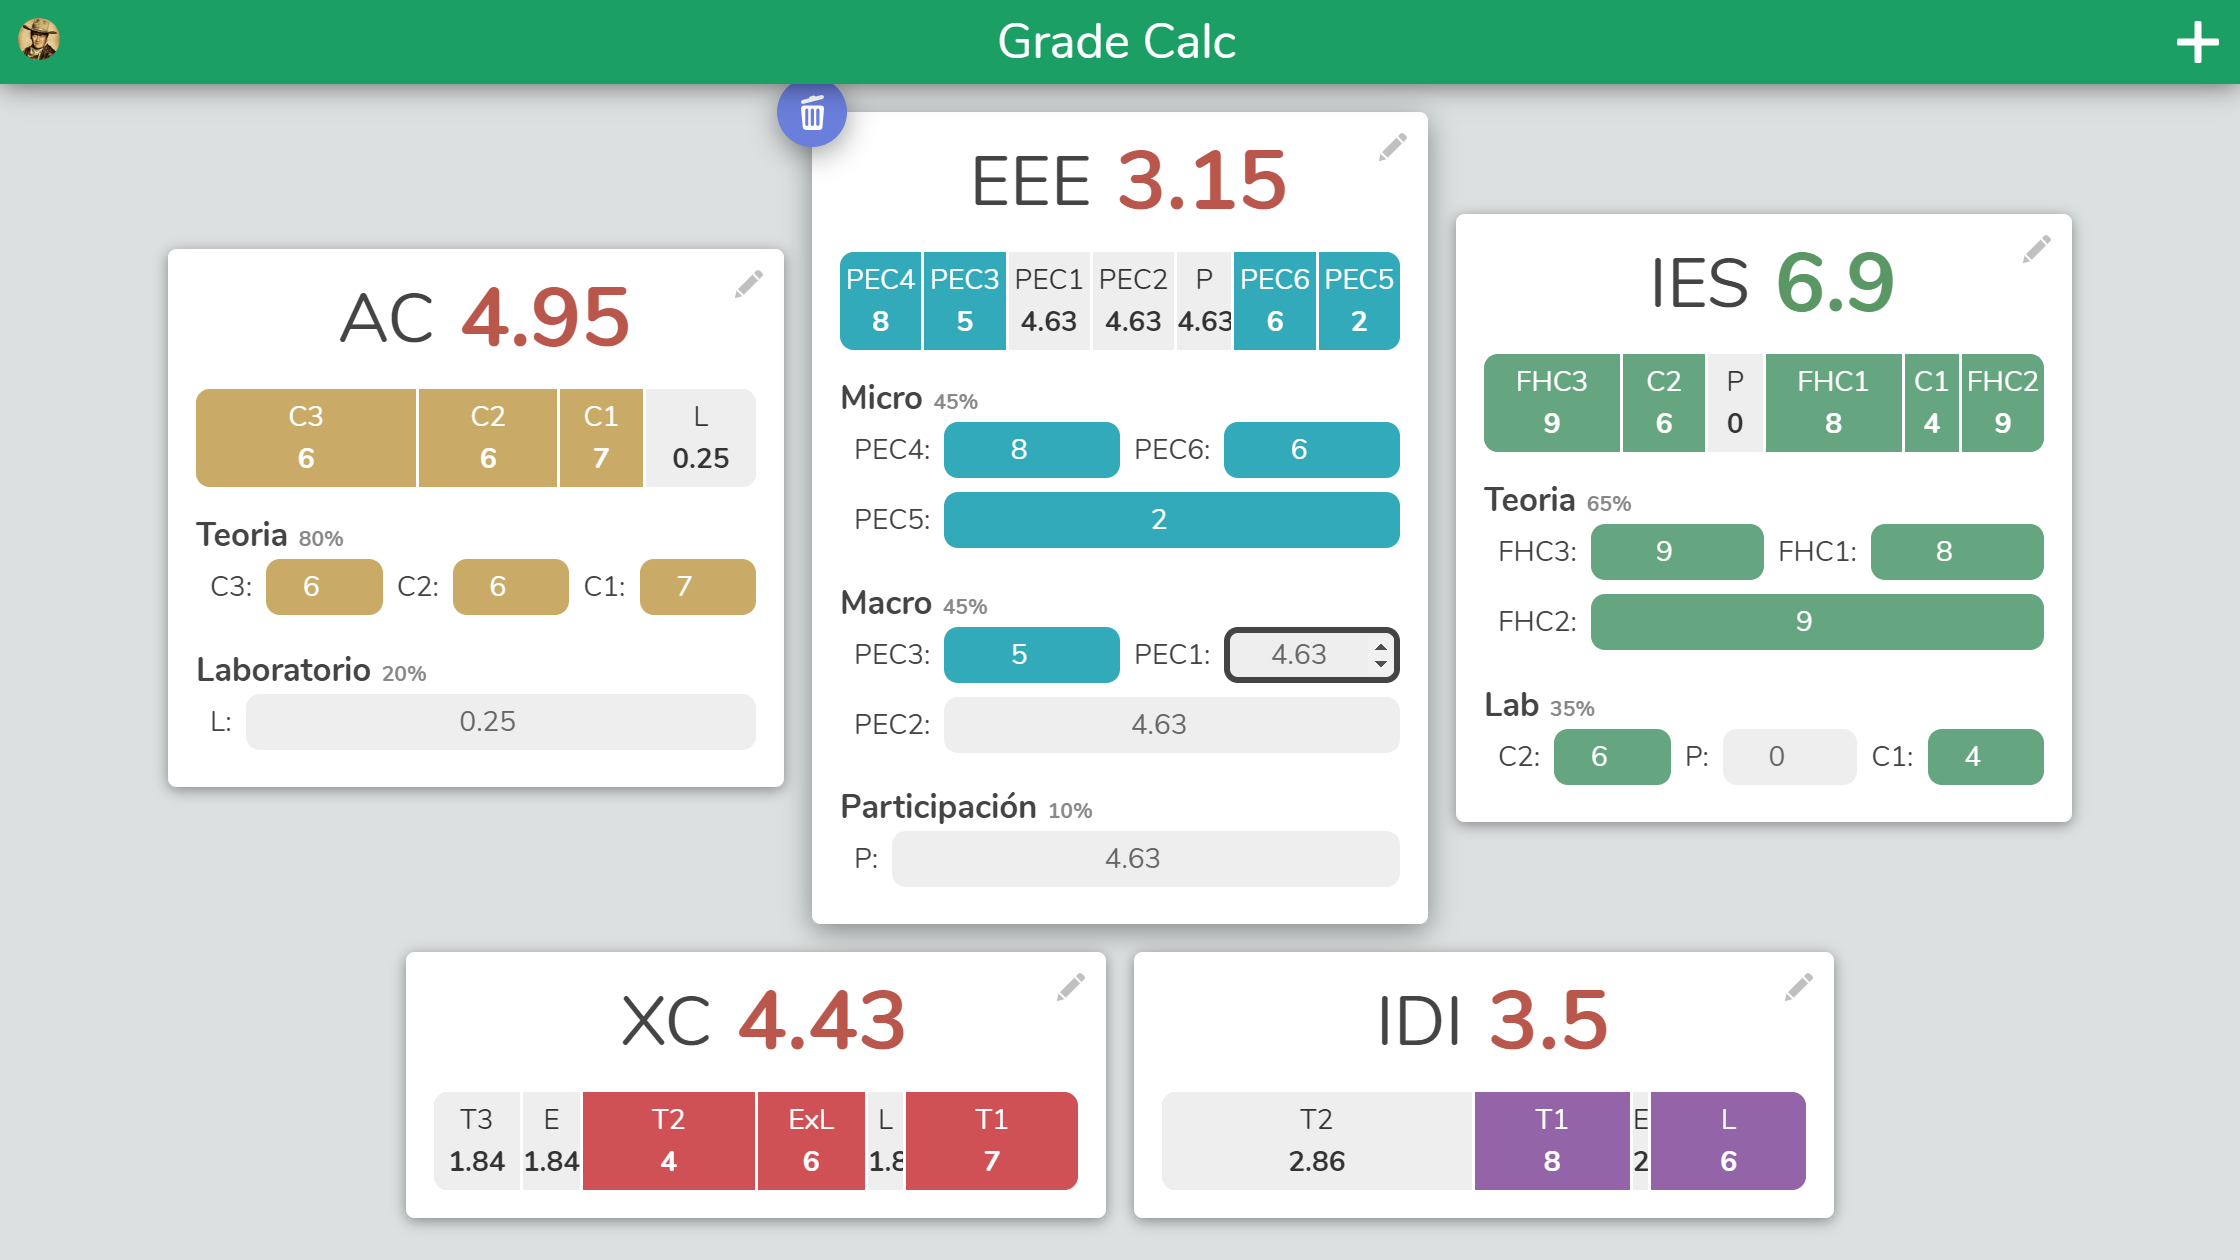
\includegraphics[width=\textwidth]{media/screenshots/screenshot-home-selected-pc.png}
        \caption{Desktop version}
    \end{subfigure}
    \hfill
    \begin{subfigure}[b]{0.243\textwidth-0.1cm}
        \centering
        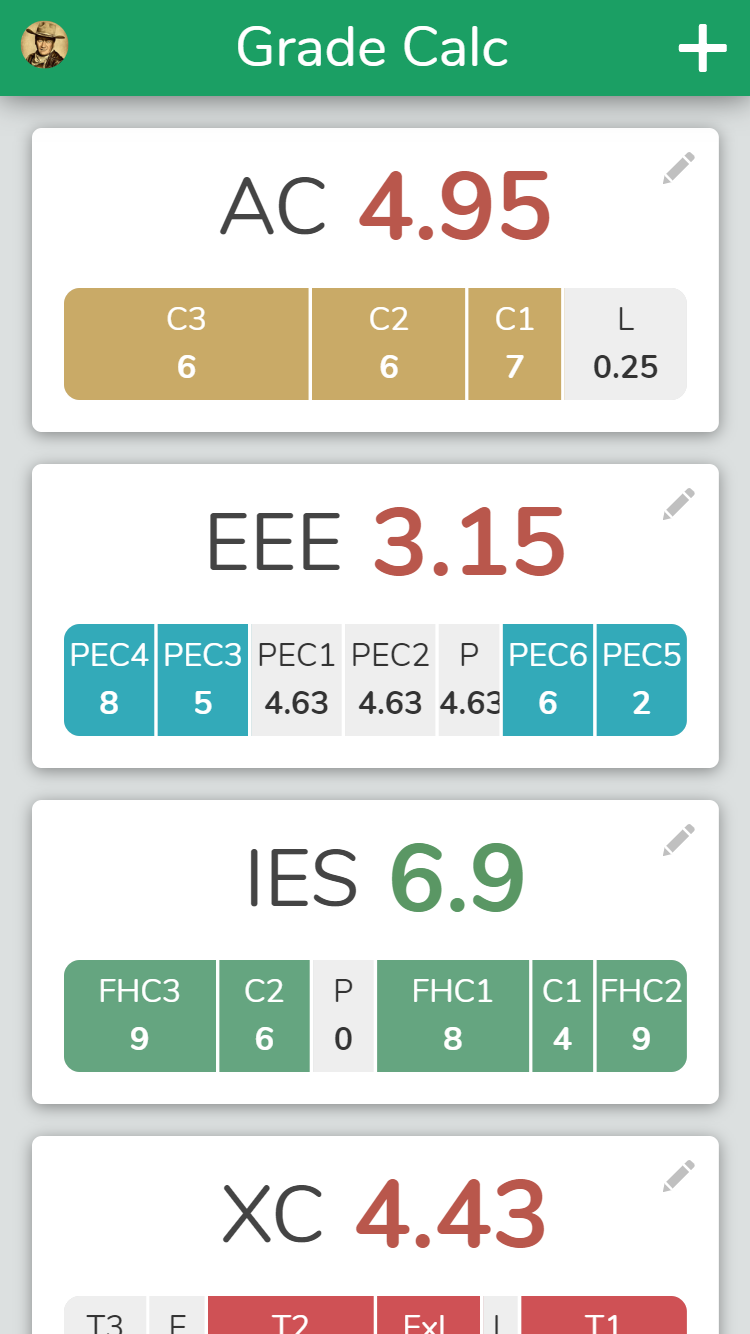
\includegraphics[width=\textwidth]{media/screenshots/screenshot-home.png}
        \caption{Mobile version}
    \end{subfigure}
    \caption{Dashboard}
    \label{fig:dashboard}
\end{figure}
\vfill

\clearpage\newpage
% \subsubsection{Welcome}

When there are no subject cards in the dashboard, the empty space is used to display a text that explains what is the app and its main features. This text is going to be the first screen of the app that a new user will see, so it aims to help them start using the app. For this reason, the last phrase of the text encourages them to press the \inlineicon{icon-plus.pdf} button. To make it more obvious, the \inlineicon{icon-plus.pdf} button starts a looping animation (rubberBand from the Animate.css\cite{animate-css} library) that draws attention to it because of its movement.

This screen serves another important purpose, it makes the app indexable by search engines like Google. In order to be searchable, the app must have some text to let Google understand what it is. So this text has to contain the keywords that we want to relate to the app.

\vfill
\begin{figure}[ht!]
    \begin{subfigure}[b]{0.757\textwidth-0.1cm}
        \centering
        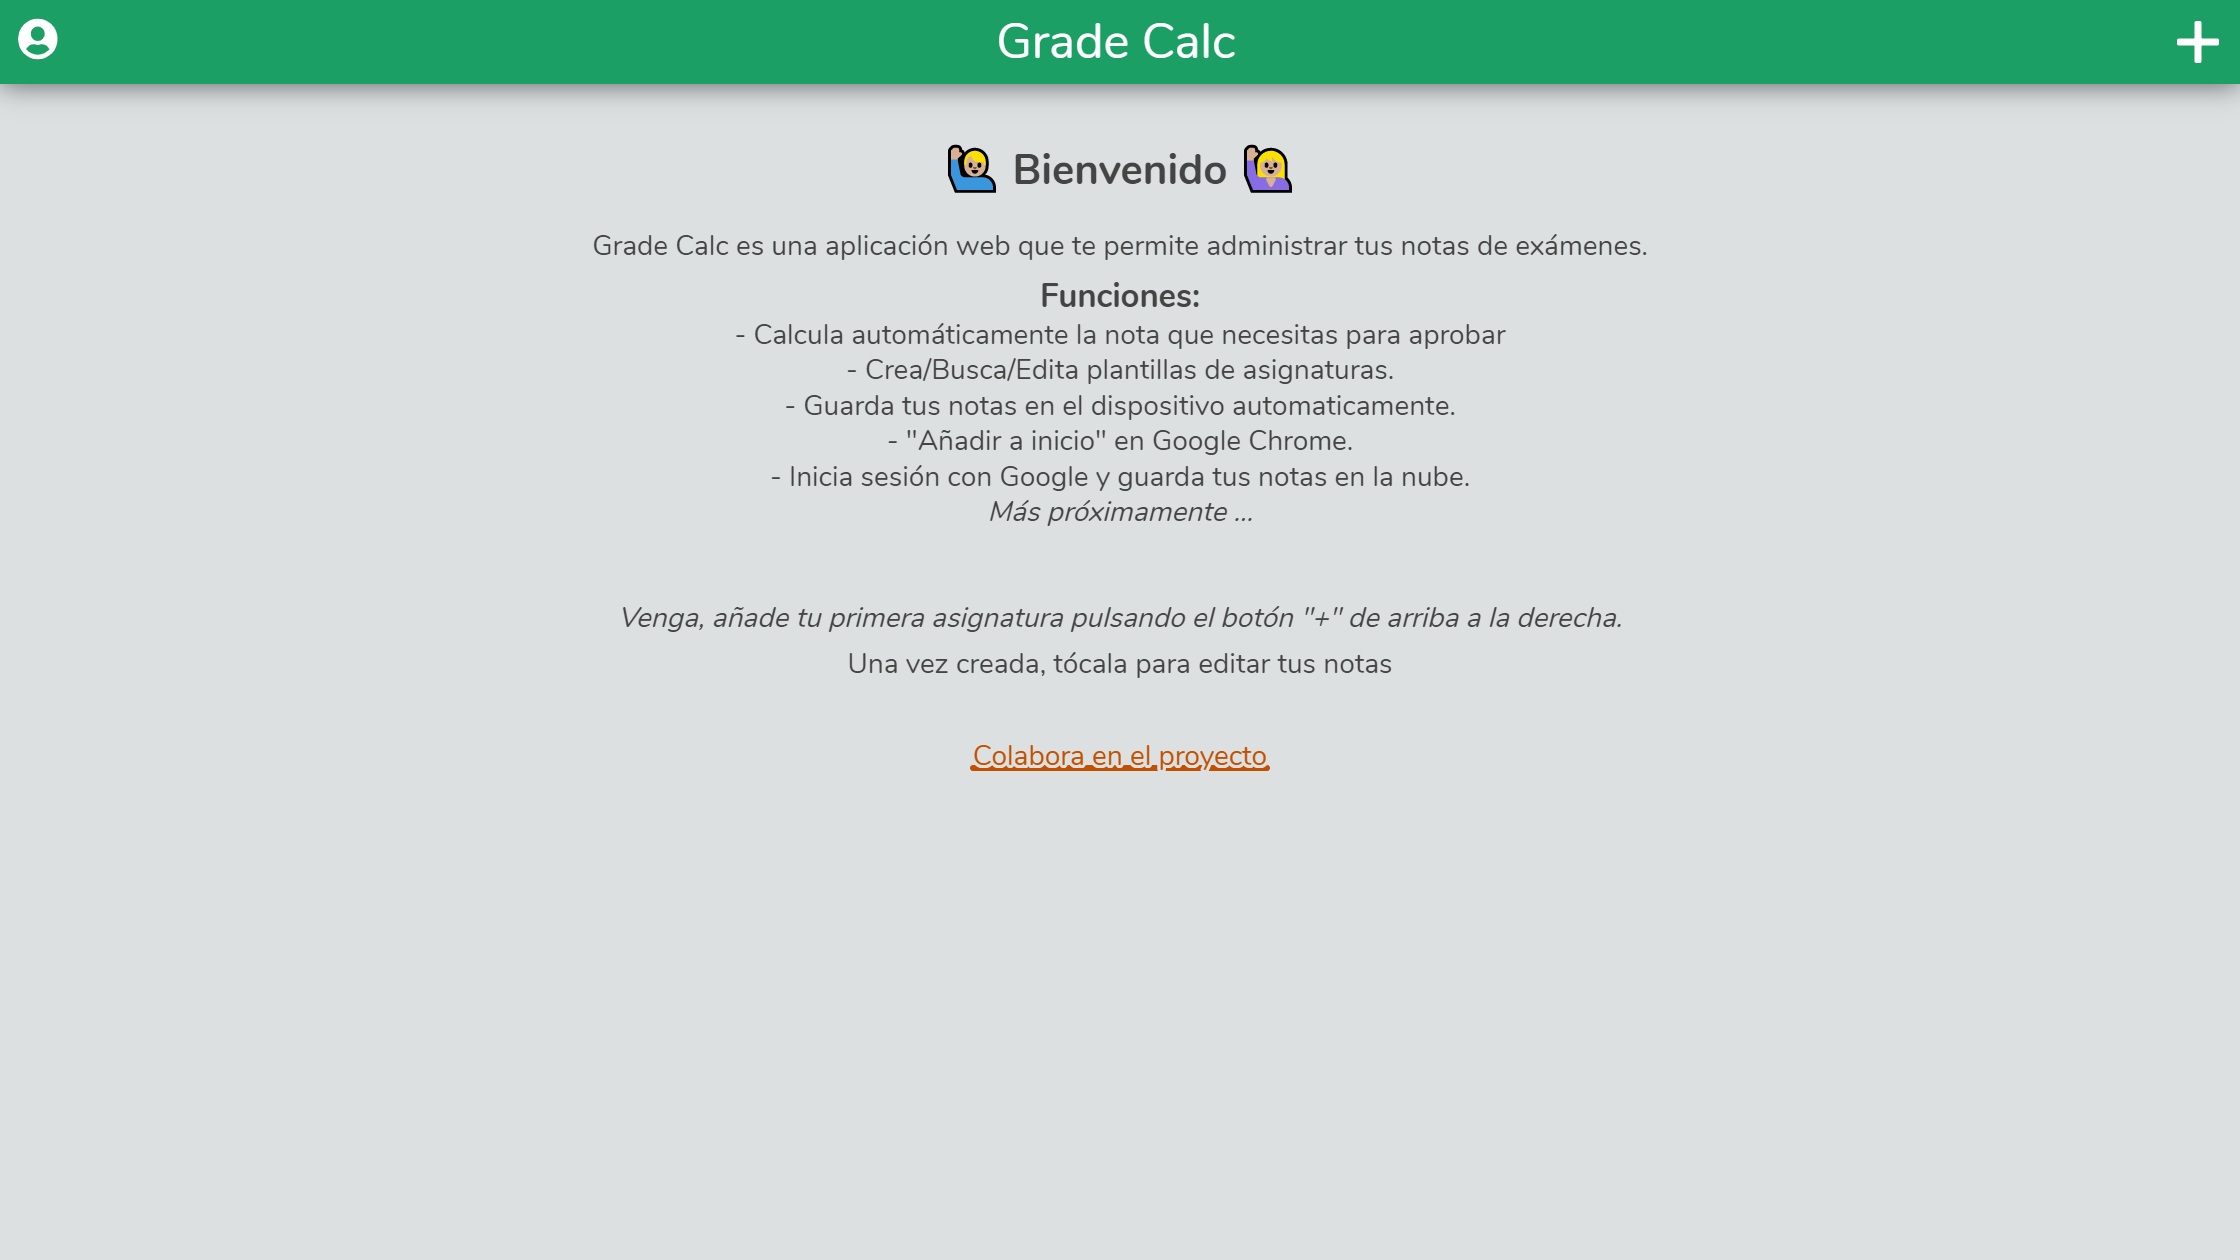
\includegraphics[width=\textwidth]{media/screenshots/screenshot-tutorial-pc.png}
        \caption{Desktop version}
    \end{subfigure}
    \hfill
    \begin{subfigure}[b]{0.243\textwidth-0.1cm}
        \centering
        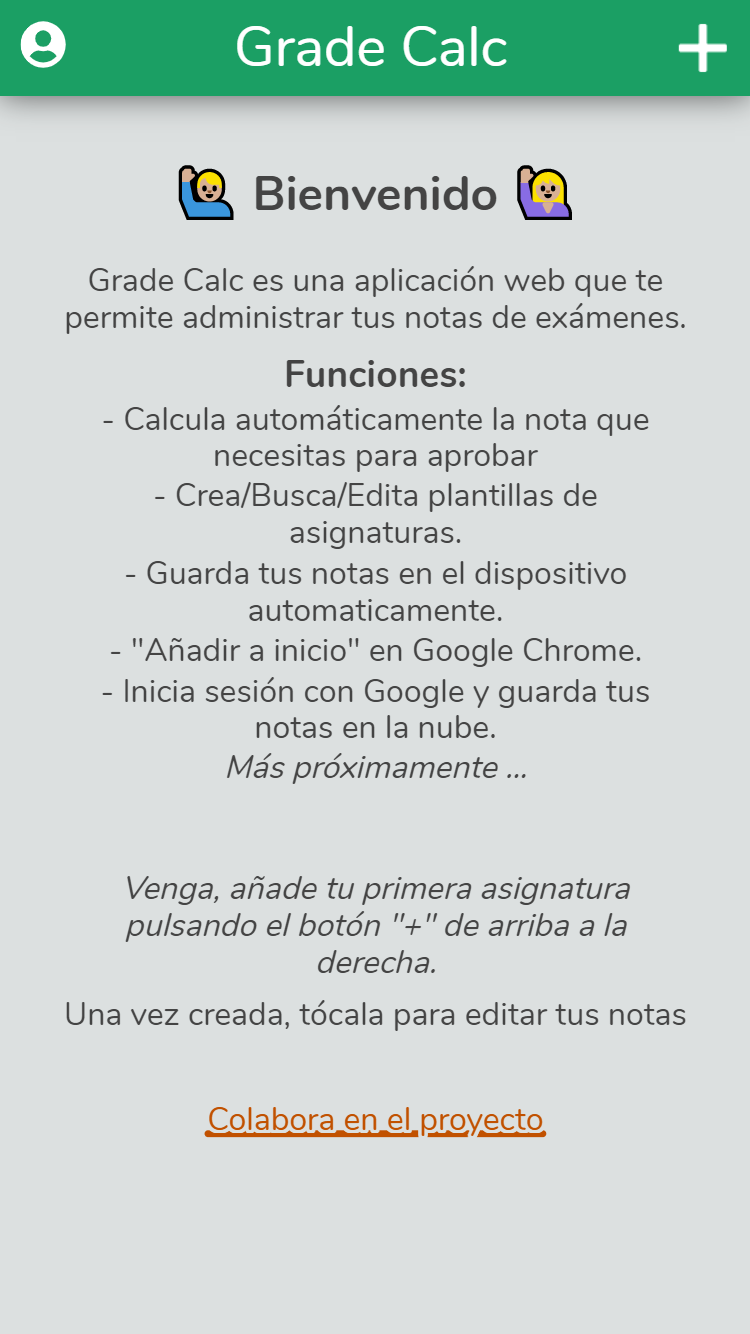
\includegraphics[width=\textwidth]{media/screenshots/screenshot-tutorial.png}
        \caption{Mobile version}
    \end{subfigure}
    \caption{Welcome}
    \label{fig:welcome}
\end{figure}
\vfill

\clearpage\newpage
\subsubsection{Subject card}
\label{sec:subject-card}

\begin{figure}[ht!]
    \begin{subfigure}[b]{0.5\textwidth-0.05cm}
        \centering
        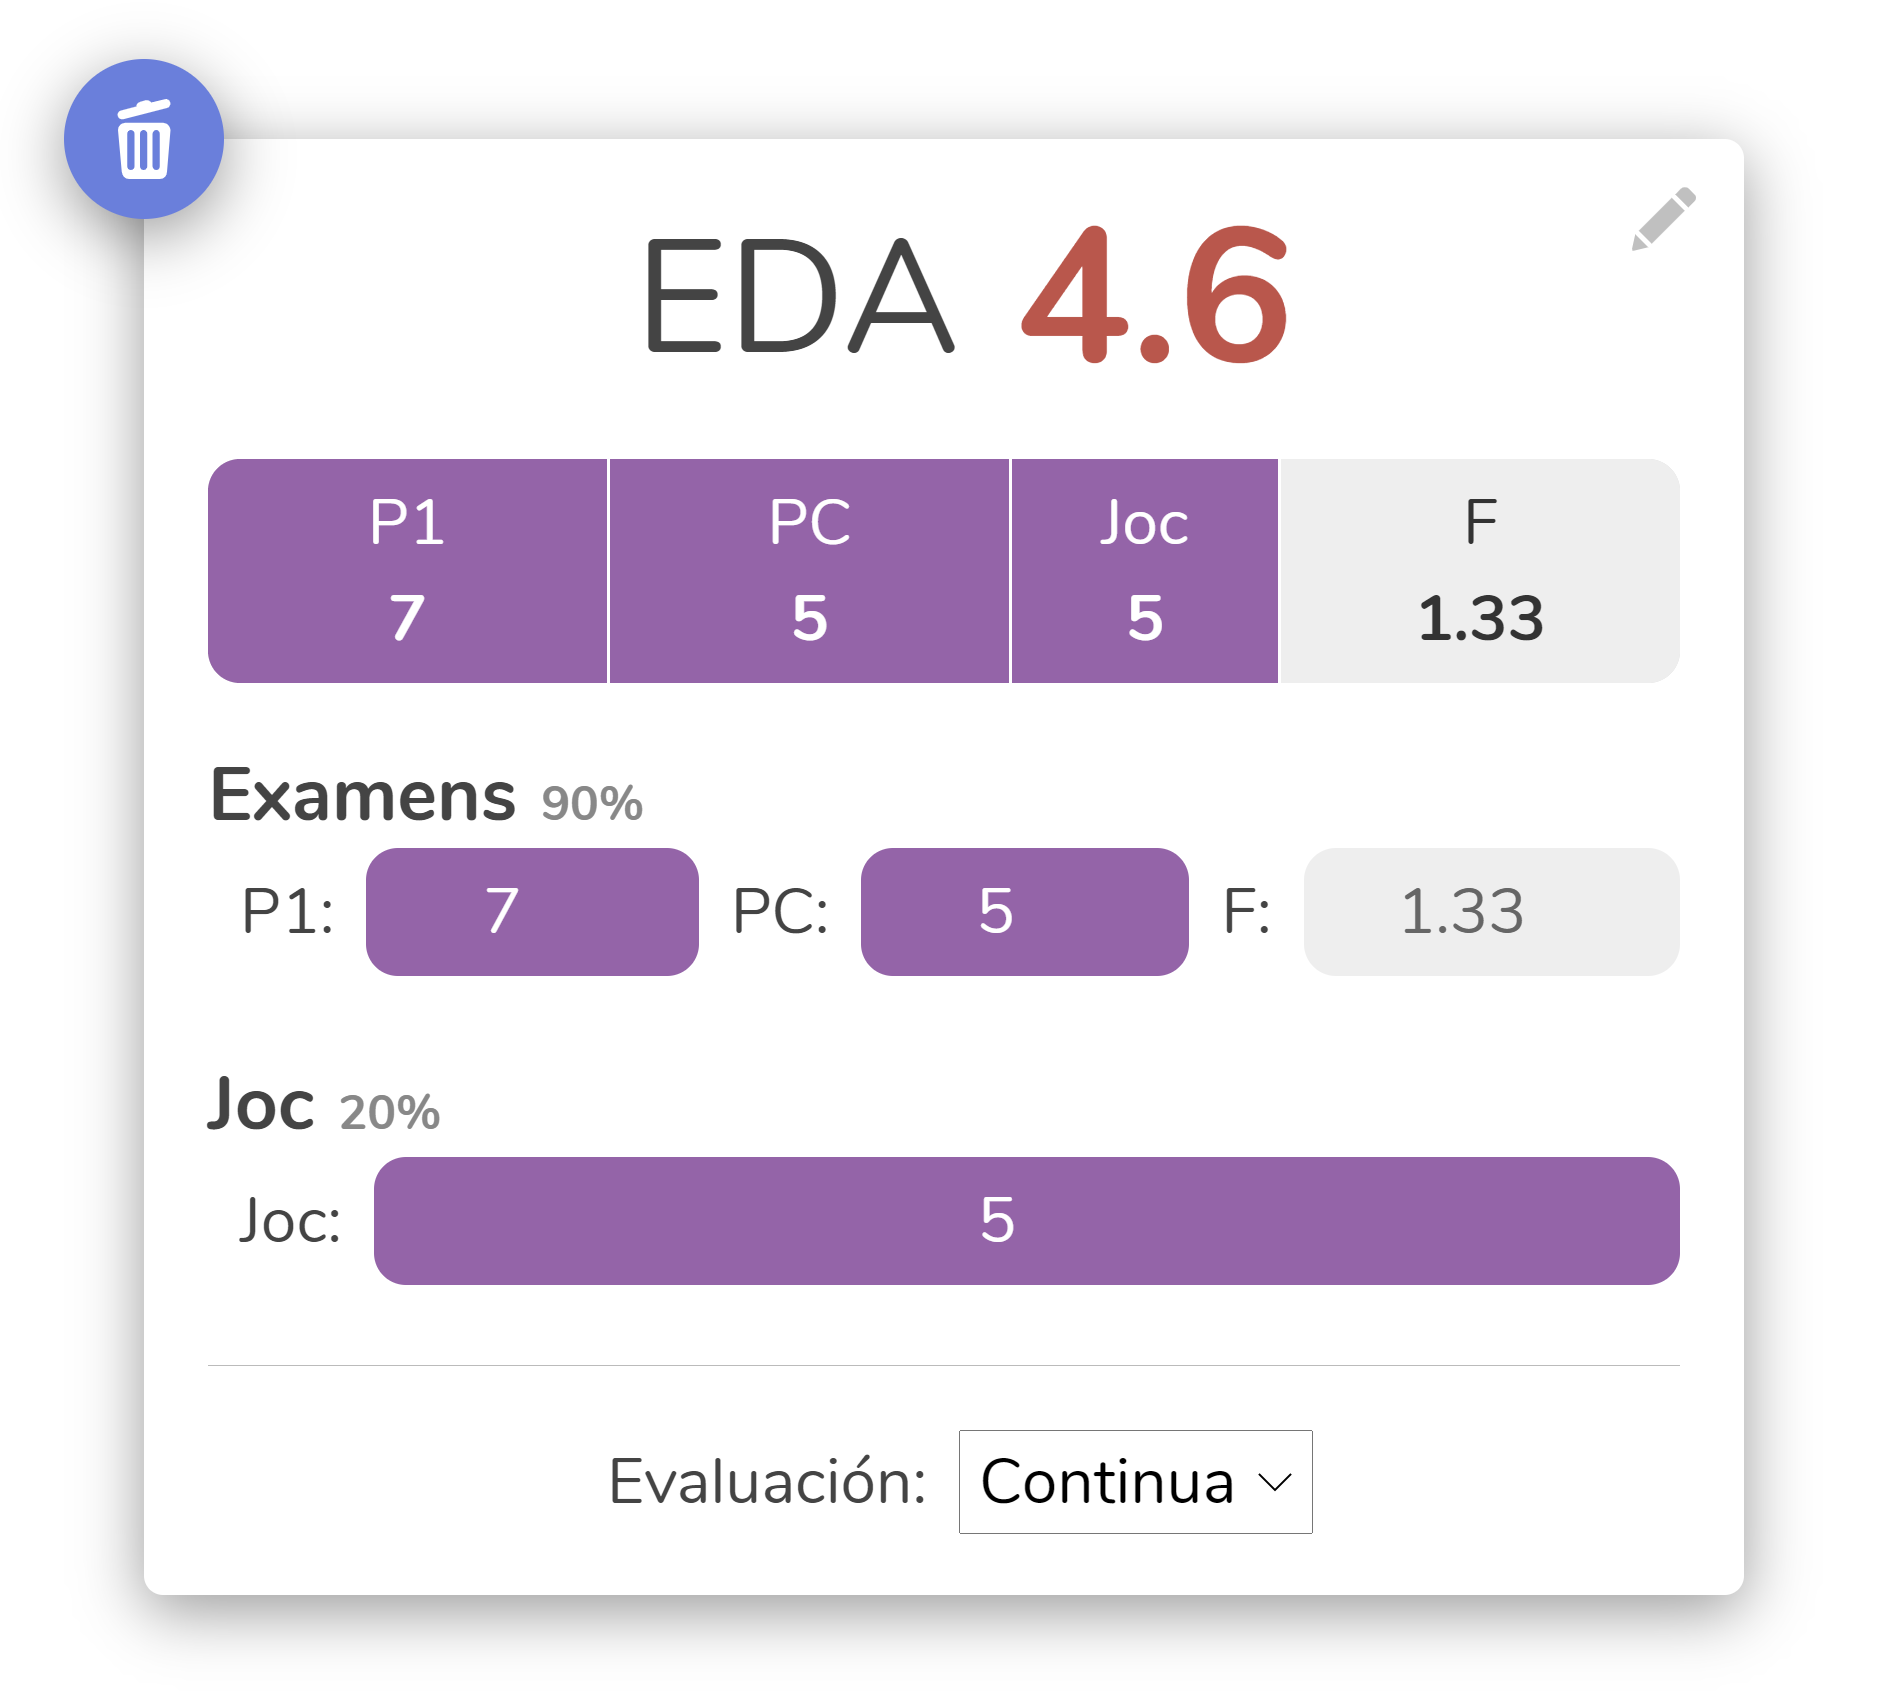
\includegraphics[width=\textwidth]{media/screenshots/screenshot-card.png}
        \caption{Clean}
    \end{subfigure}
    \hfill
    \begin{subfigure}[b]{0.5\textwidth-0.05cm}
        \centering
        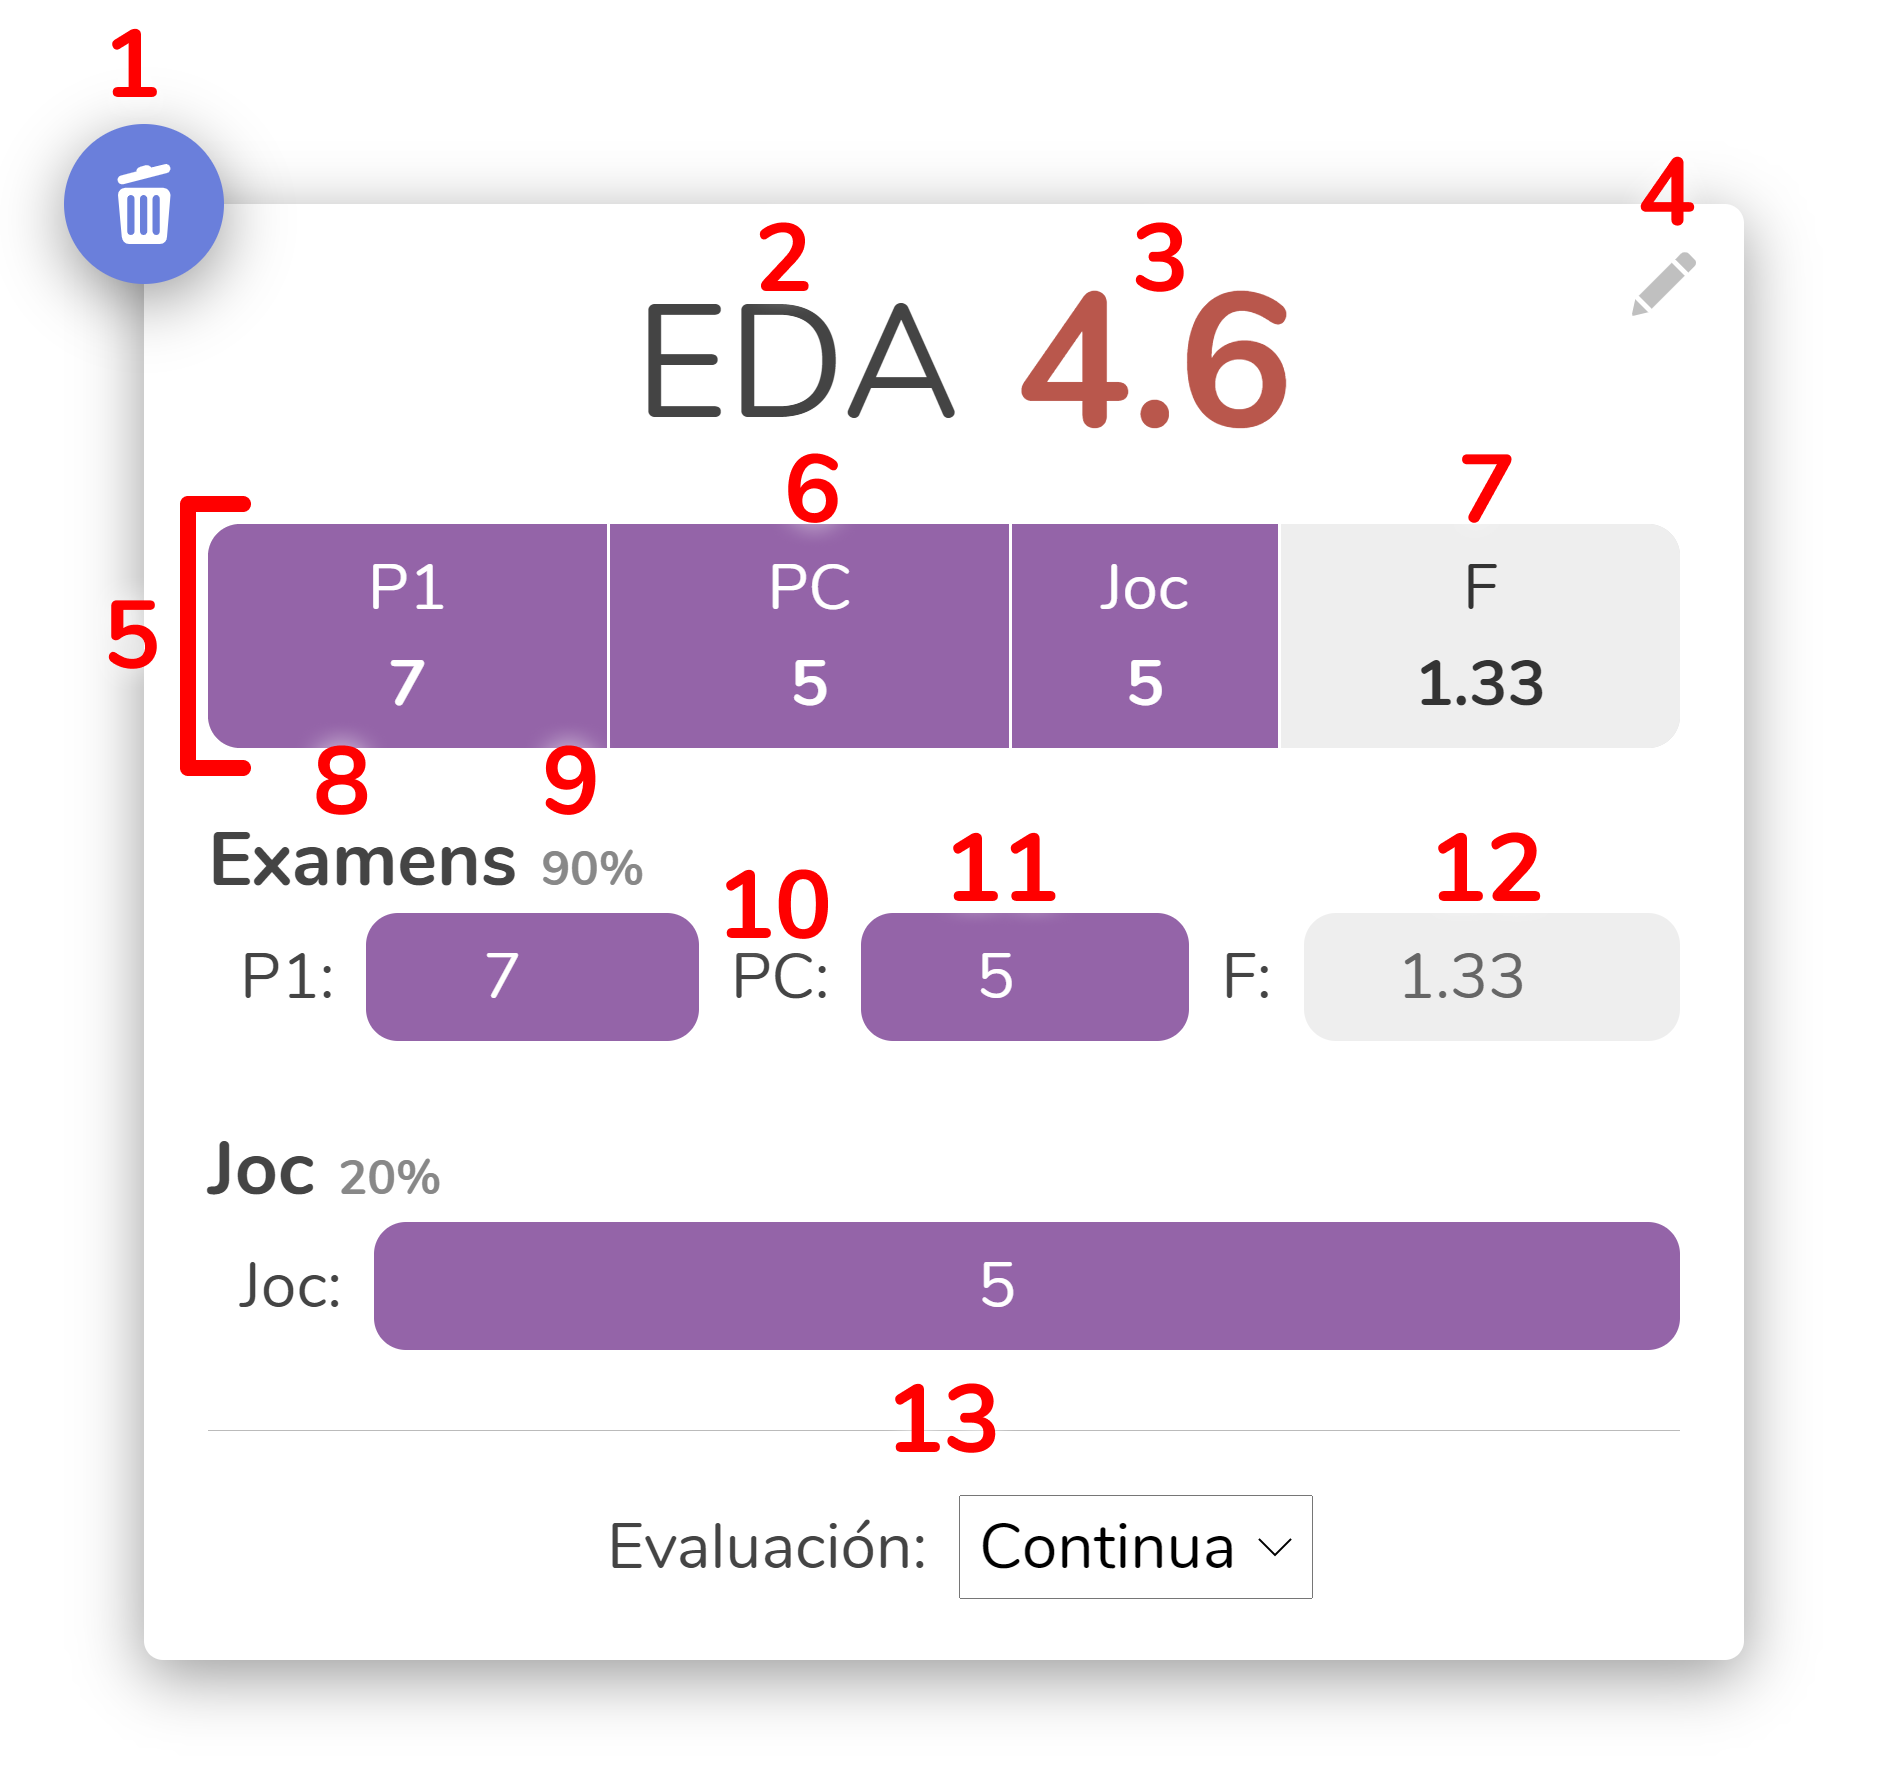
\includegraphics[width=\textwidth]{media/screenshots/screenshot-card-marked.png}
        \caption{Marked}
    \end{subfigure}
    \caption{Subject card}
    \label{fig:card}
\end{figure}

This is a subject card (Fig. \ref{fig:card}). It's the component that users interact with most of their time in the app, so it is very optimized in terms of usability. 

It is important to define what is \textit{necessary grade}. The \textbf{necessary grade} is the necessary grade to receive in all the remaining exams to get a 5 in the final grade. % In this case, it's 1.33 because if the student receives a 1.33 in the \textit{F} exam (the only remaining exam) the final grade will be a 5.

When a card is clicked, it's expanded or collapsed depending on its previous state.

The card's information is updated in real-time as the student changes the grades. This means that the final and necessary grades are calculated every time a value changes automatically. This feature enables users to quickly test several combinations of grades to find the one that will make them pass the subject.

% \begin{multicols}{2}
\begin{enumerate}[itemsep=0mm]
    \item \textbf{Delete button}: When hovered\footnote{Hover means placing the mouse cursor on top of an element without clicking it} the button shakes indicating (like it is afraid of being clicked) that indicates that the button is dangerous. \\
    When clicked the card disappears and another animation occurs, the cards move smoothly to their new positions. Without the animation, it's very disorienting for the user, it's unclear where each card went, especially when they change row. This is not a trivial animation and I had to code it\cite{flex-animation}.
    \item \textbf{Short name}: The short name of the subject, usually it's initial letters.
    \item \textbf{Current grade}: The current final grade calculated with the filled exam inputs and assuming a 0 in the remaining exams. It's rounded to two decimal places. If it's lower than 5, it's red and if its greater or equal than 5, green. This indicates whether the subject is passed or failed. \\
    When this value changes from red to green the confetti animation is triggered. Confetti is shooted on the card celebrating that the student passed the subject.
    \item \textbf{Edit button}: When clicked, the edit screen (Fig. \ref{fig:edit}) of the subject is opened. There the exam weights can be modified, among other things.
    \item \textbf{Evaluation representation}: It's a bar that contains all exams in the evaluation where the width of every exam is proportional to its weight. This is a simple and comprehensible graphical representation of all the exams' weighs. \\
    When a section is clicked the respective exam input is focused and the student can start typing the grade in the input field. And when it's hovered a hint below the cursor shows up, indicating the exact weight of the exam. 
    \item \textbf{Exam representation (done)}: The background color is the subject's color and the number is the received grade.
    \item \textbf{Exam representation (undone)}: The background color is light gray and the number is the necessary grade. 
    \item \textbf{Exam type}: It's a section that contains the exams with that type of selected evaluation. In the example, there are 3 exams with the type \textit{Examens}. % The exams are displayed in rows of up to 3 exams.
    \item \textbf{Exam type weight}: This number represents the sum of weights of the exams inside the section. In this case, 90\% is the sum of the weights of the exams \textit{P1}, \textit{PC} and \textit{F}. This is helpful when there are many exams inside one category that are weighted very little because the category takes more space it seems more weighted but it is not always the case. In Figure \ref{fig:dashboard} you can see its use in the purple subject \textit{F}.
    \item \textbf{Exam name}: This is the label of the input to the right, it contains the name of the exam. When clicked the input is focused.
    \item \textbf{Grade input (done)}: he background color is the subject's color and the value is the received grade.
    \item \textbf{Grade input (undone)}: The background color is light gray and the value is a placeholder with is the necessary grade. When the user types something, the number is overwritten without the need of deleting it.
    \item \textbf{Selected evaluation}: This is a dropdown with all possible evaluations. If there's only one evaluation it's hidden.
\end{enumerate}
% \end{multicols}

\vfill
\begin{figure}[ht!]
    \begin{subfigure}[b]{0.757\textwidth-0.1cm}
        \centering
        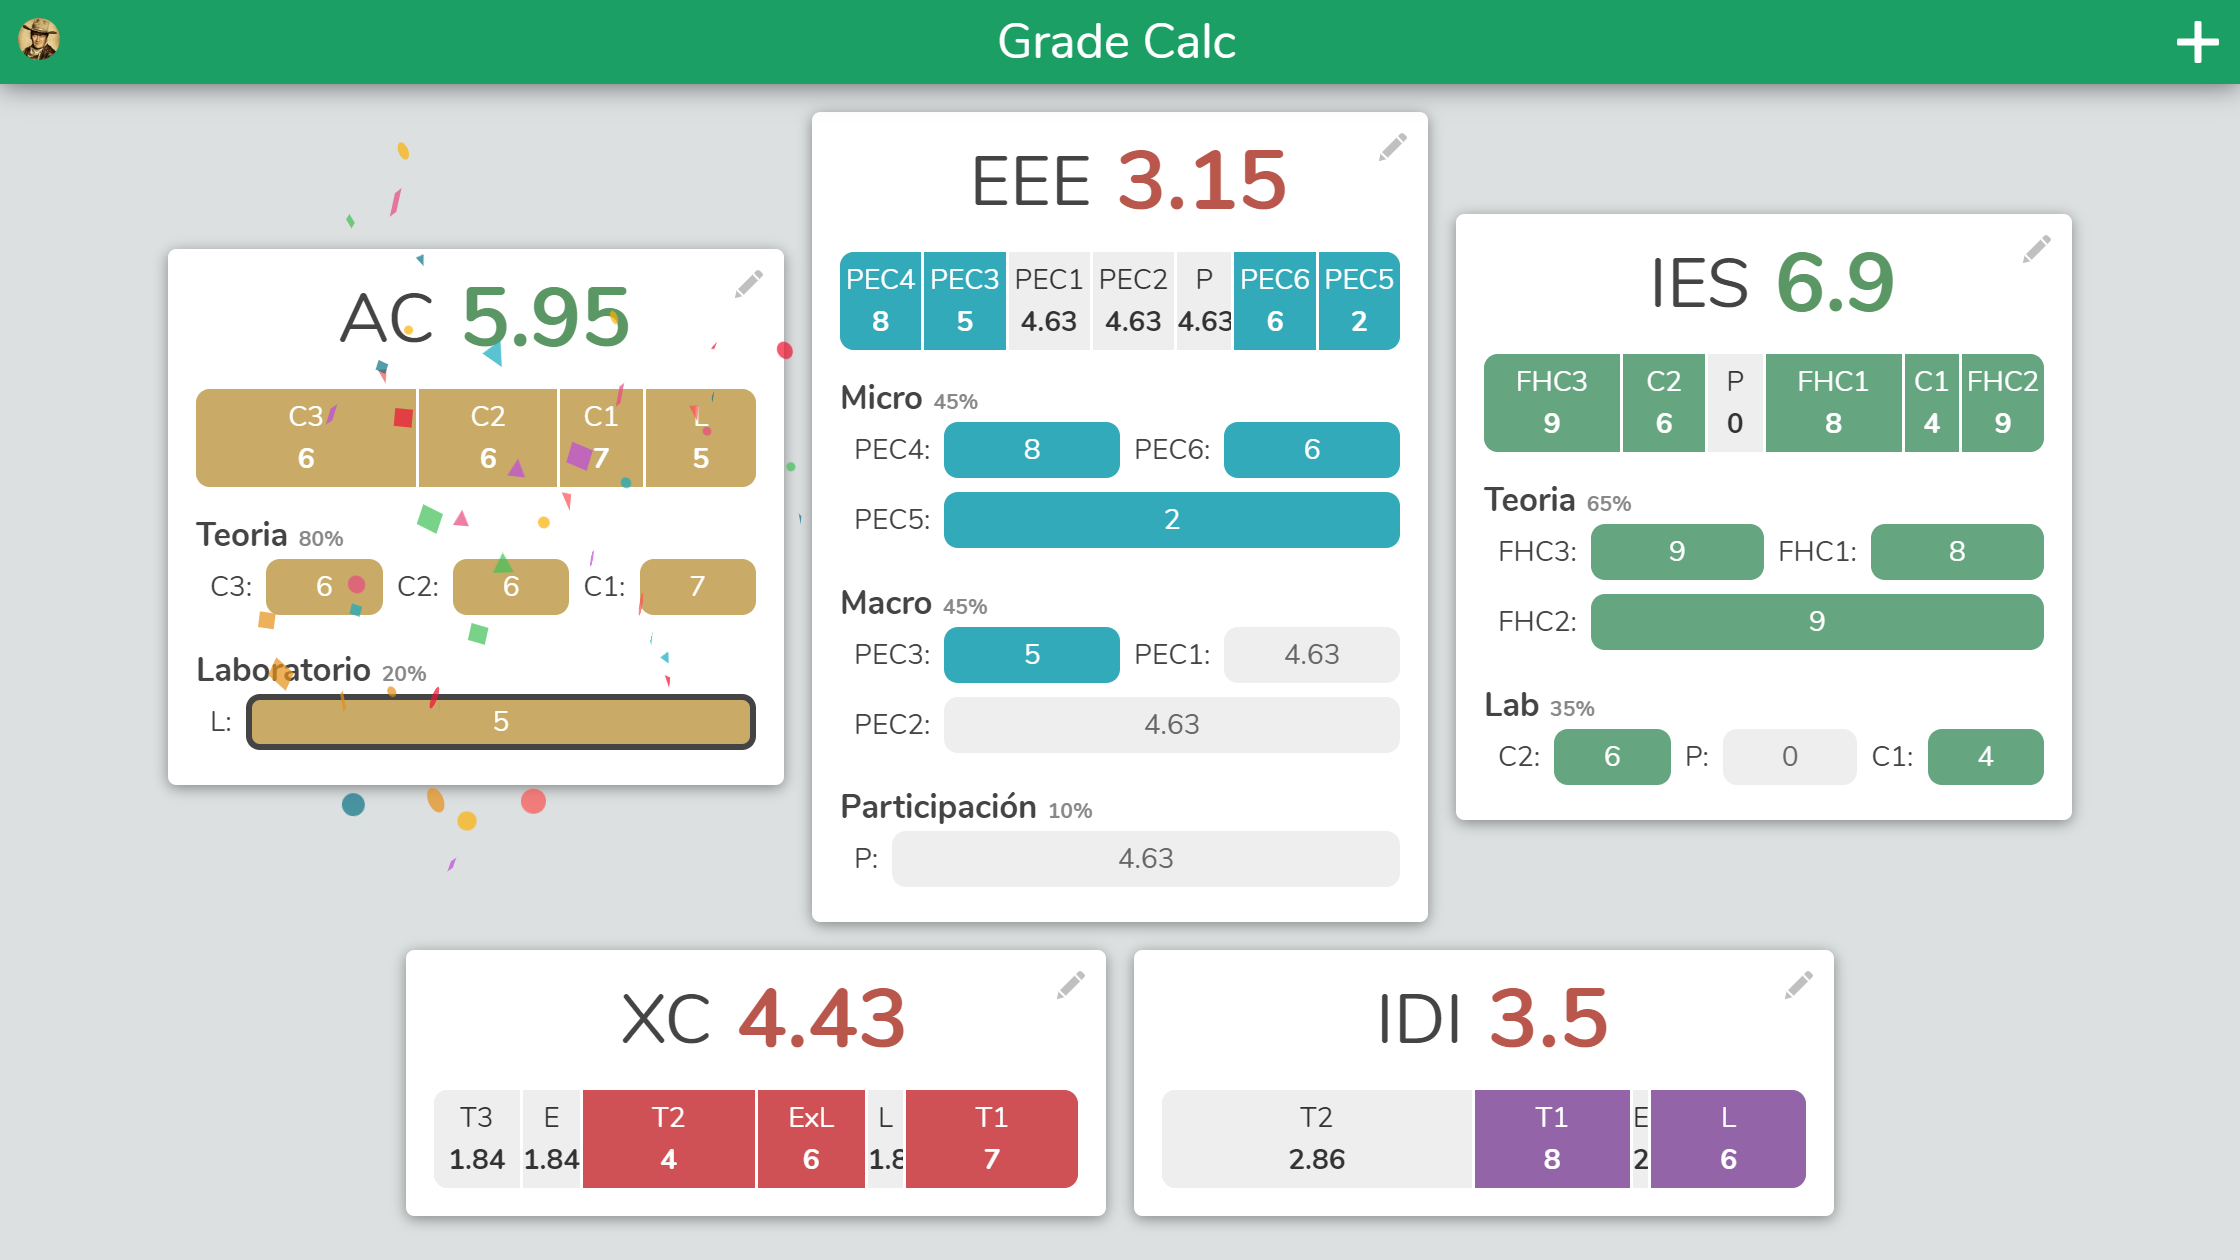
\includegraphics[width=\textwidth]{media/screenshots/screenshot-confetti-pc.png}
        \caption{Desktop version}
    \end{subfigure}
    \hfill
    \begin{subfigure}[b]{0.243\textwidth-0.1cm}
        \centering
        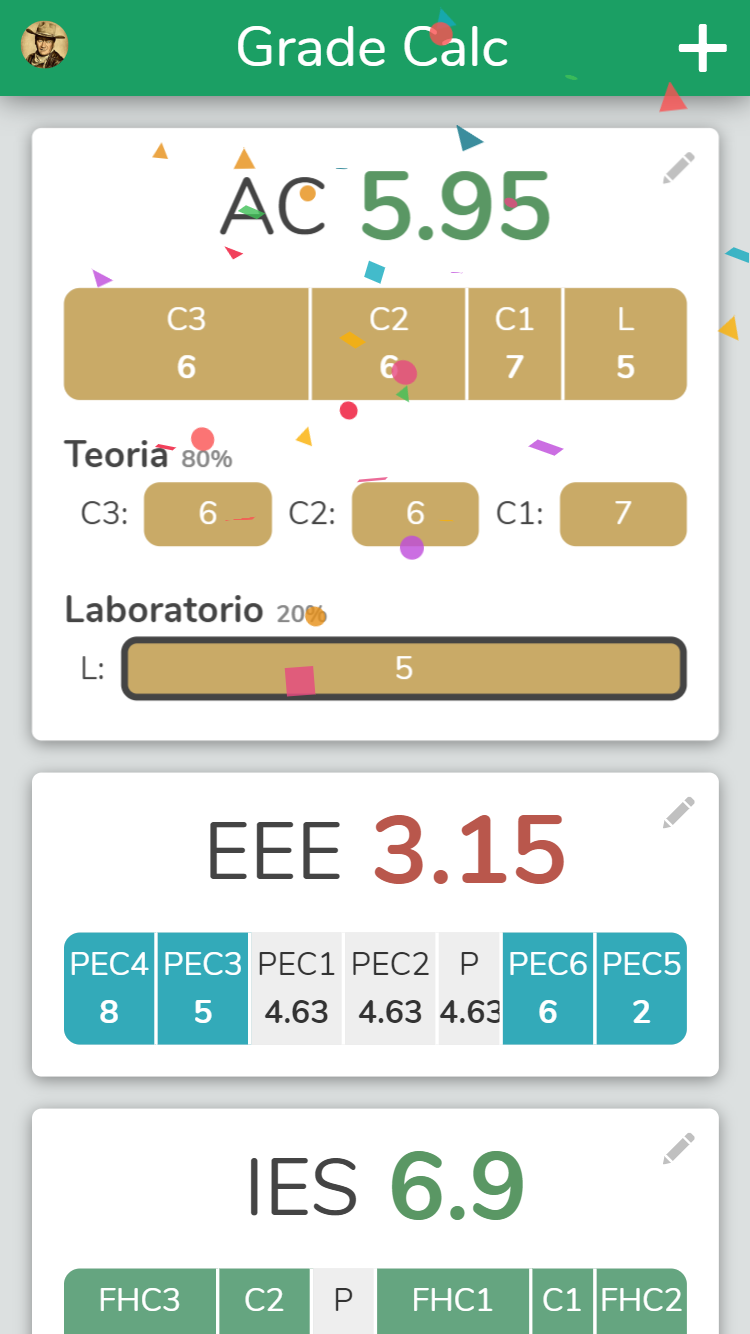
\includegraphics[width=\textwidth]{media/screenshots/screenshot-confetti.png}
        \caption{Mobile version}
    \end{subfigure}
    \caption{Confetti}
    \label{fig:confetti}
\end{figure}
\vfill

\clearpage\newpage
\subsubsection{Search subjects}

When the user clicks the \inlineicon{icon-plus.pdf} button from the dashboard (Fig. \ref{fig:dashboard}) this screen appears. In the desktop, it's a popup and in the mobile, it uses the entire screen. Here the user can:
\begin{enumerate}[itemsep=0mm]
    \item Go back by clicking the \inlineicon{icon-back.pdf} button, clicking the popup background, or clicking the back button from the browser or mobile.
    \item Open the create screen (Fig.  \ref{fig:create}) by clicking the \inlineicon{button-create-gray.png} button.
    \item Show search results by typing in the search input.
    \item Add the selected subjects to the dashboard and go to the dashboard by clicking the \inlineicon{button-add.png} button. If there isn't any subject selected it just goes to the dashboard
\end{enumerate}

The \inlineicon{button-create-gray.png} button is in gray to not draw much attention. The app doesn't have a system to manage duplicate information, so we try to guide users into reusing subjects instead of creating new ones. The search field is automatically focused, and in mobile, the keyboard pops up automatically, this makes user start typing instead of clicking the \inlineicon{button-create-gray.png} button.

\vfill
\begin{figure}[ht!]
    \begin{subfigure}[b]{0.757\textwidth-0.1cm}
        \centering
        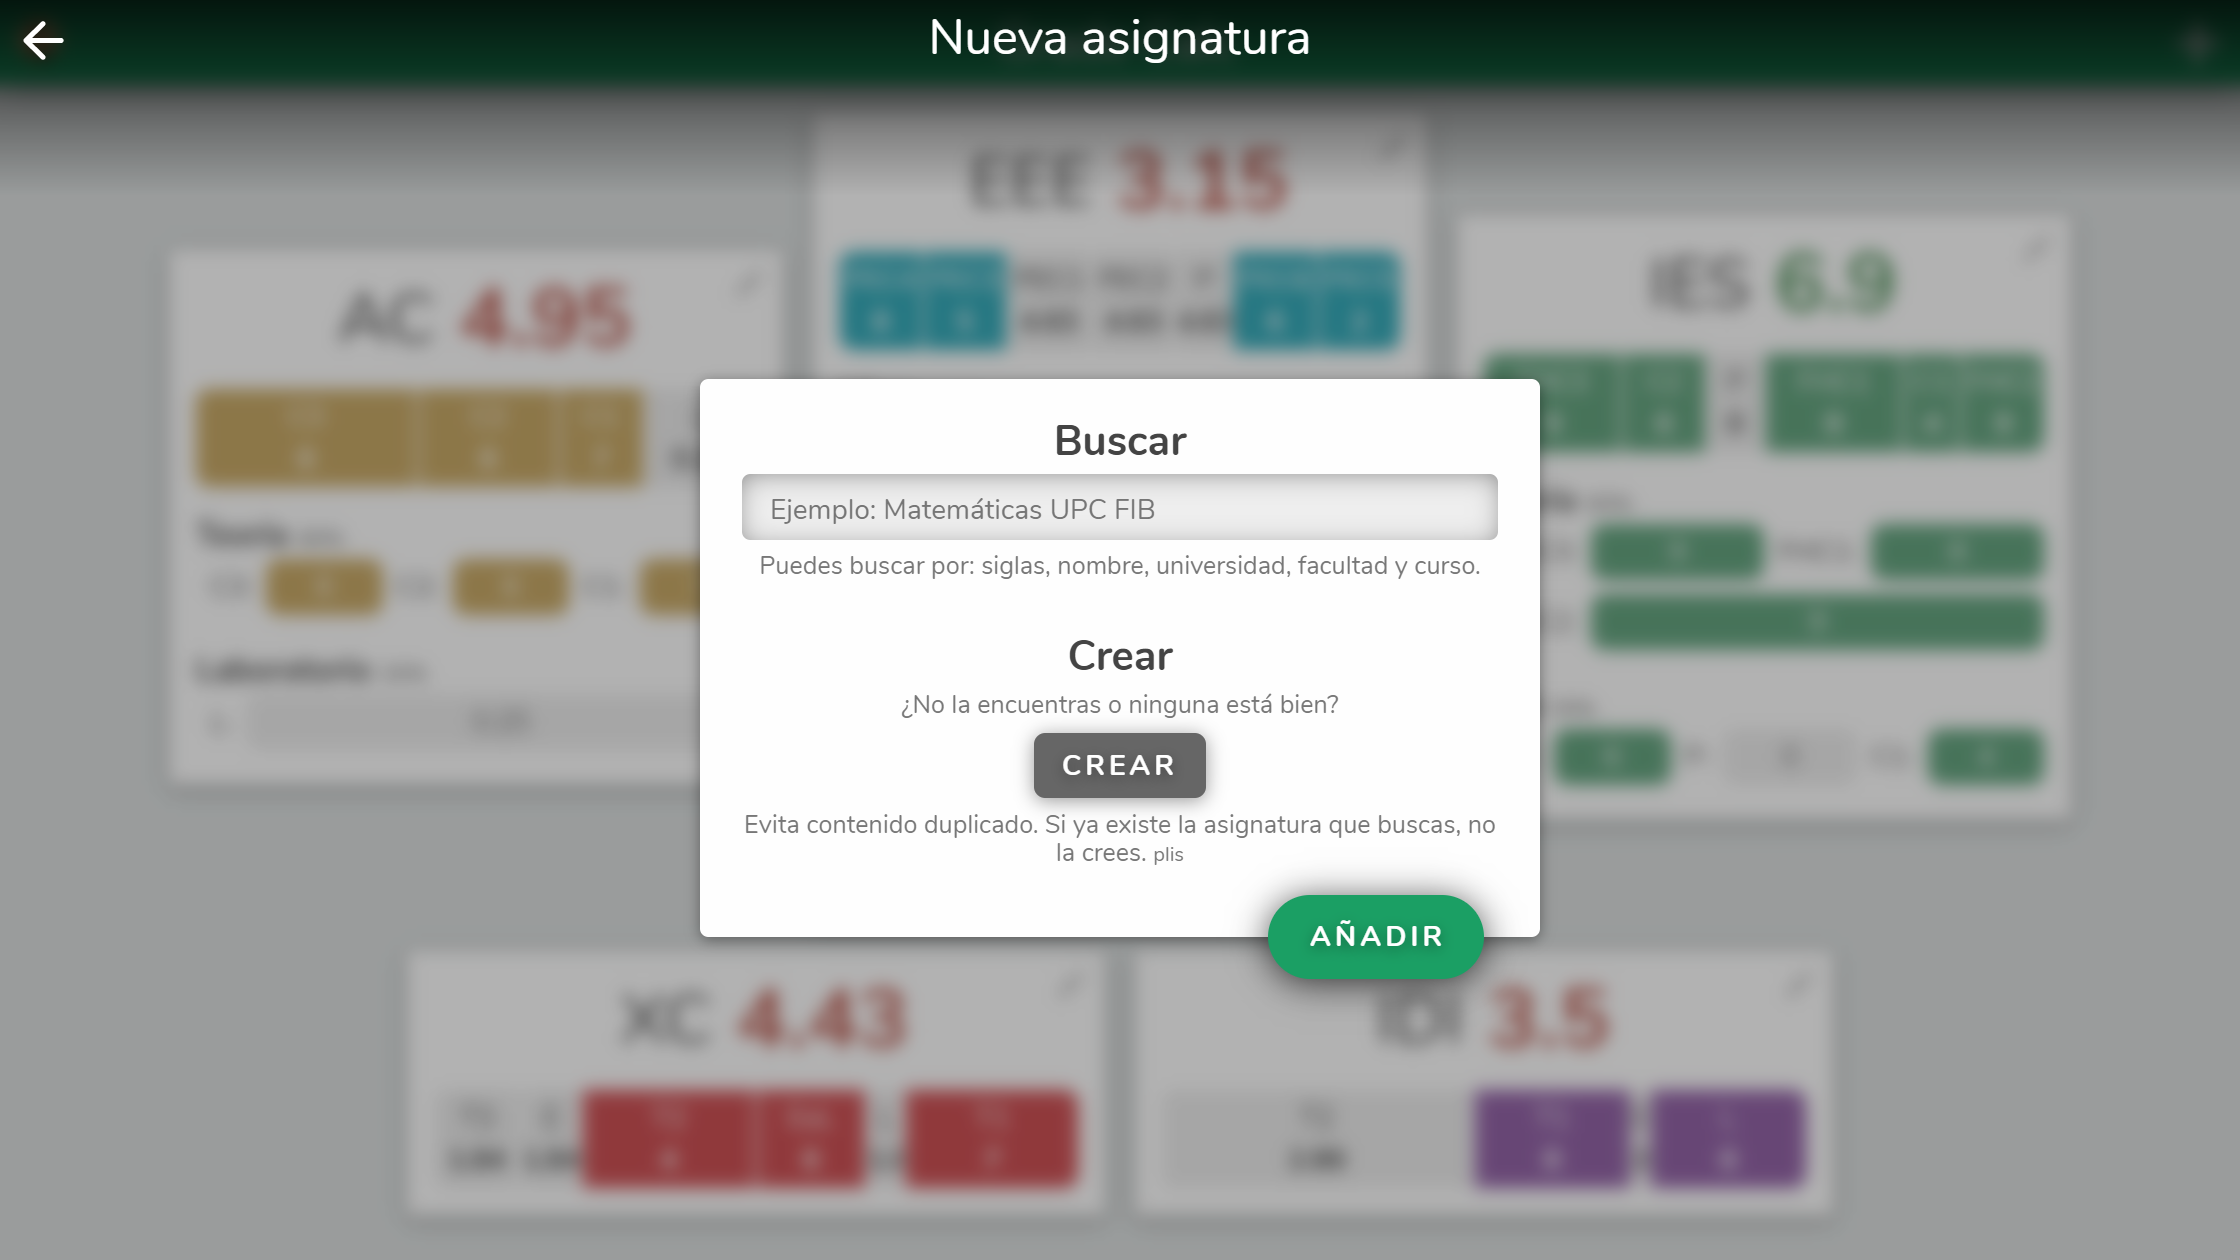
\includegraphics[width=\textwidth]{media/screenshots/screenshot-search-empty-pc.png}
        \caption{Desktop version}
    \end{subfigure}
    \hfill
    \begin{subfigure}[b]{0.243\textwidth-0.1cm}
        \centering
        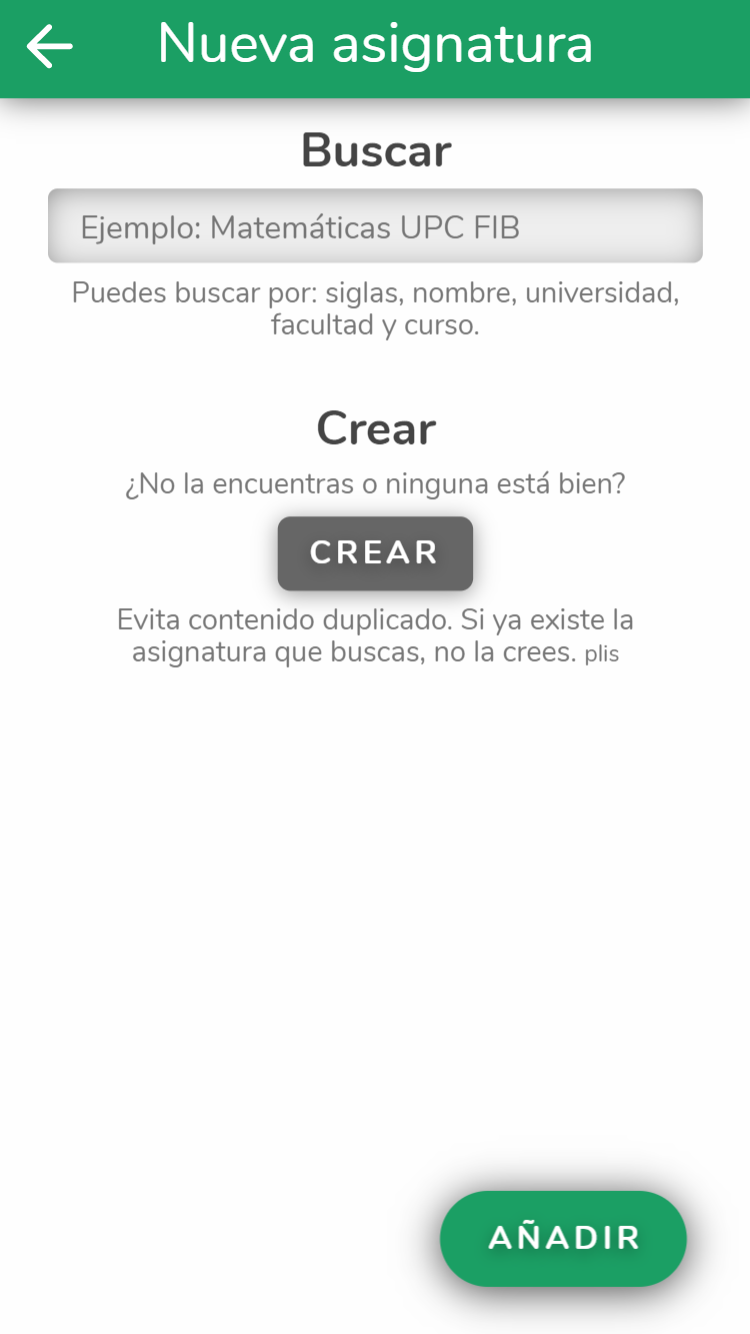
\includegraphics[frame,width=\textwidth]{media/screenshots/screenshot-search-empty.png}
        \caption{Mobile version}
    \end{subfigure}
    \caption{Search subjects empty input}
    \label{fig:search-empty}
\end{figure}
\vfill

\clearpage\newpage
Notice that when the search input is empty (Fig. \ref{fig:search-empty}) a there is a placeholder displaying an example, this is a way to teach users what can they search without explaining it. % Once he has typed something there are two options, there are matching results or there are not.

The instant search engine performs a search each time a key is pressed, showing the 20 most relevant results. The fields relevance depends on what attribute the match occurs, being in this order \textit{shortName} > \textit{longName} > \textit{course} > \textit{faculty} > \textit{university}. The search engine is typo-tolerant in \textit{English}, \textit{Spanish} and \textit{Catalan}, notice the typo in the (Fig. \ref{fig:search-filled}). The results have the matching parts highlighted to help the user understand why they are there. It also keeps a record of the queries, so I can search what is the subject that more people are looking for and also the queries that don't provide any result.

Having instant search makes the app feel really fast and responsive. And with its configurations, it ensures that the users find what they are looking for on the first query. 

Once the search results are on the screen the student can click the empty checkboxes  \inlineicon{button-search-empty.png} and check them \inlineicon{button-search-green.png} to add those subjects to the dashboard when the \inlineicon{button-add.png} is pressed. If the checkbox is disabled \inlineicon{button-search-gray.png} it means that the subject is already added. When the \inlineicon{icon-edit.pdf} button is clicked the edit subject screen is opened (Fig. \ref{fig:edit}) this way the user can check that the evaluation is correct. 

\vfill
\begin{figure}[ht!]
    \begin{subfigure}[b]{0.757\textwidth-0.1cm}
        \centering
        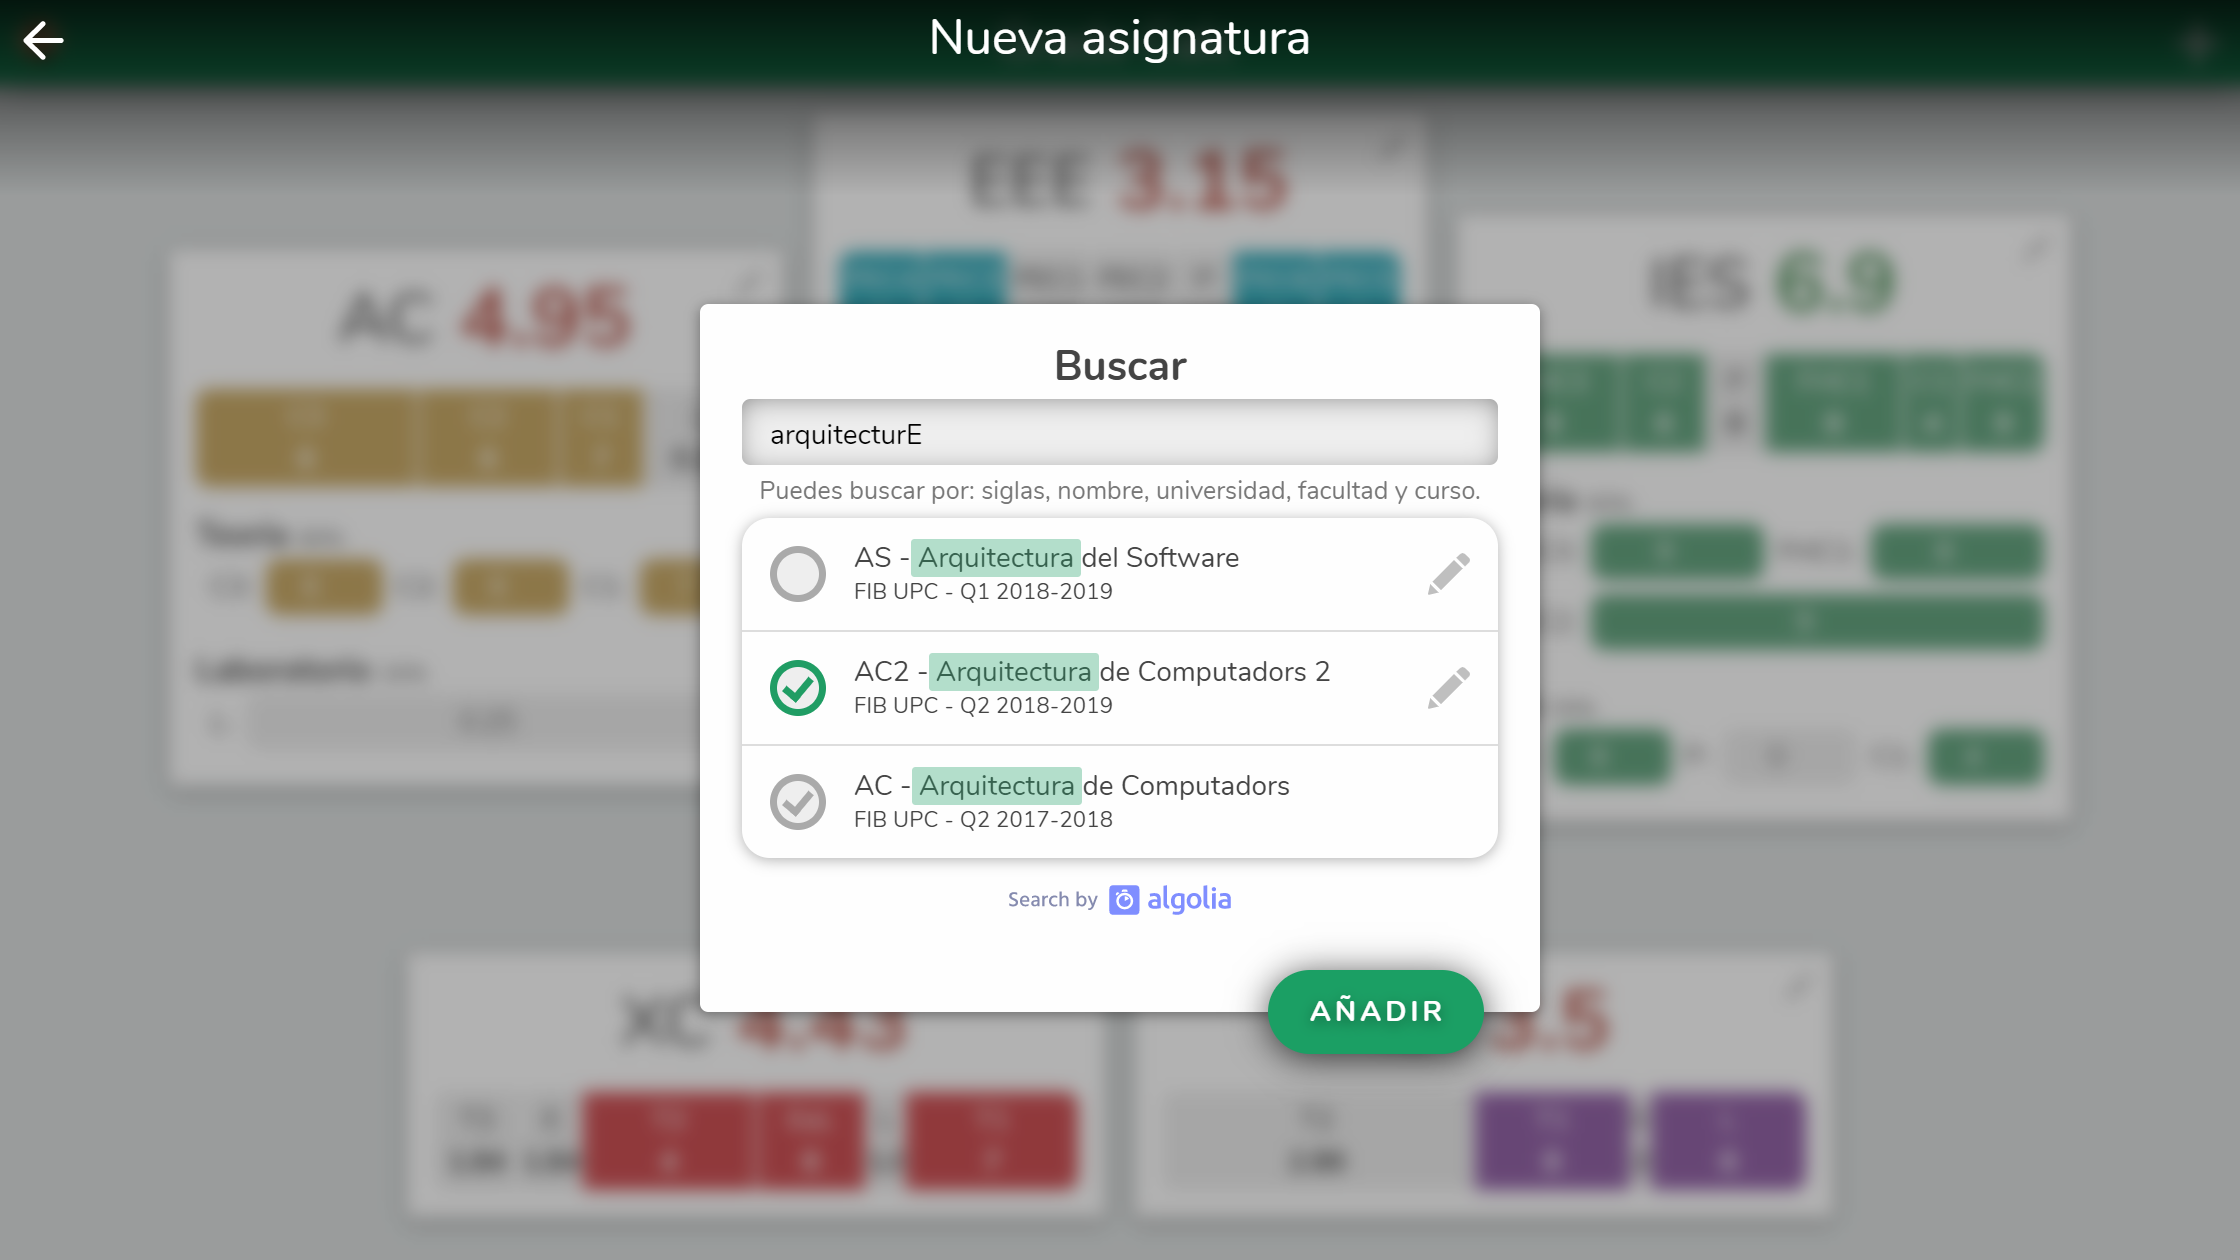
\includegraphics[width=\textwidth]{media/screenshots/screenshot-search-filled-pc.png}
        \caption{Desktop version}
    \end{subfigure}
    \hfill
    \begin{subfigure}[b]{0.243\textwidth-0.1cm}
        \centering
        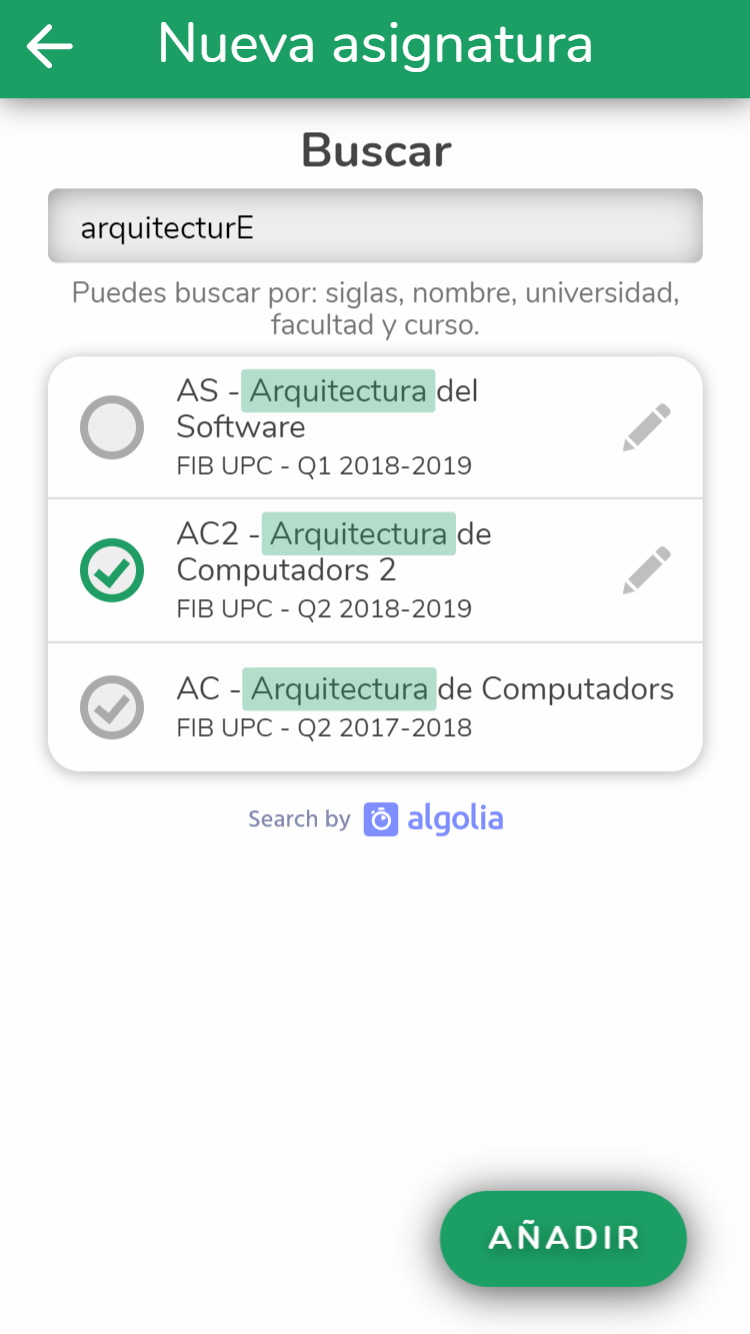
\includegraphics[frame,width=\textwidth]{media/screenshots/screenshot-search-filled.png}
        \caption{Mobile version}
    \end{subfigure}
    \caption{Search subjects input filled}
    \label{fig:search-filled}
\end{figure}
\vfill

\clearpage\newpage
If no results are matching the query a flashy test appears. If nothing is displayed the users think that it's loading or it doesn't work. 

The \inlineicon{button-create-gray.png} button hides if there are search results and shows back when there are not. The reasoning behind it is that if the student can't find a subject he'll have to inevitably create it, making it easier for him to find the button.

Algolia's community plan\cite{algolia-community-plan}, the free one, requires to place their logo close to the search results, so this is why the logo of the search engine is there.

\vfill
\begin{figure}[ht!]
    \begin{subfigure}[b]{0.757\textwidth-0.1cm}
        \centering
        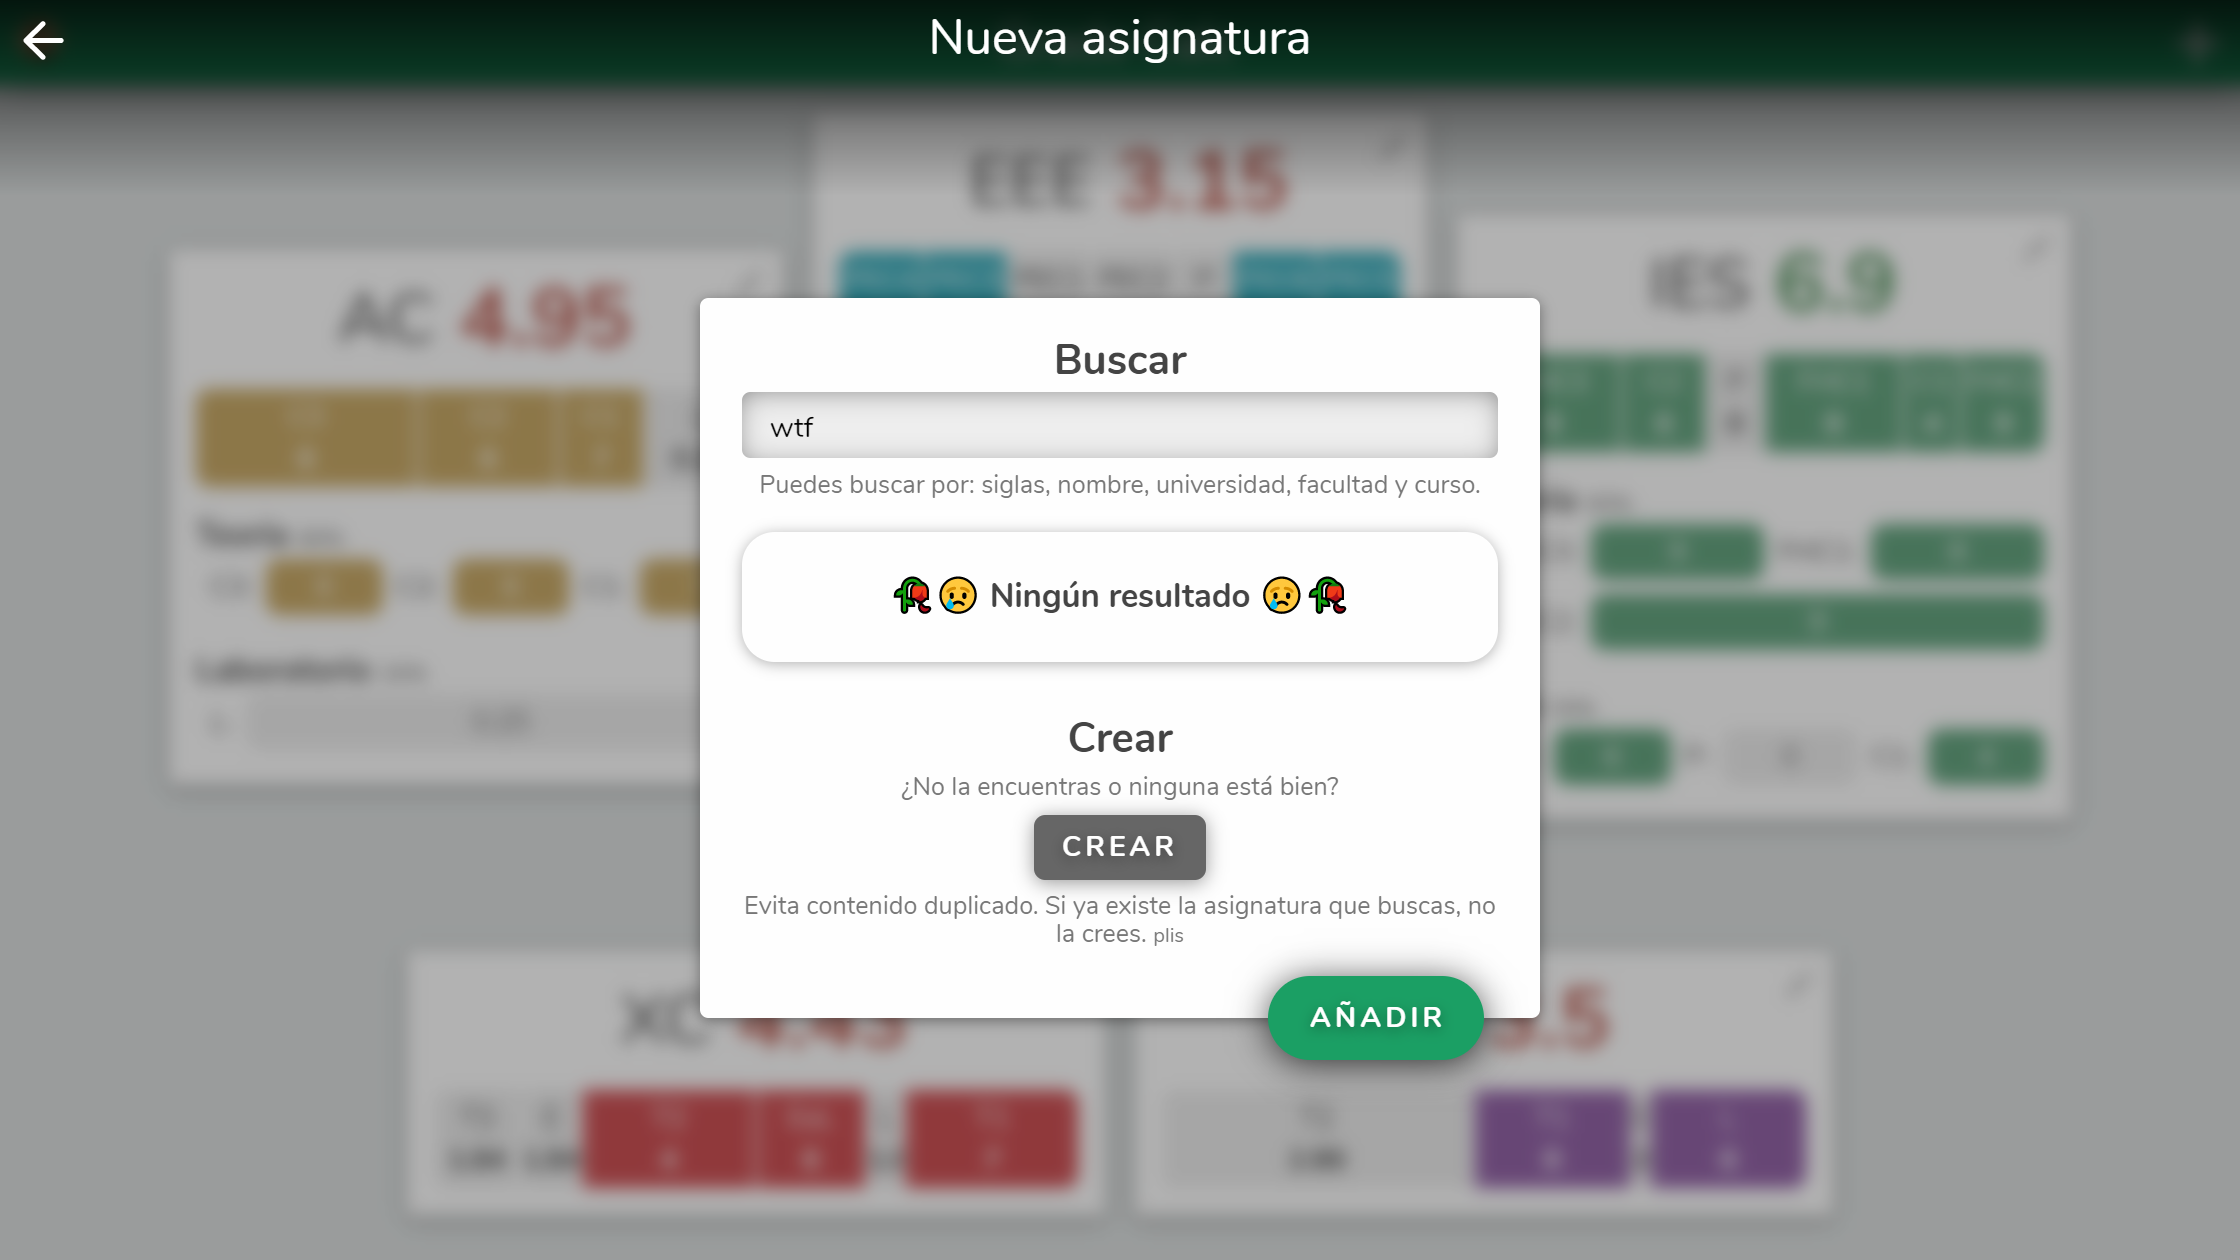
\includegraphics[width=\textwidth]{media/screenshots/screenshot-search-nothing-pc.png}
        \caption{Desktop version}
    \end{subfigure}
    \hfill
    \begin{subfigure}[b]{0.243\textwidth-0.1cm}
        \centering
        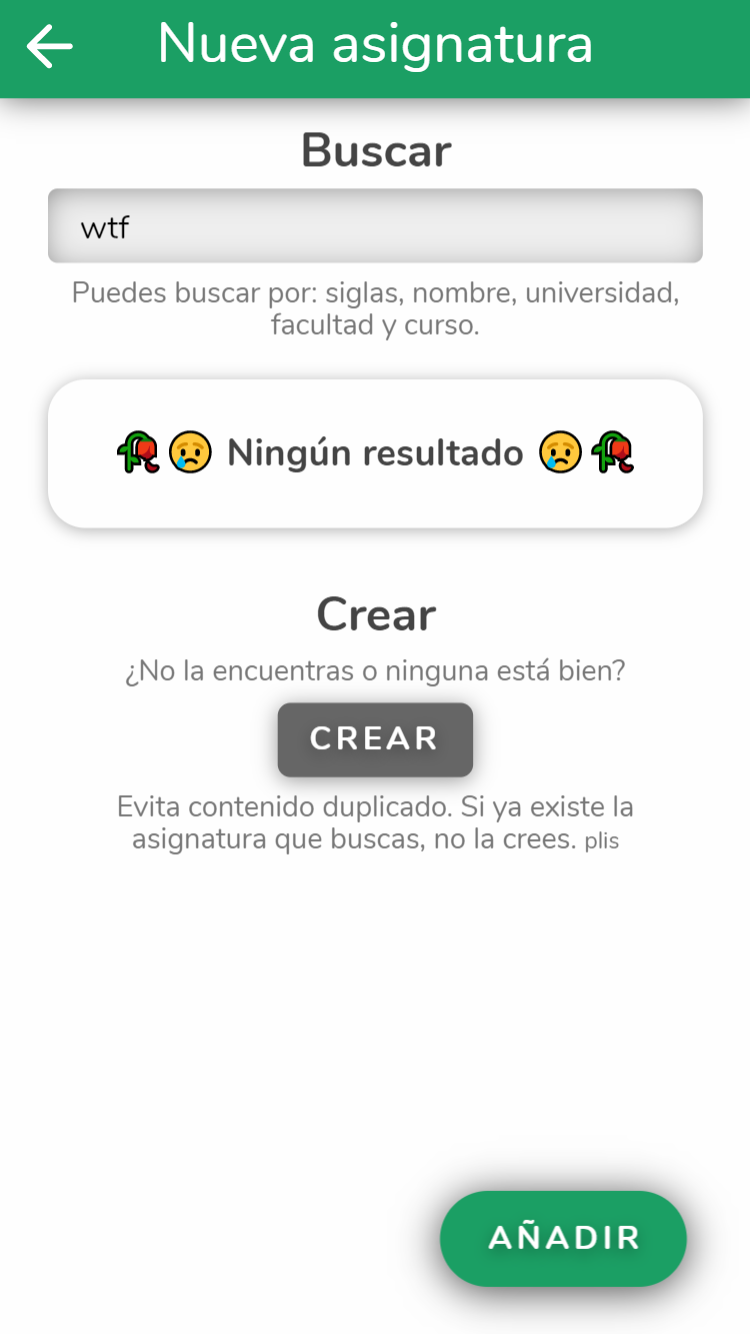
\includegraphics[frame,width=\textwidth]{media/screenshots/screenshot-search-nothing.png}
        \caption{Mobile version}
    \end{subfigure}
    \caption{No search results found}
    \label{fig:search-nothing}
\end{figure}
\vfill
% \begin{figure}[ht!]
%     \centering
%     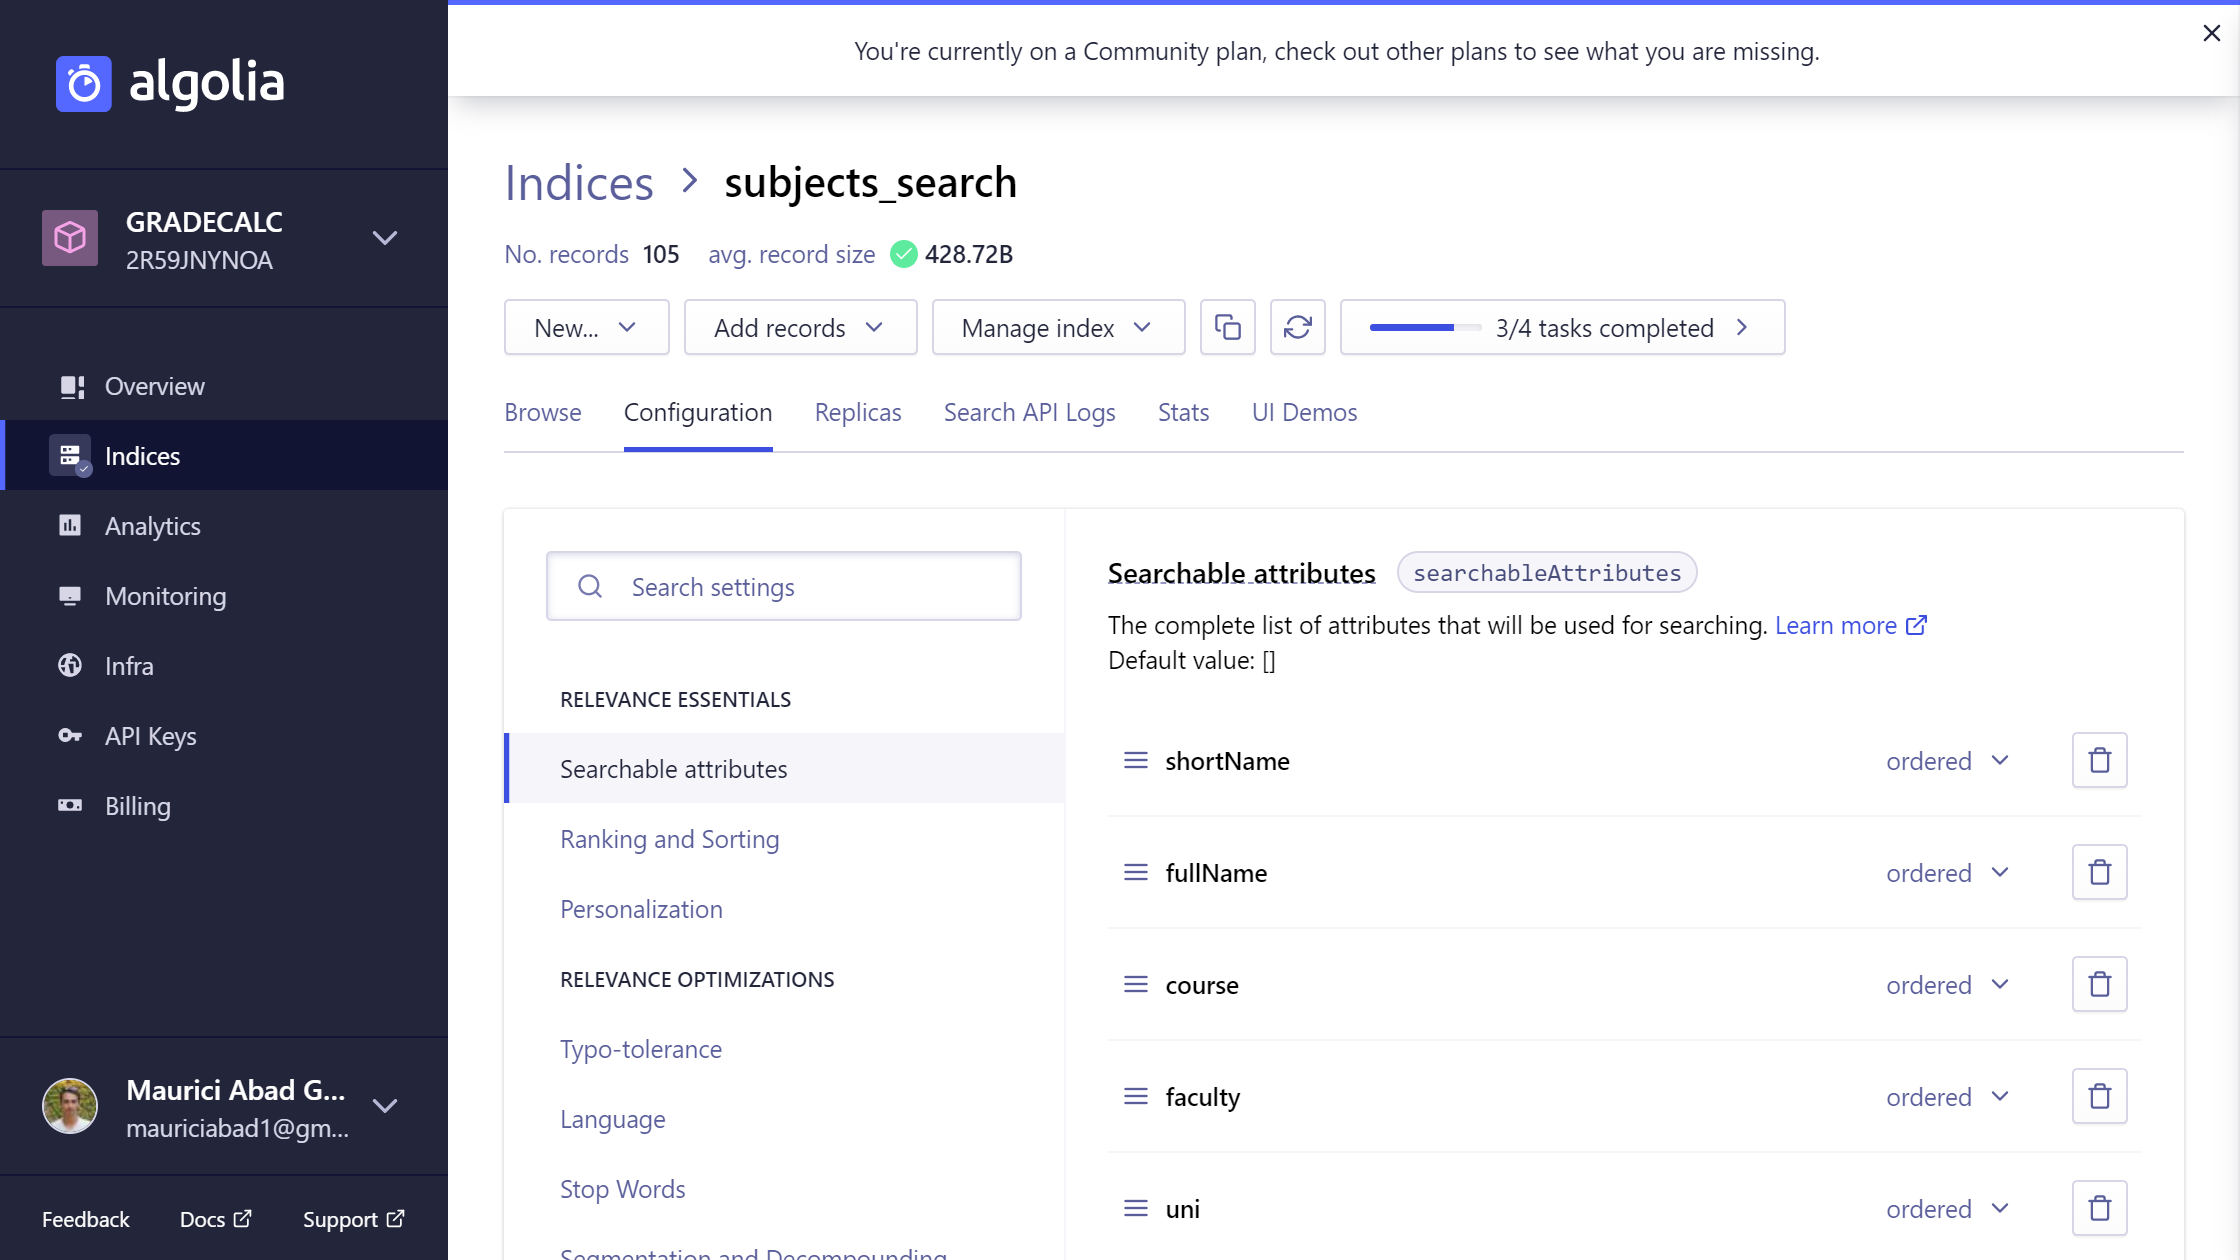
\includegraphics[width=0.75\textwidth]{media/algolia-dashboard.png}
%     \caption{Algolia index settings for GradeCalc}
%     \label{fig:algolia-dashboard}
% \end{figure}
% \vfill


\clearpage\newpage
\subsubsection{Edit and create subject}

When the \inlineicon{icon-edit.pdf} button is clicked, ether from the subject card (Fig. \ref{fig:card}) or the search result (Fig. \ref{fig:card}) this screen is opened. 
% Here the fields \textit{shortName}, \textit{longName}, \textit{course}, \textit{faculty}, \textit{university} and \textit{color} can be edited. 
The evaluation can be edited using the grid on the bottom.

In the grid, each row is a different exam. And this is what every column represents:
\begin{itemize}[itemsep=0mm]
    \item The first column holds the name of the exam.
    \item The second column holds the name of the type of the exam, this is only used to better organize exams inside the subject card (Fig. \ref{fig:card}).
    \item The third column holds the initial value of the exam. The usual is to leave it empty.
    \item Every additional column represents a different evaluation. The first cell is the name of the evaluation and the rest cells are the weight of the exam over 100.
\end{itemize}
Conveniently at the bottom of each evaluation column, there's the sum of all values of the column, to make sure they add up to 100\% exactly and avoid mistakes. 

To create new rows and columns just type in the faded cells, and to delete a row or column, just empty all of its values and it will disappear.


\vfill
\begin{figure}[ht!]
    \begin{subfigure}[b]{0.757\textwidth-0.1cm}
        \centering
        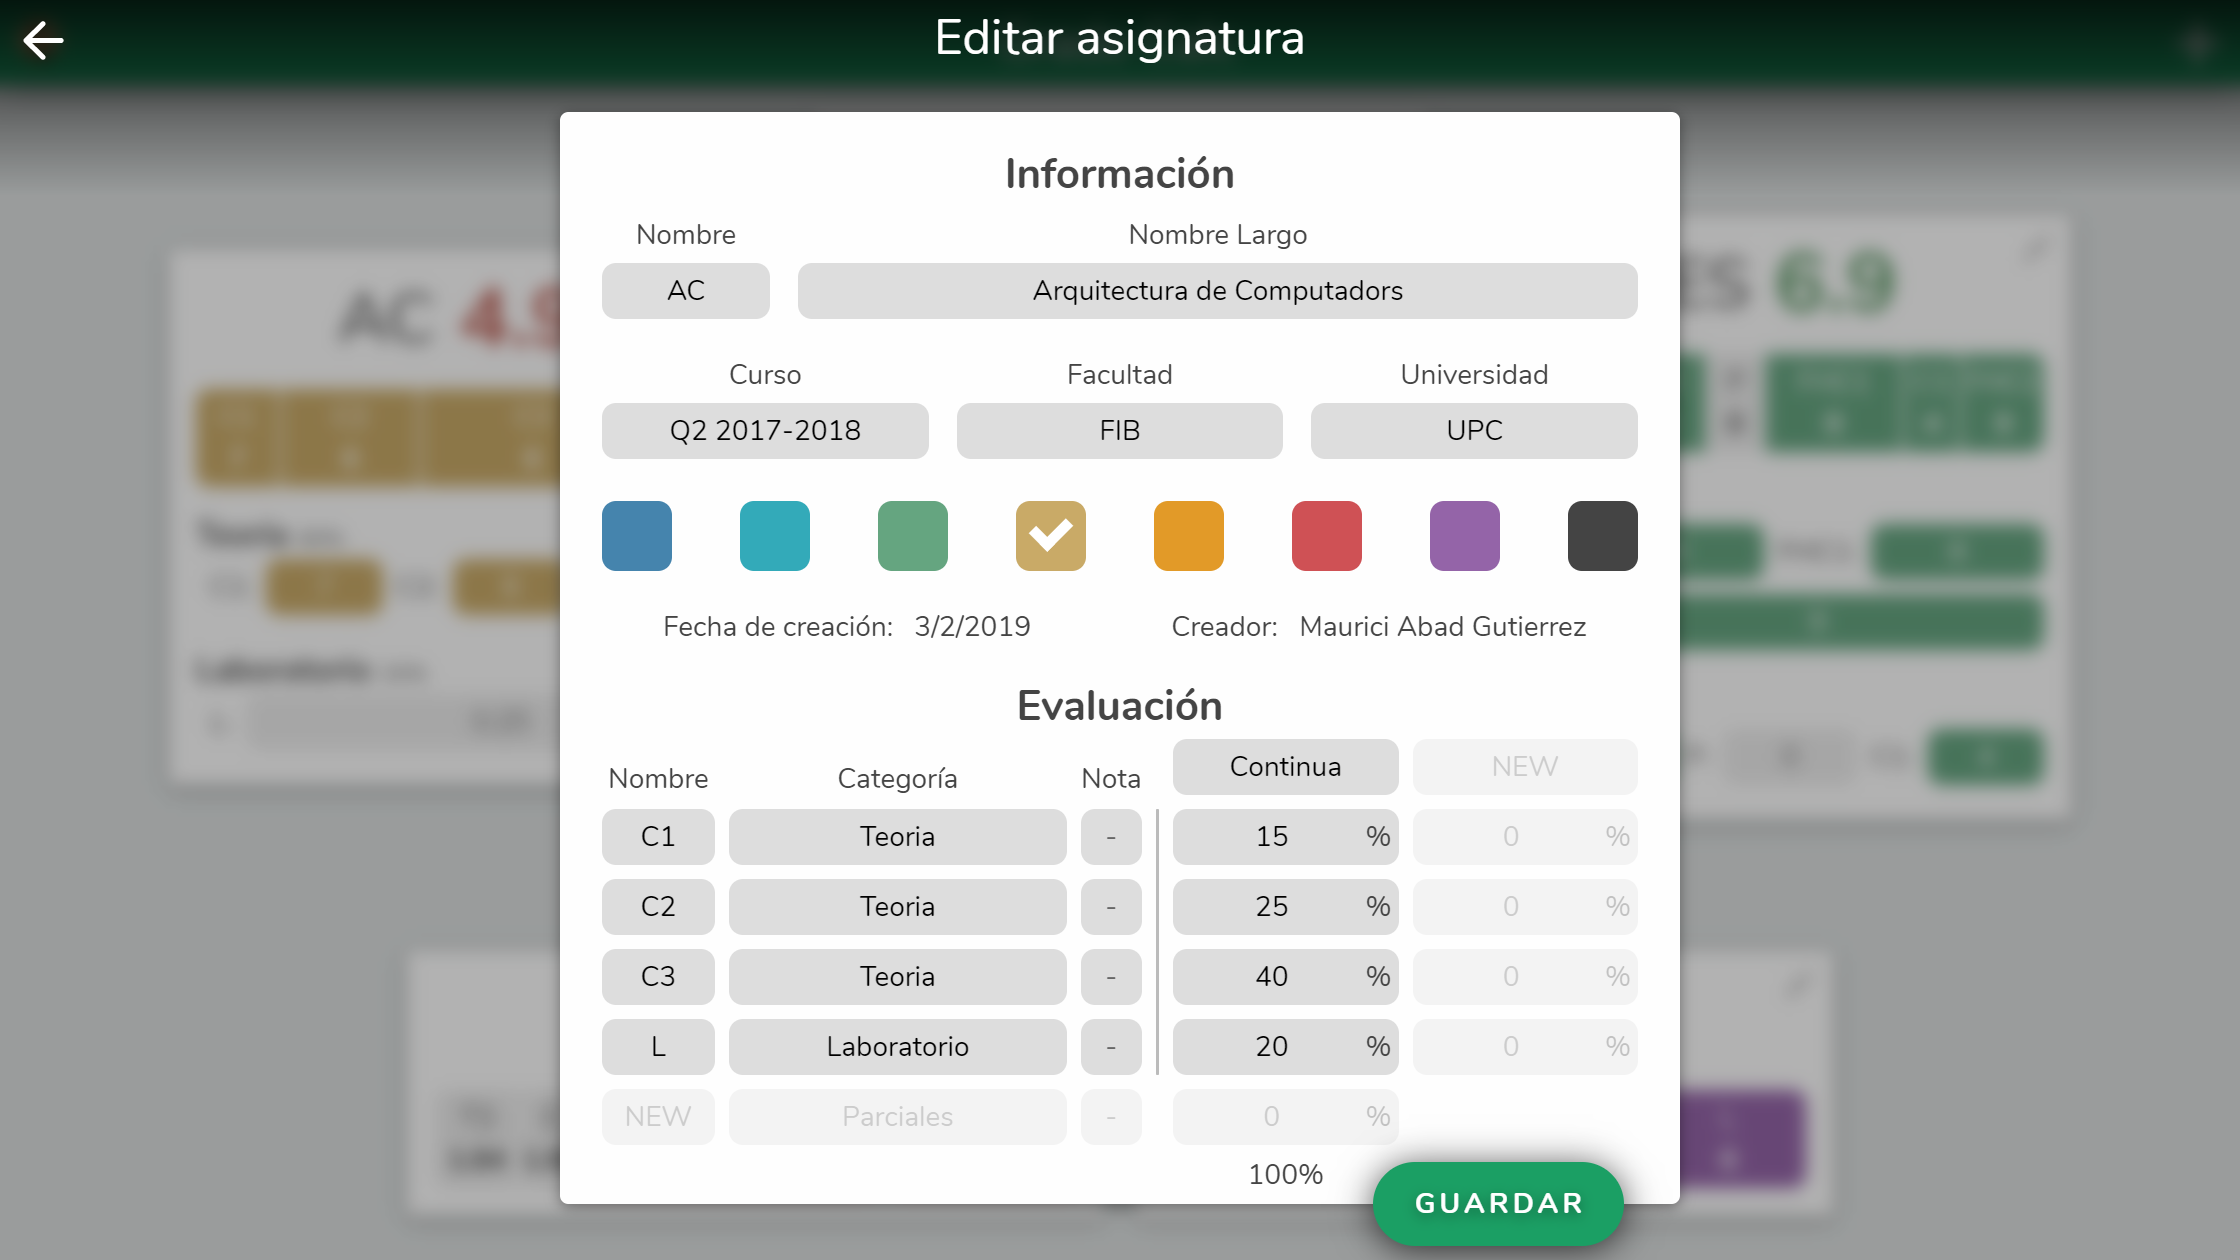
\includegraphics[width=\textwidth]{media/screenshots/screenshot-edit-pc.png}
        \caption{Desktop version}
    \end{subfigure}
    \hfill
    \begin{subfigure}[b]{0.243\textwidth-0.1cm}
        \centering
        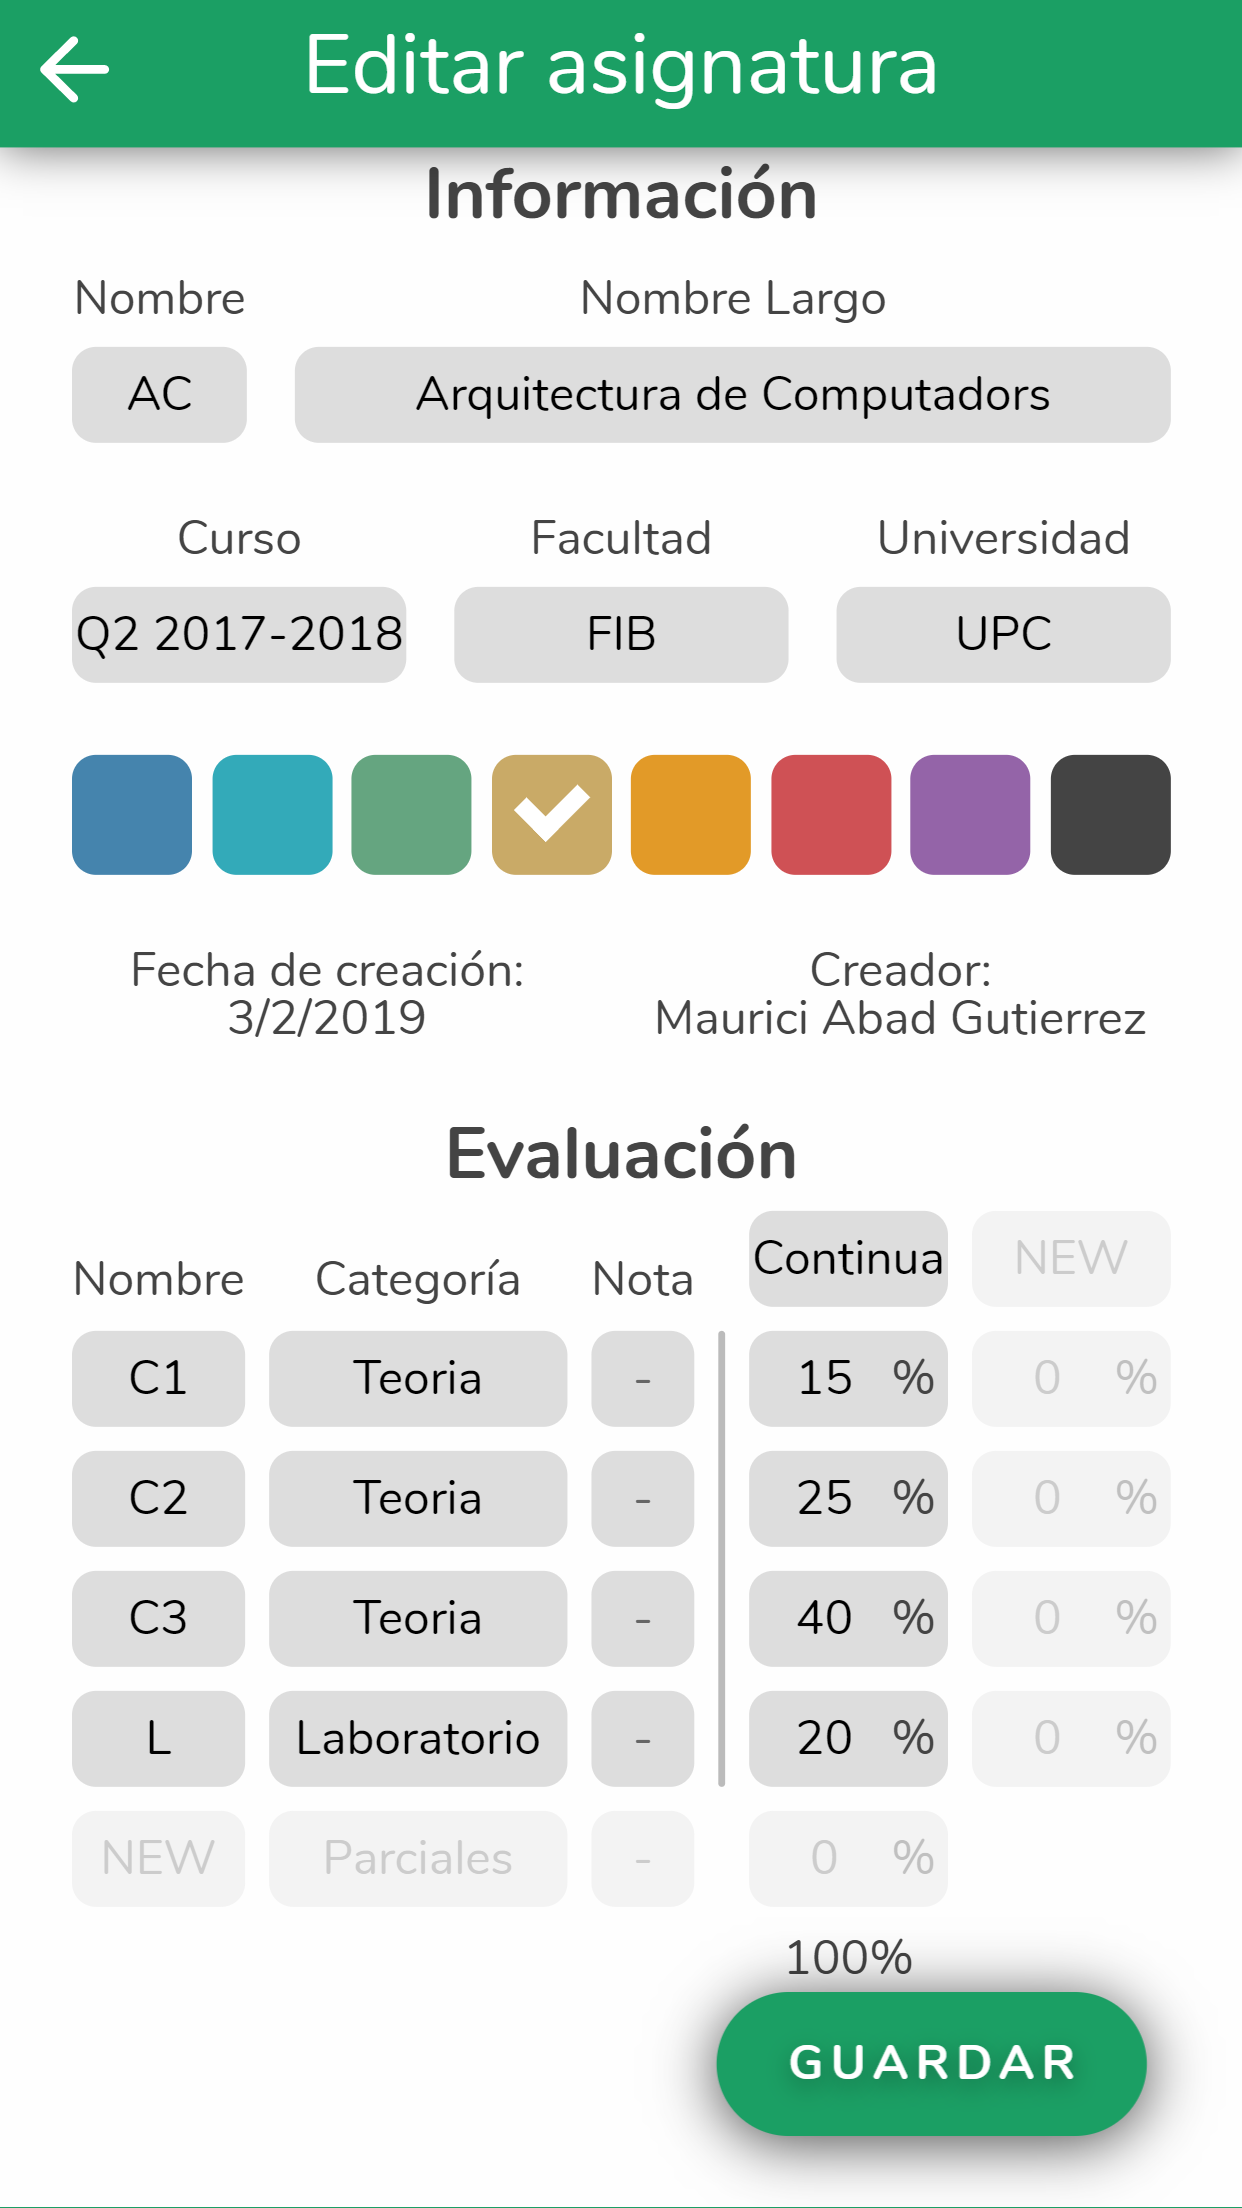
\includegraphics[frame,width=\textwidth]{media/screenshots/screenshot-edit.png}
        \caption{Mobile version}
    \end{subfigure}
    \caption{Edit subject}
    \label{fig:edit}
\end{figure}
\vfill

\clearpage\newpage

When creating a new subject by clicking the \inlineicon{button-create-gray.png} button this screen is also open, but its content is empty. As shown in Figure \ref{fig:create}, there's a validation on the inputs, none of them can be empty, that's why they have a red border. If the user tries to create or edit the subject by pressing the \inlineicon{button-create.png} or \inlineicon{button-save.png} button a notification will pop up describing the error (Fig. \ref{fig:notifications}). Another validation made is that there must be at least one evaluation and one exam.

Once the user clicks the \inlineicon{button-create.png} button, a blocking spinner (Fig. \ref{fig:freeze}) will show because creating the record takes approximately between 0.5s to 2s. Otherwise, users would click the button several times, generating many duplicates. It also lets them know that the app is loading.

\vfill
\begin{figure}[ht!]
    \begin{subfigure}[b]{0.757\textwidth-0.1cm}
        \centering
        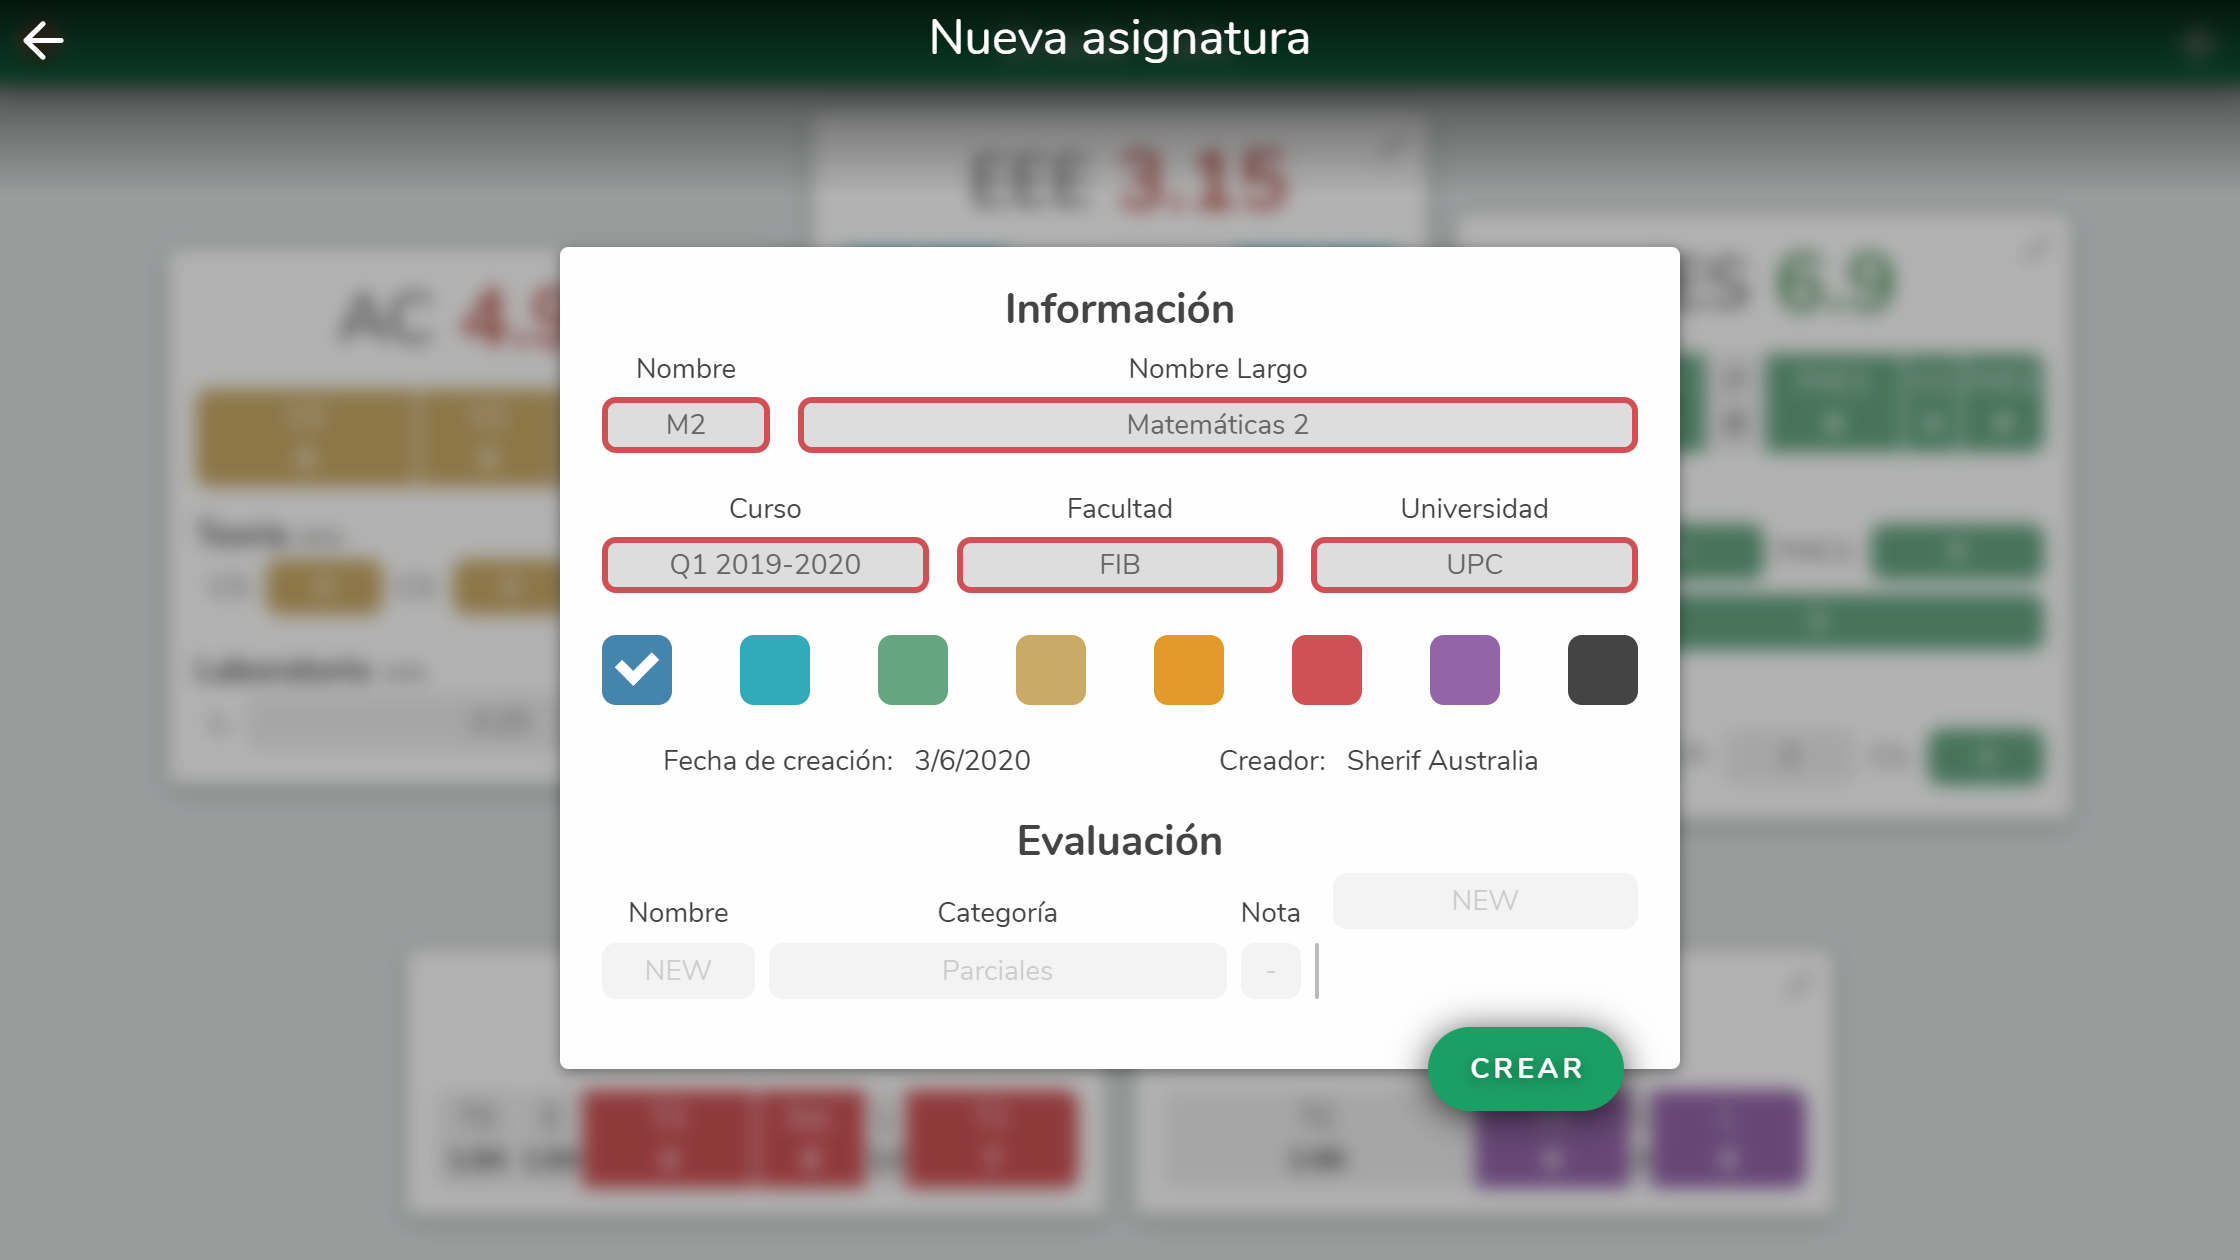
\includegraphics[width=\textwidth]{media/screenshots/screenshot-create-pc.png}
        \caption{Desktop version}
    \end{subfigure}
    \hfill
    \begin{subfigure}[b]{0.243\textwidth-0.1cm}
        \centering
        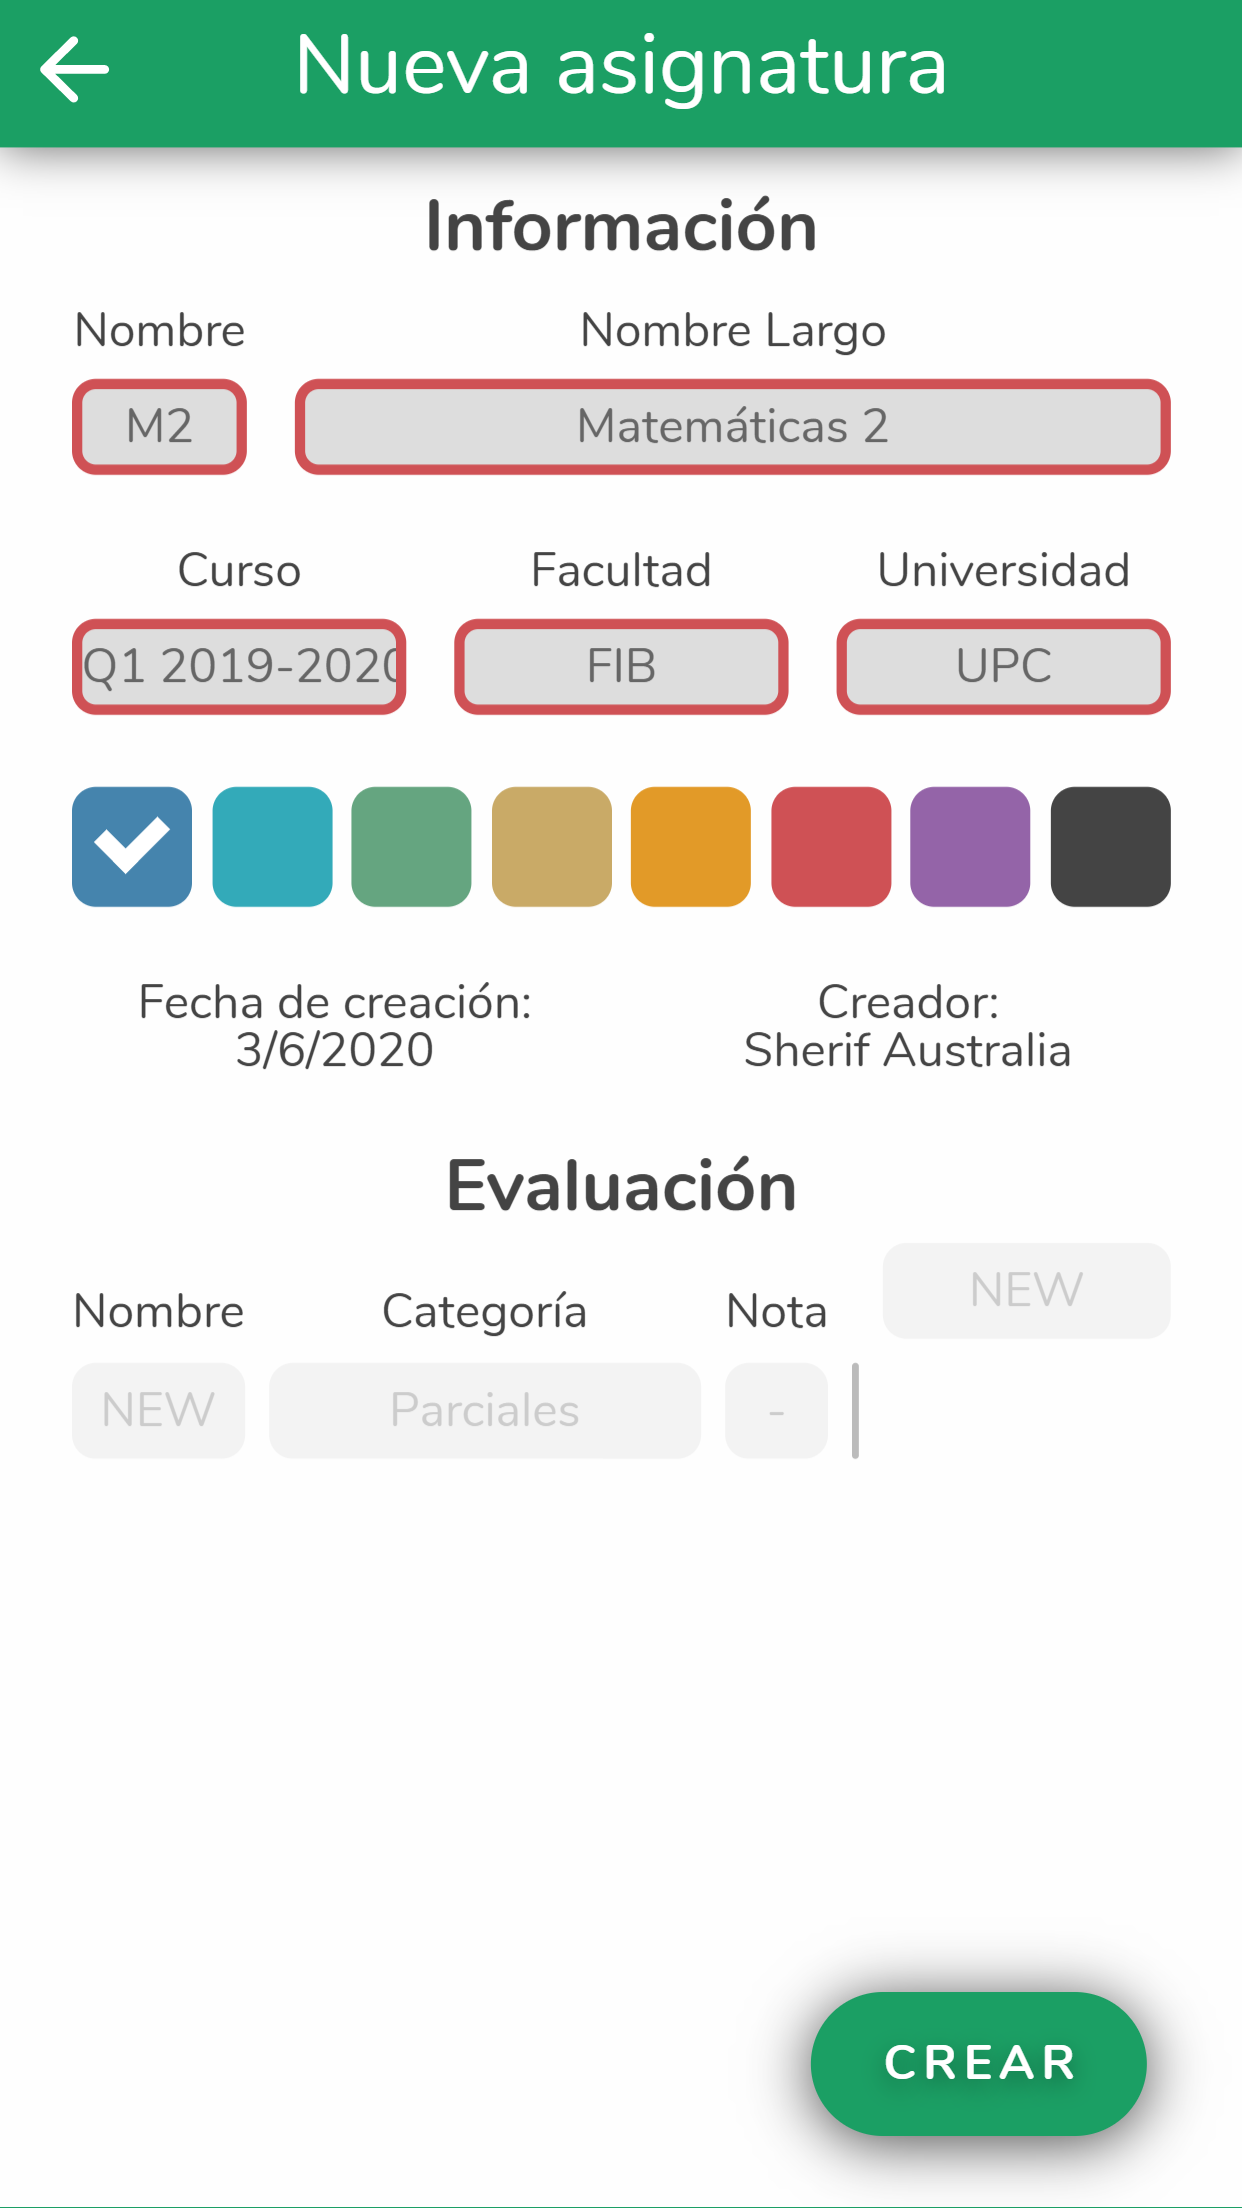
\includegraphics[frame,width=\textwidth]{media/screenshots/screenshot-create.png}
        \caption{Mobile version}
    \end{subfigure}
    \caption{Create subject}
    \label{fig:create}
\end{figure}
\vfill

\clearpage\newpage
\subsubsection{Log-in and log-out}

The login screen is the simplest one, it's just a popup in the desktop and mobile, it has a profile picture, name, description of the benefits of logging in and the log-in \inlineicon{button-login.png} button or log-out \inlineicon{button-logout.png} button. It's opened when the \inlineicon{icon-user.pdf} button is clicked.

Then the user is not logged, the profile picture is a placeholder one, and the name is \textit{Anonymous}.

Clicking the \inlineicon{button-login.png} button goes to Google's log-in page (Fig. \ref{fig:login-google}) where the student picks his account and then he's redirected to GradeCalc again.

To log-out, the user just has to open the popup and click the \inlineicon{button-logout.png} button.

When the user logins the subjects that he had on the dashboard are synced to the ones in his account. For example, if he added a grade from the mobile and opens the app on the laptop the changes will be downloaded.

\vfill
\begin{figure}[ht!]
    \begin{subfigure}[b]{0.757\textwidth-0.1cm}
        \centering
        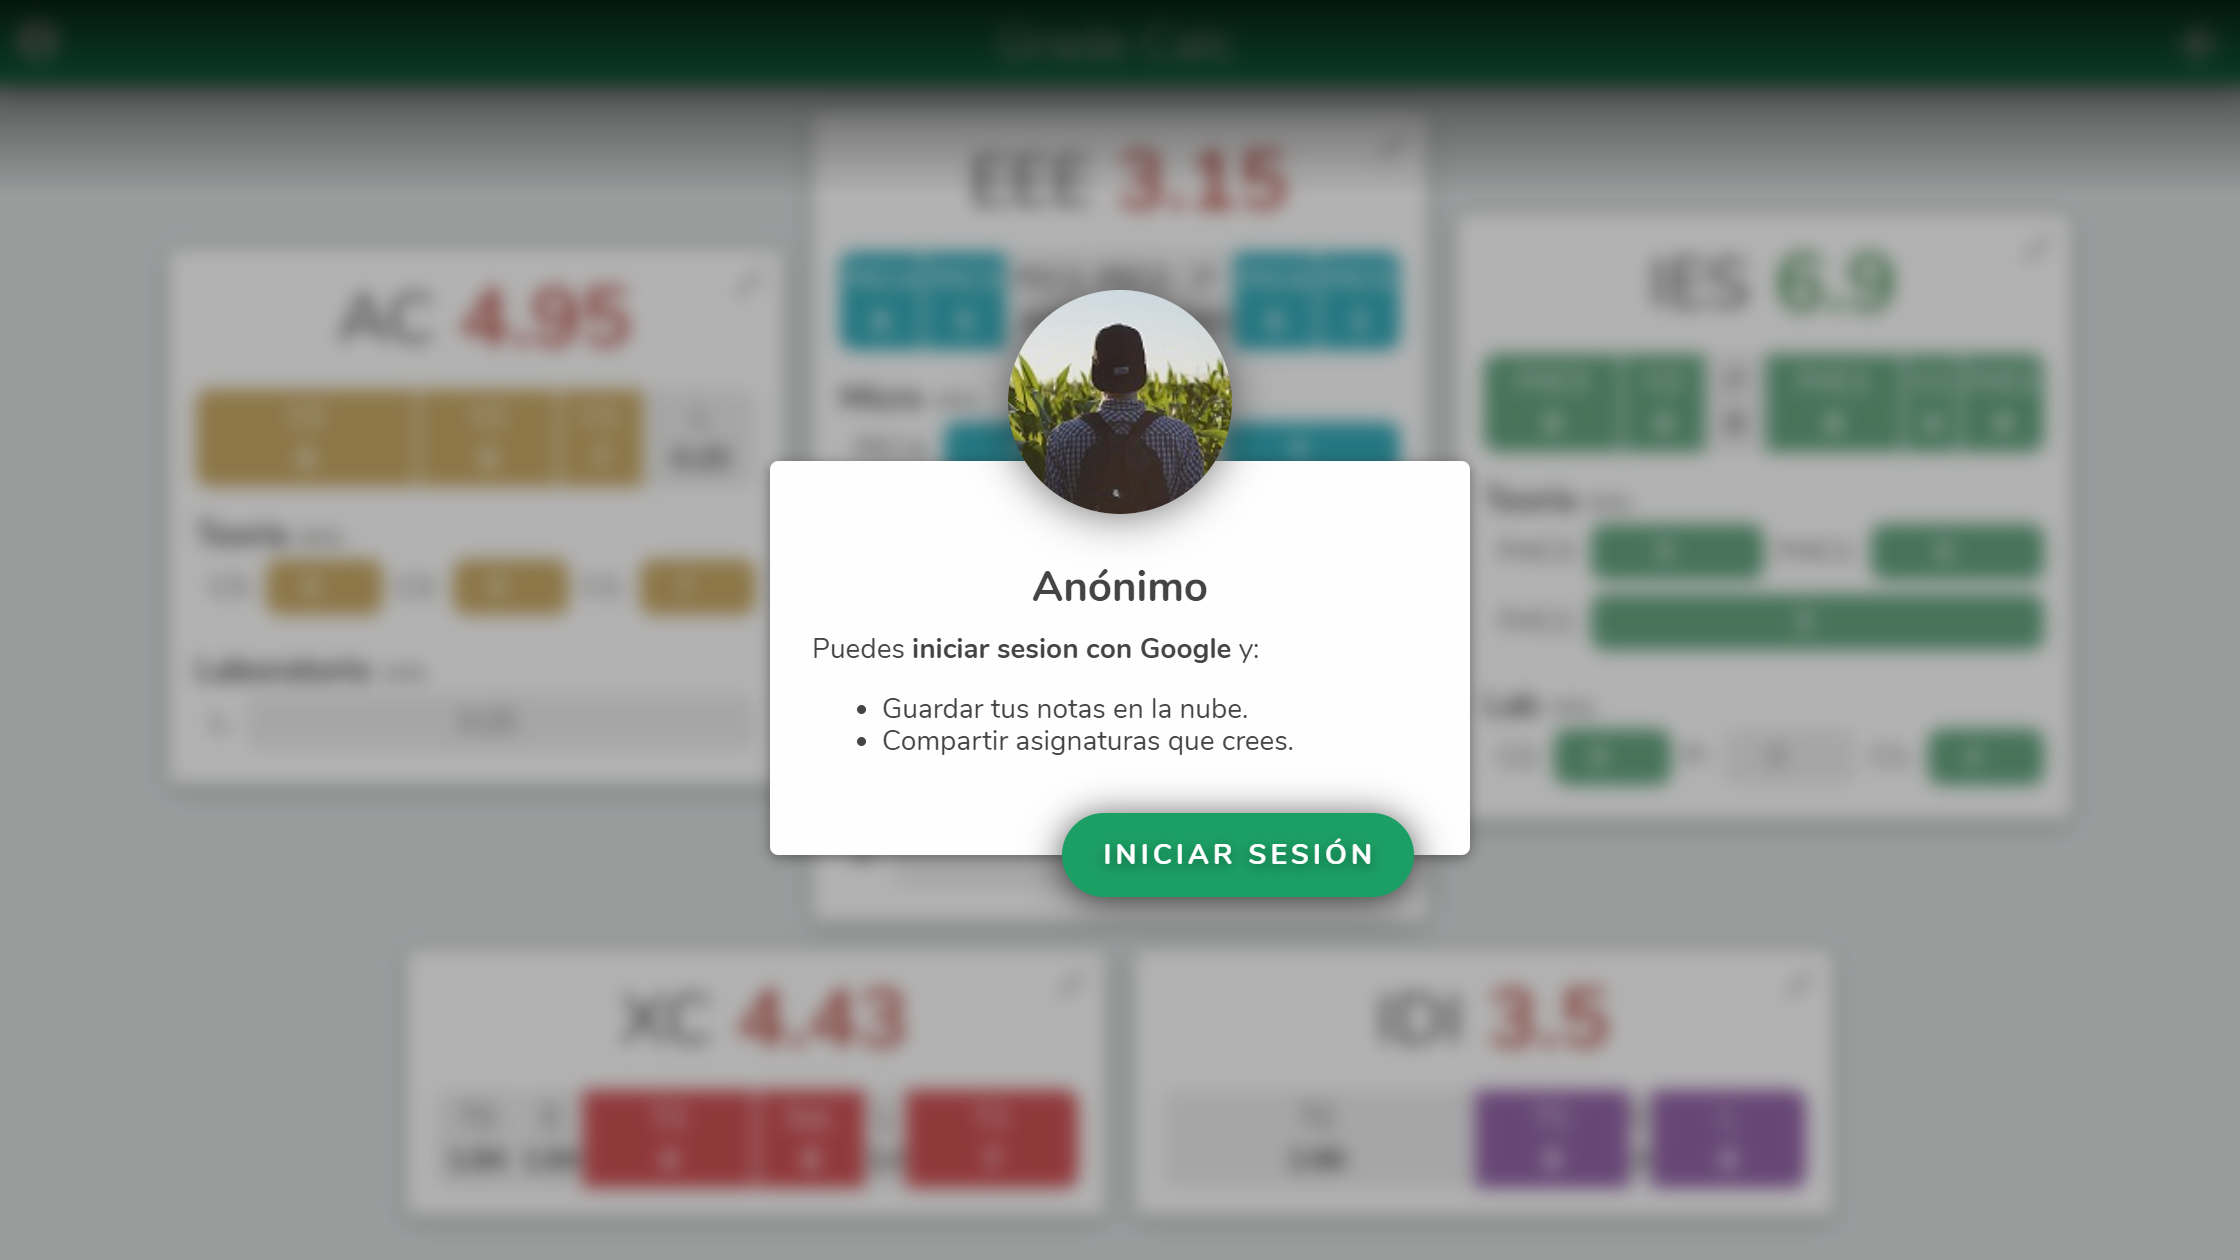
\includegraphics[width=\textwidth]{media/screenshots/screenshot-login-pc.png}
        \caption{Desktop version}
    \end{subfigure}
    \hfill
    \begin{subfigure}[b]{0.243\textwidth-0.1cm}
        \centering
        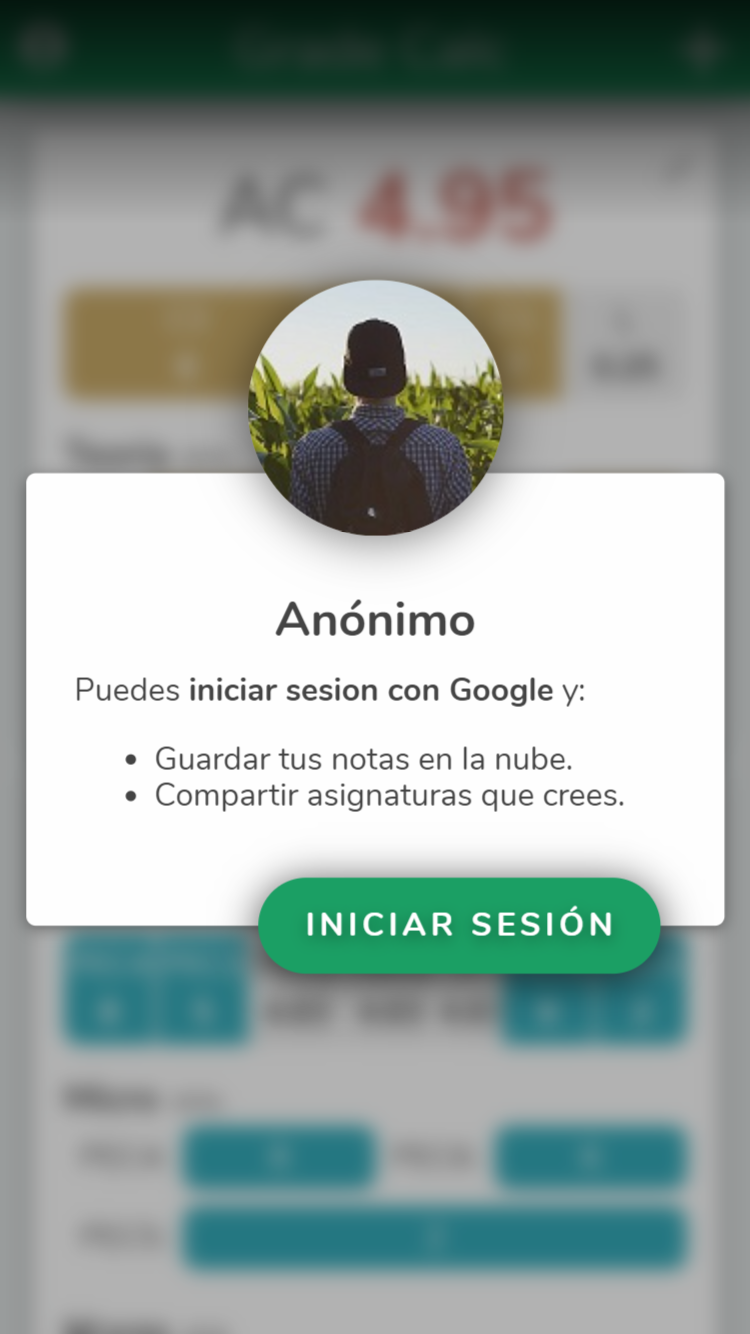
\includegraphics[width=\textwidth]{media/screenshots/screenshot-login.png}
        \caption{Mobile version}
    \end{subfigure}
    \caption{Log-in user is not logged in}
    \label{fig:login}
\end{figure}
\vfill

\clearpage\newpage

\vfill
\begin{figure}[ht!]
    \begin{subfigure}[b]{0.757\textwidth-0.1cm}
        \centering
        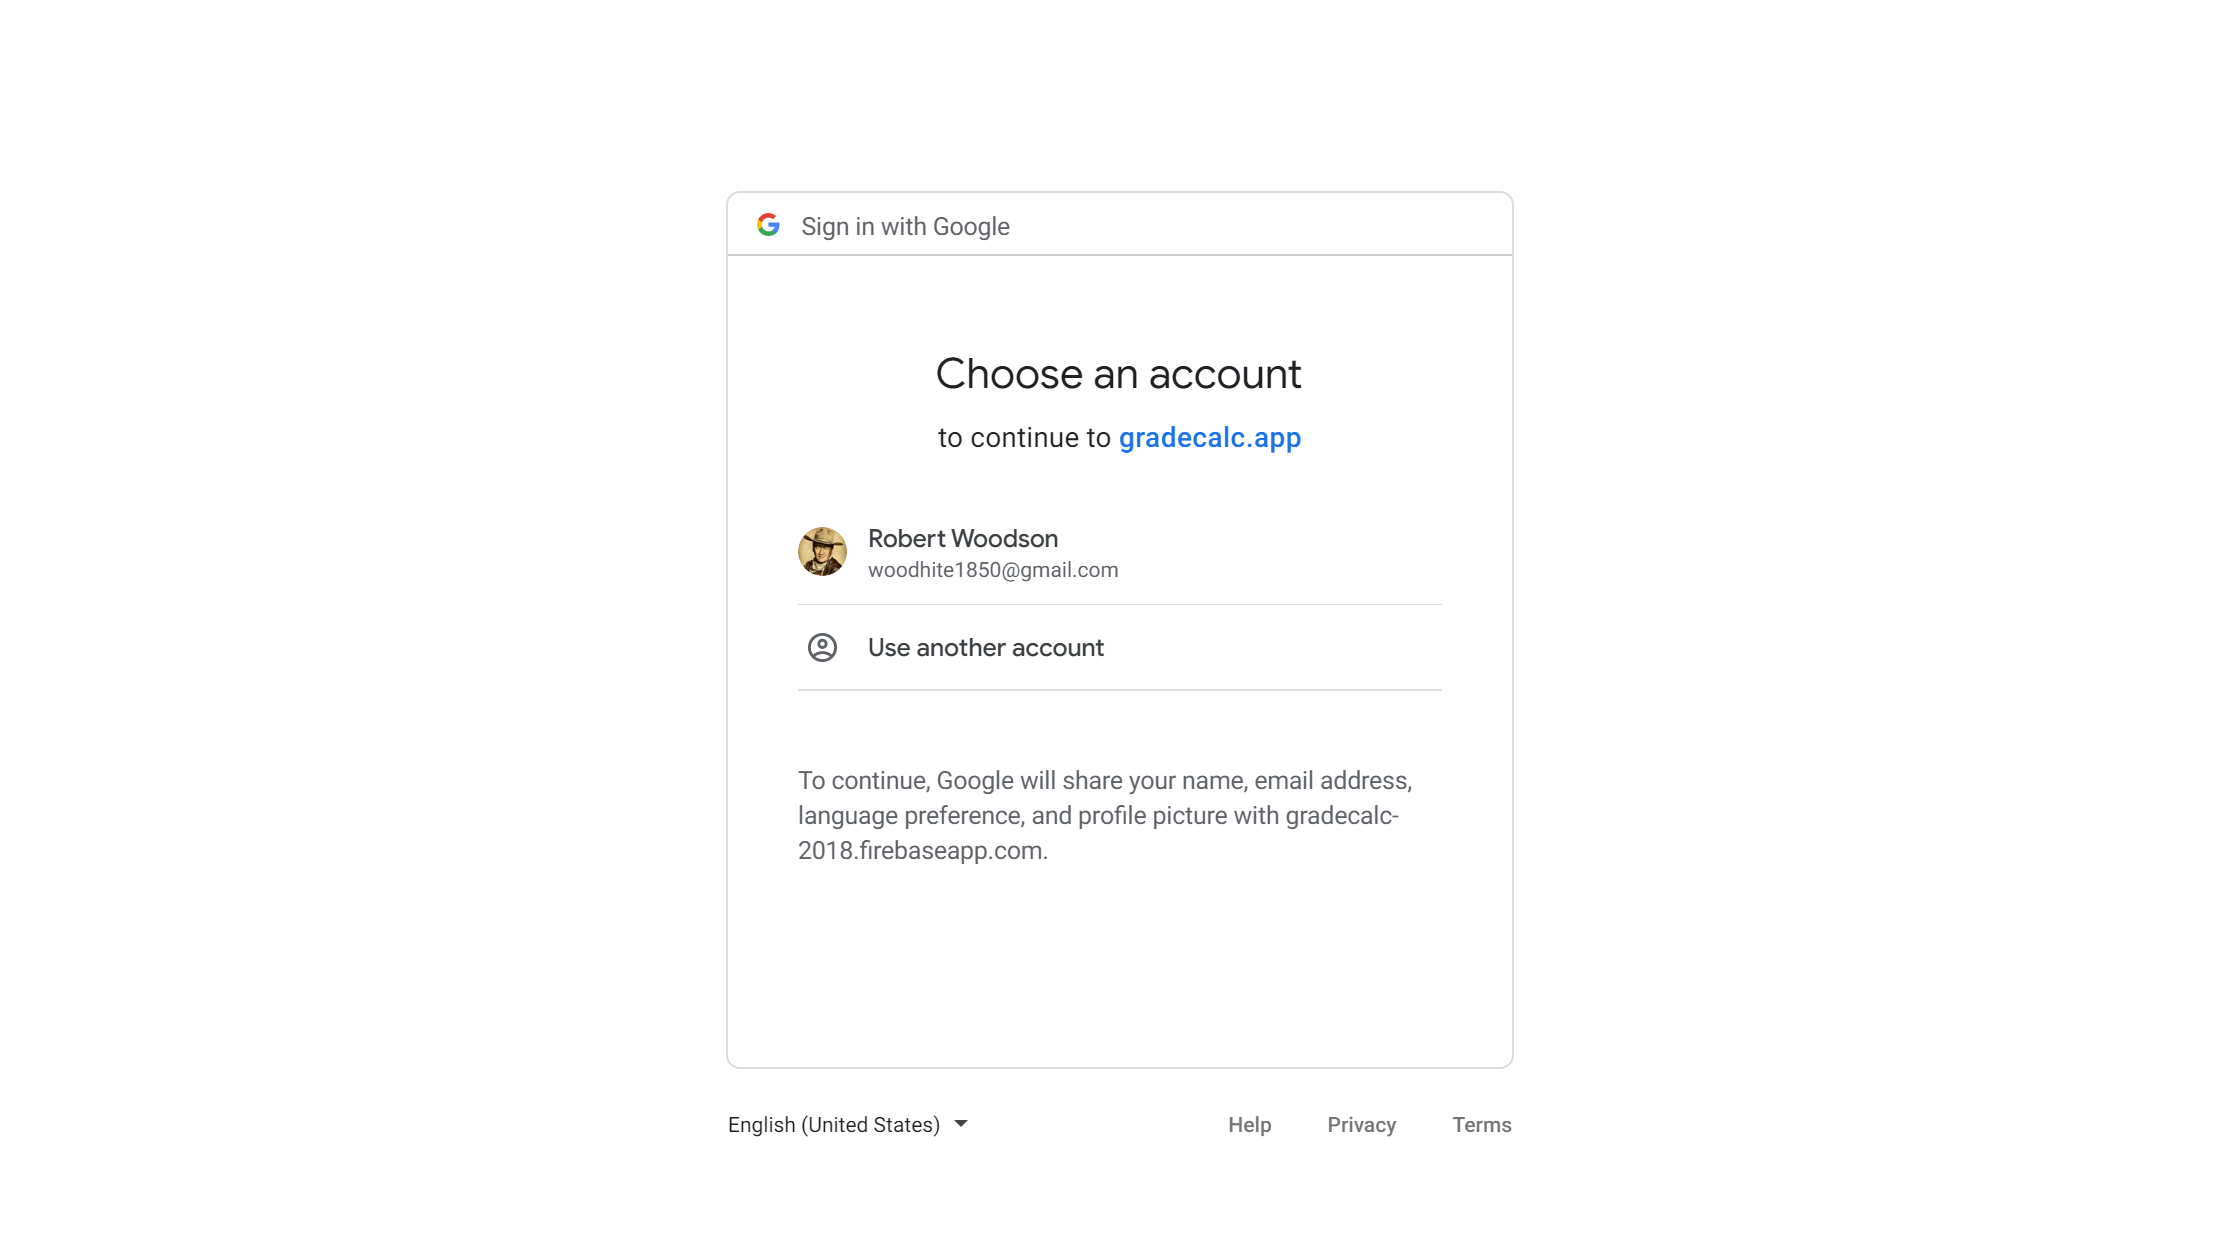
\includegraphics[frame,width=\textwidth]{media/screenshots/screenshot-login-google-pc.png}
        \caption{Desktop version}
    \end{subfigure}
    \hfill
    \begin{subfigure}[b]{0.243\textwidth-0.1cm}
        \centering
        
\includegraphics[frame,width=\textwidth]{media/screenshots/screenshot-login-google.png}
        \caption{Mobile version}
    \end{subfigure}
    \caption{Log-in with google}
    \label{fig:login-google}
\end{figure}

\vfill

\begin{figure}[ht!]
    \begin{subfigure}[b]{0.757\textwidth-0.1cm}
        \centering
        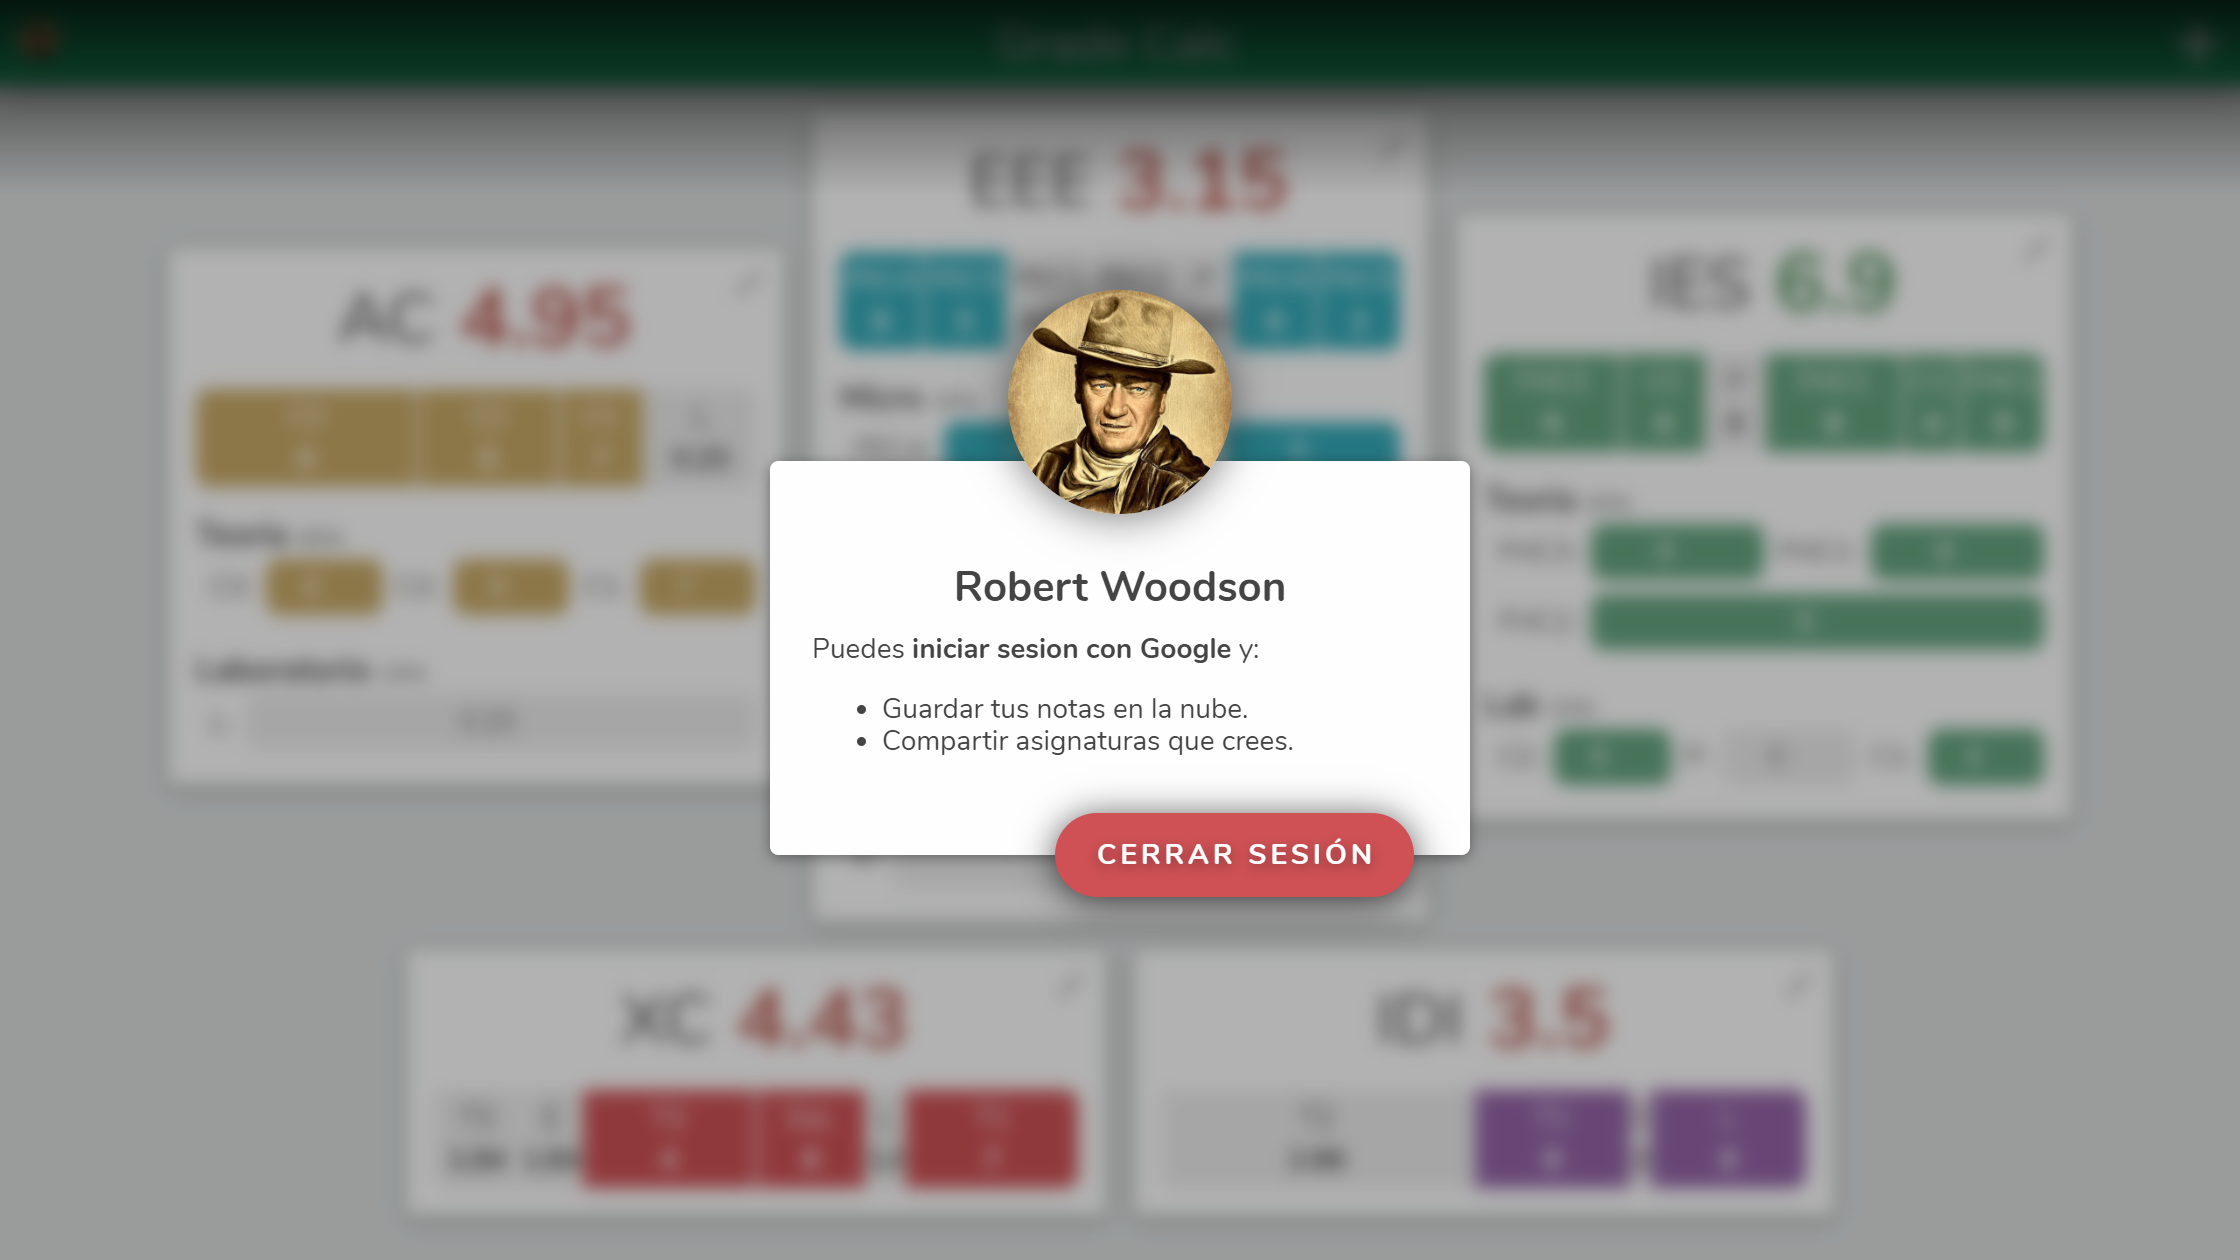
\includegraphics[width=\textwidth]{media/screenshots/screenshot-login-logout-pc.png}
        \caption{Desktop version}
    \end{subfigure}
    \hfill
    \begin{subfigure}[b]{0.243\textwidth-0.1cm}
        \centering
        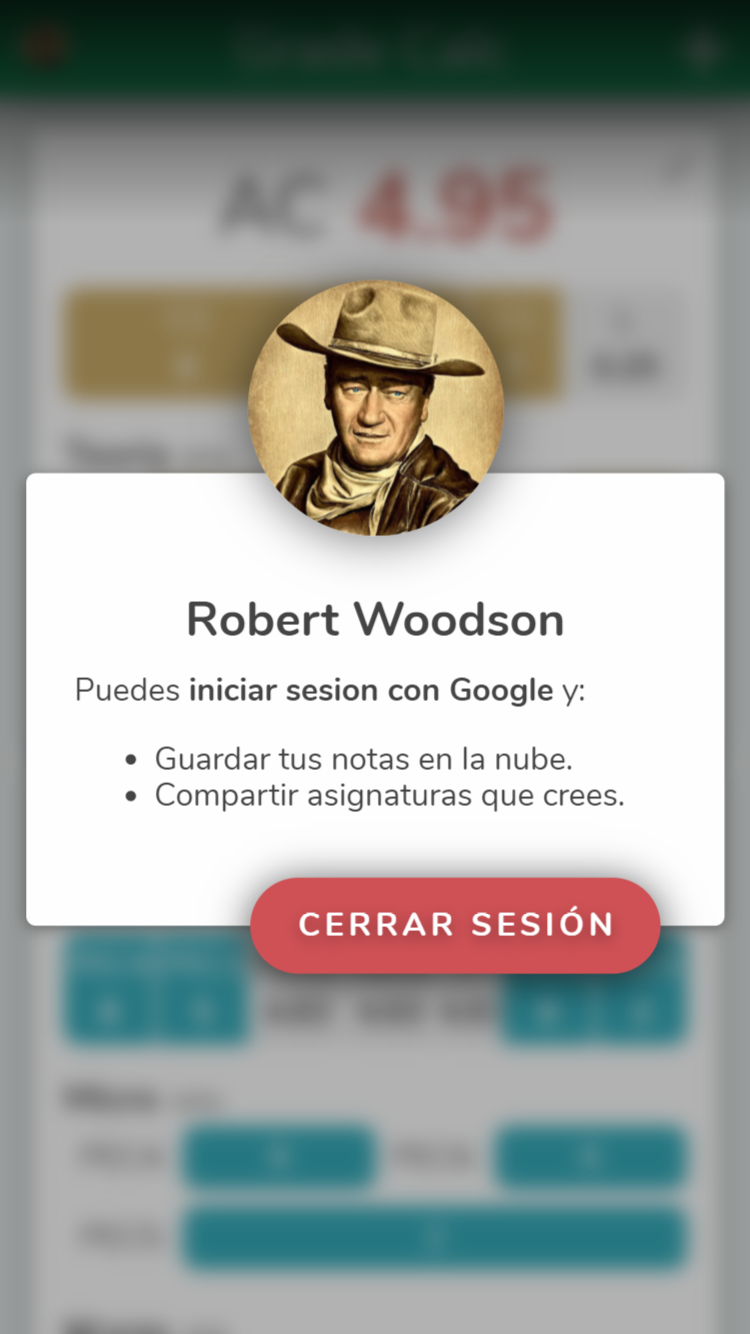
\includegraphics[width=\textwidth]{media/screenshots/screenshot-login-logout.png}
        \caption{Mobile version}
    \end{subfigure}
    \caption{Log-in user is logged in}
    \label{fig:login-logout}
\end{figure}
\vfill

% \clearpage\newpage
% \subsubsection{Other components}
% Some of the elements of the app appear on several screens. These are the components that are reused over the application.

\clearpage\newpage
\subsubsection{Background tasks spinner}

This component is a spinner for background tasks, that informs the user that a background process is happening, but lets him continue using the app. It appears at the bottom of the dashboard and its a bit faded to not be distracting.

In the examples bellow (Fig. \ref{fig:spinner}) we can see the three most common messages:
\begin{enumerate}[label=\textbf{(\alph*)},noitemsep]
    \item \textbf{Loading}: Getting subjects from the device's local storage.
    \item \textbf{Searching}: Logging-in and connecting to the database.
    \item \textbf{Downloading}: Getting subjects from user's account in the database.
\end{enumerate}

\vfill
\begin{figure}[ht!]
    \begin{subfigure}[b]{0.3333\textwidth-0.1cm}
        \centering
        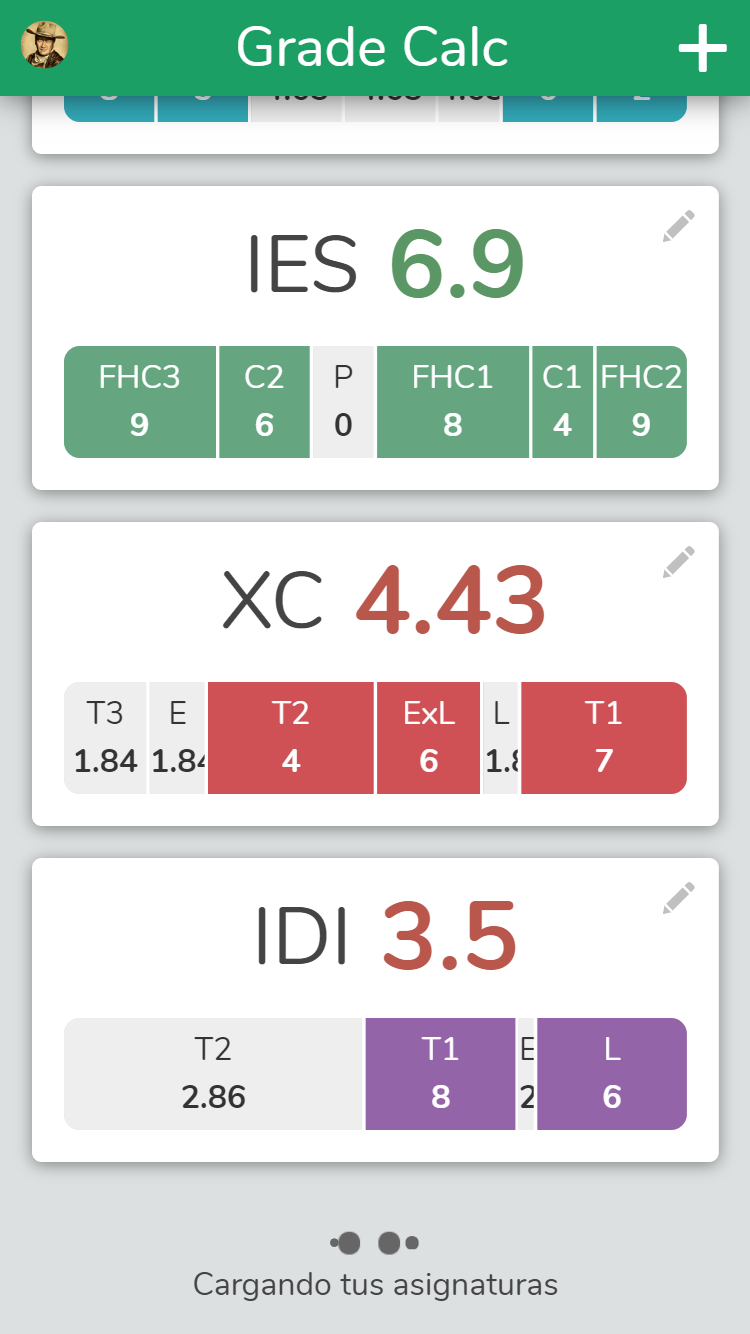
\includegraphics[width=\textwidth]{media/screenshots/screenshot-loader-cargando.png}
        \caption{Loading}
    \end{subfigure}
    \hfill
    \begin{subfigure}[b]{0.3333\textwidth-0.1cm}
        \centering
        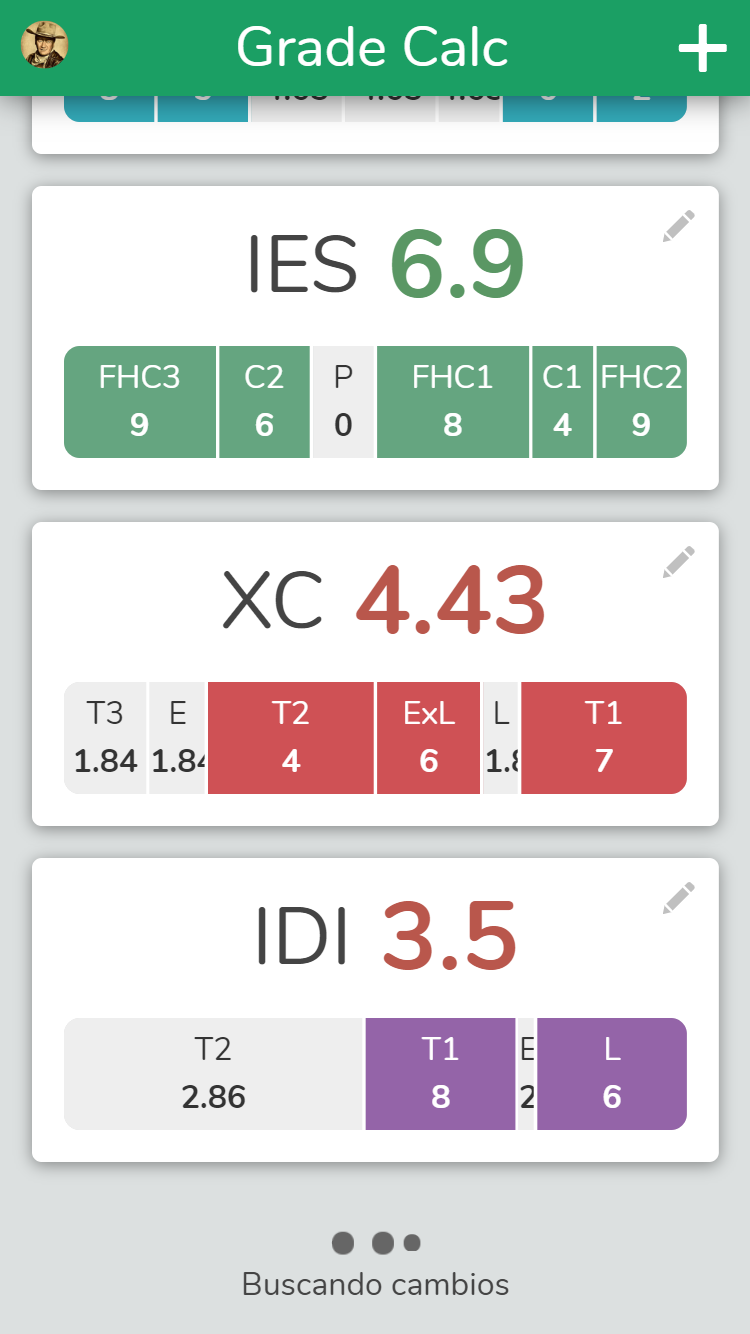
\includegraphics[width=\textwidth]{media/screenshots/screenshot-loader-buscando.png}
        \caption{Searching}
    \end{subfigure}
    \hfill
    \begin{subfigure}[b]{0.3333\textwidth-0.1cm}
        \centering
        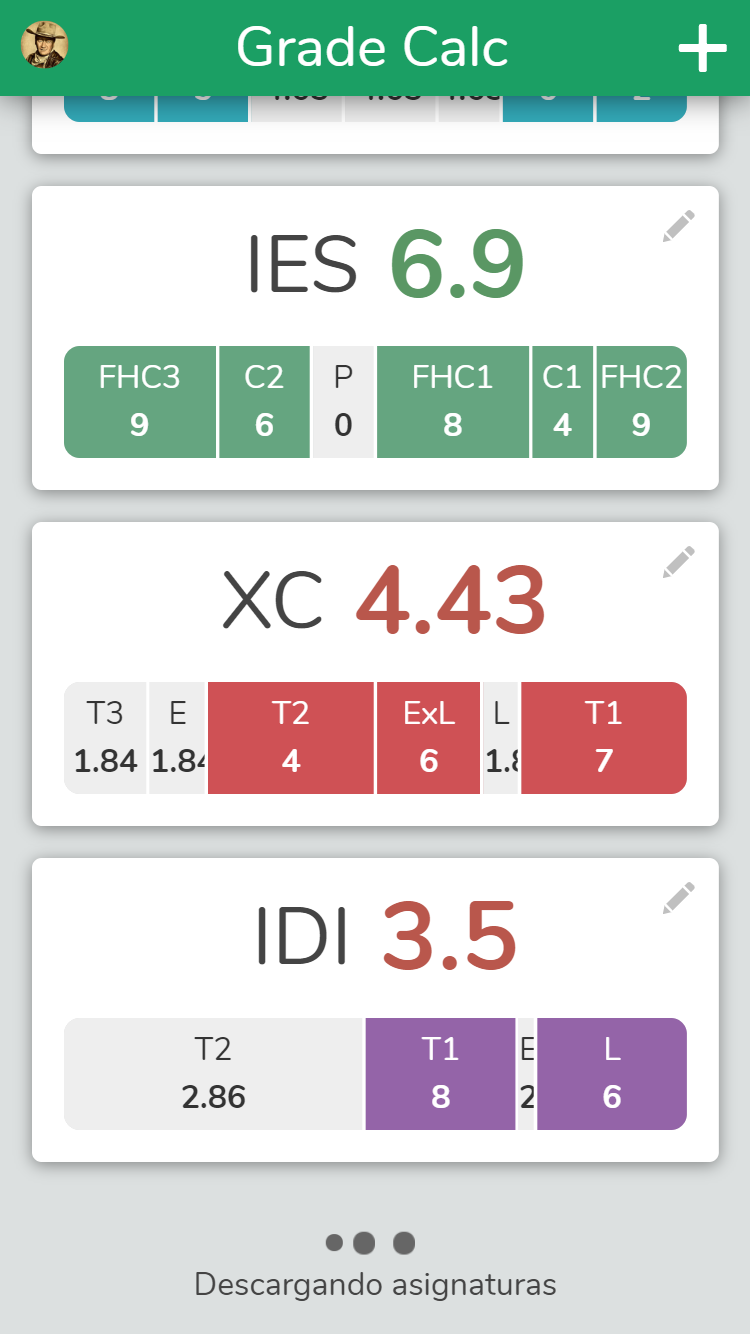
\includegraphics[width=\textwidth]{media/screenshots/screenshot-loader-descargando.png}
        \caption{Downloading}
    \end{subfigure}
    \caption{Background tasks spinner}
    \label{fig:spinner}
\end{figure}
\vfill

\clearpage\newpage
\subsubsection{Blocking spinner}

It's a loading screen that doesn't allow any interaction with the app until it finishes loading. It's annoying, so it's only used when it's unavoidable. If it exceeds the maximum expected loading time, a message appears to let the user know that something went wrong.

% , like when creating a subject (Fig. \ref{fig:create})

\vfill
\begin{figure}[ht!]
    \begin{subfigure}[b]{0.757\textwidth-0.1cm}
        \centering
        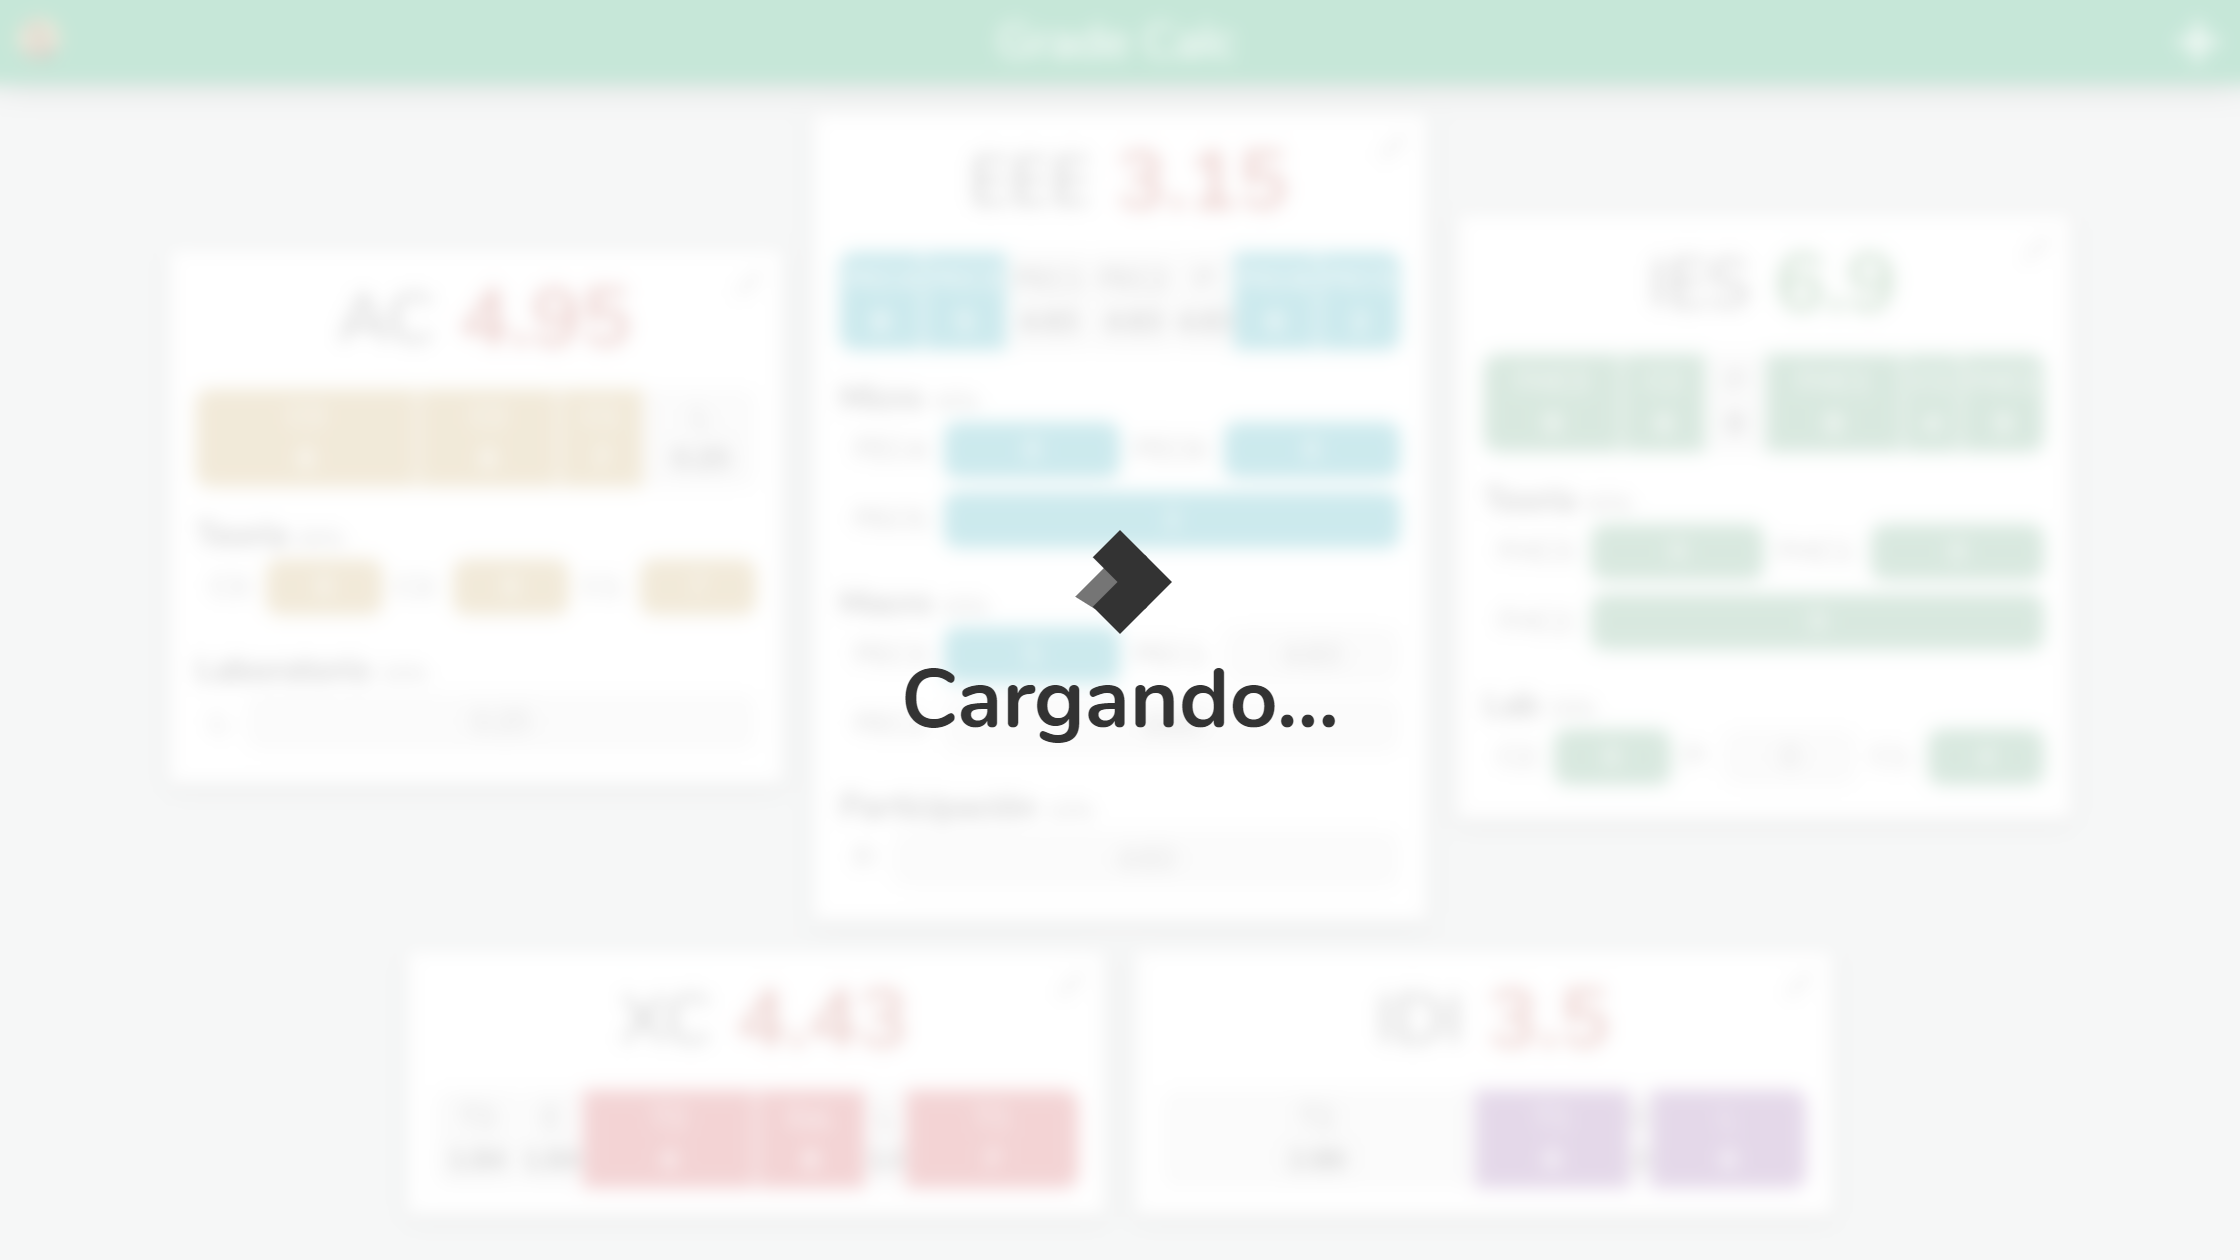
\includegraphics[frame,width=\textwidth]{media/screenshots/screenshot-froozen-pc.png}
        \caption{Desktop version}
    \end{subfigure}
    \hfill
    \begin{subfigure}[b]{0.243\textwidth-0.1cm}
        \centering
        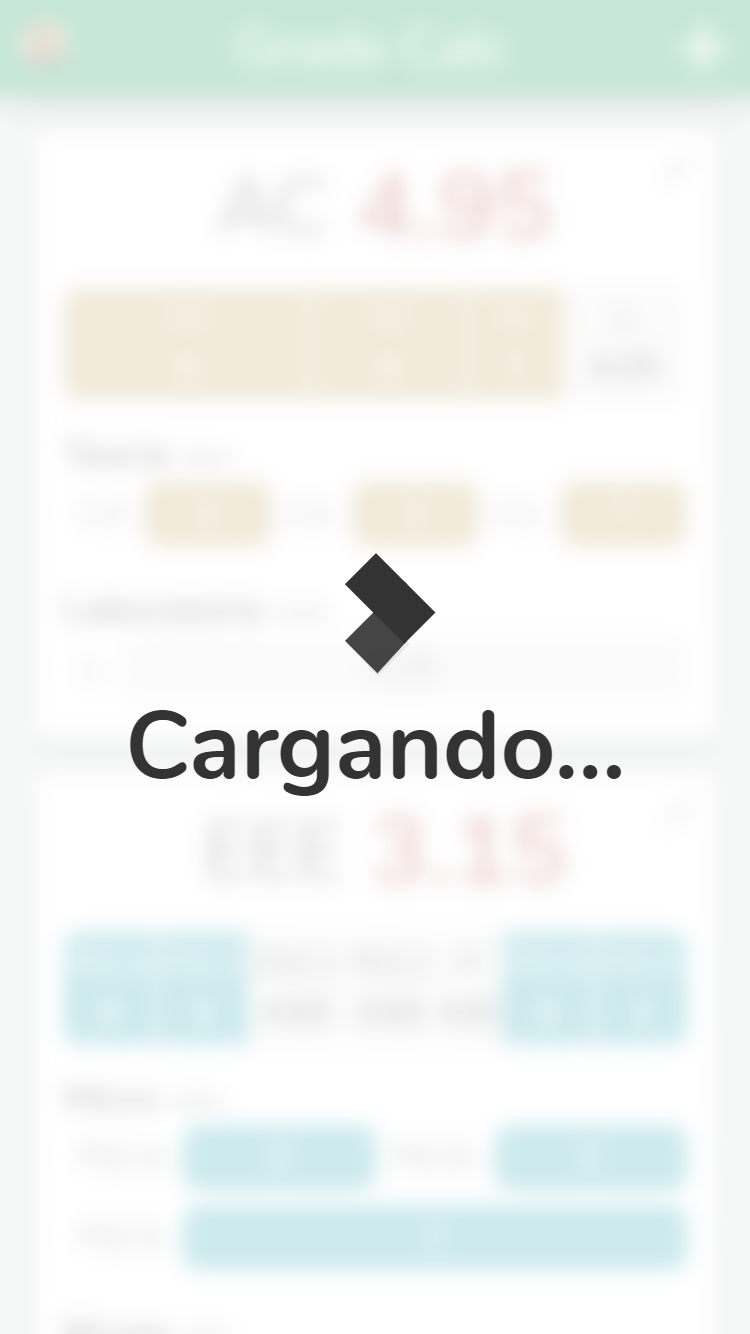
\includegraphics[frame,width=\textwidth]{media/screenshots/screenshot-froozen.png}
        \caption{Mobile version}
    \end{subfigure}
    \caption{Blocking spinner}
    \label{fig:freeze}
\end{figure}

\vfill

\begin{figure}[ht!]
    \begin{subfigure}[b]{0.757\textwidth-0.1cm}
        \centering
        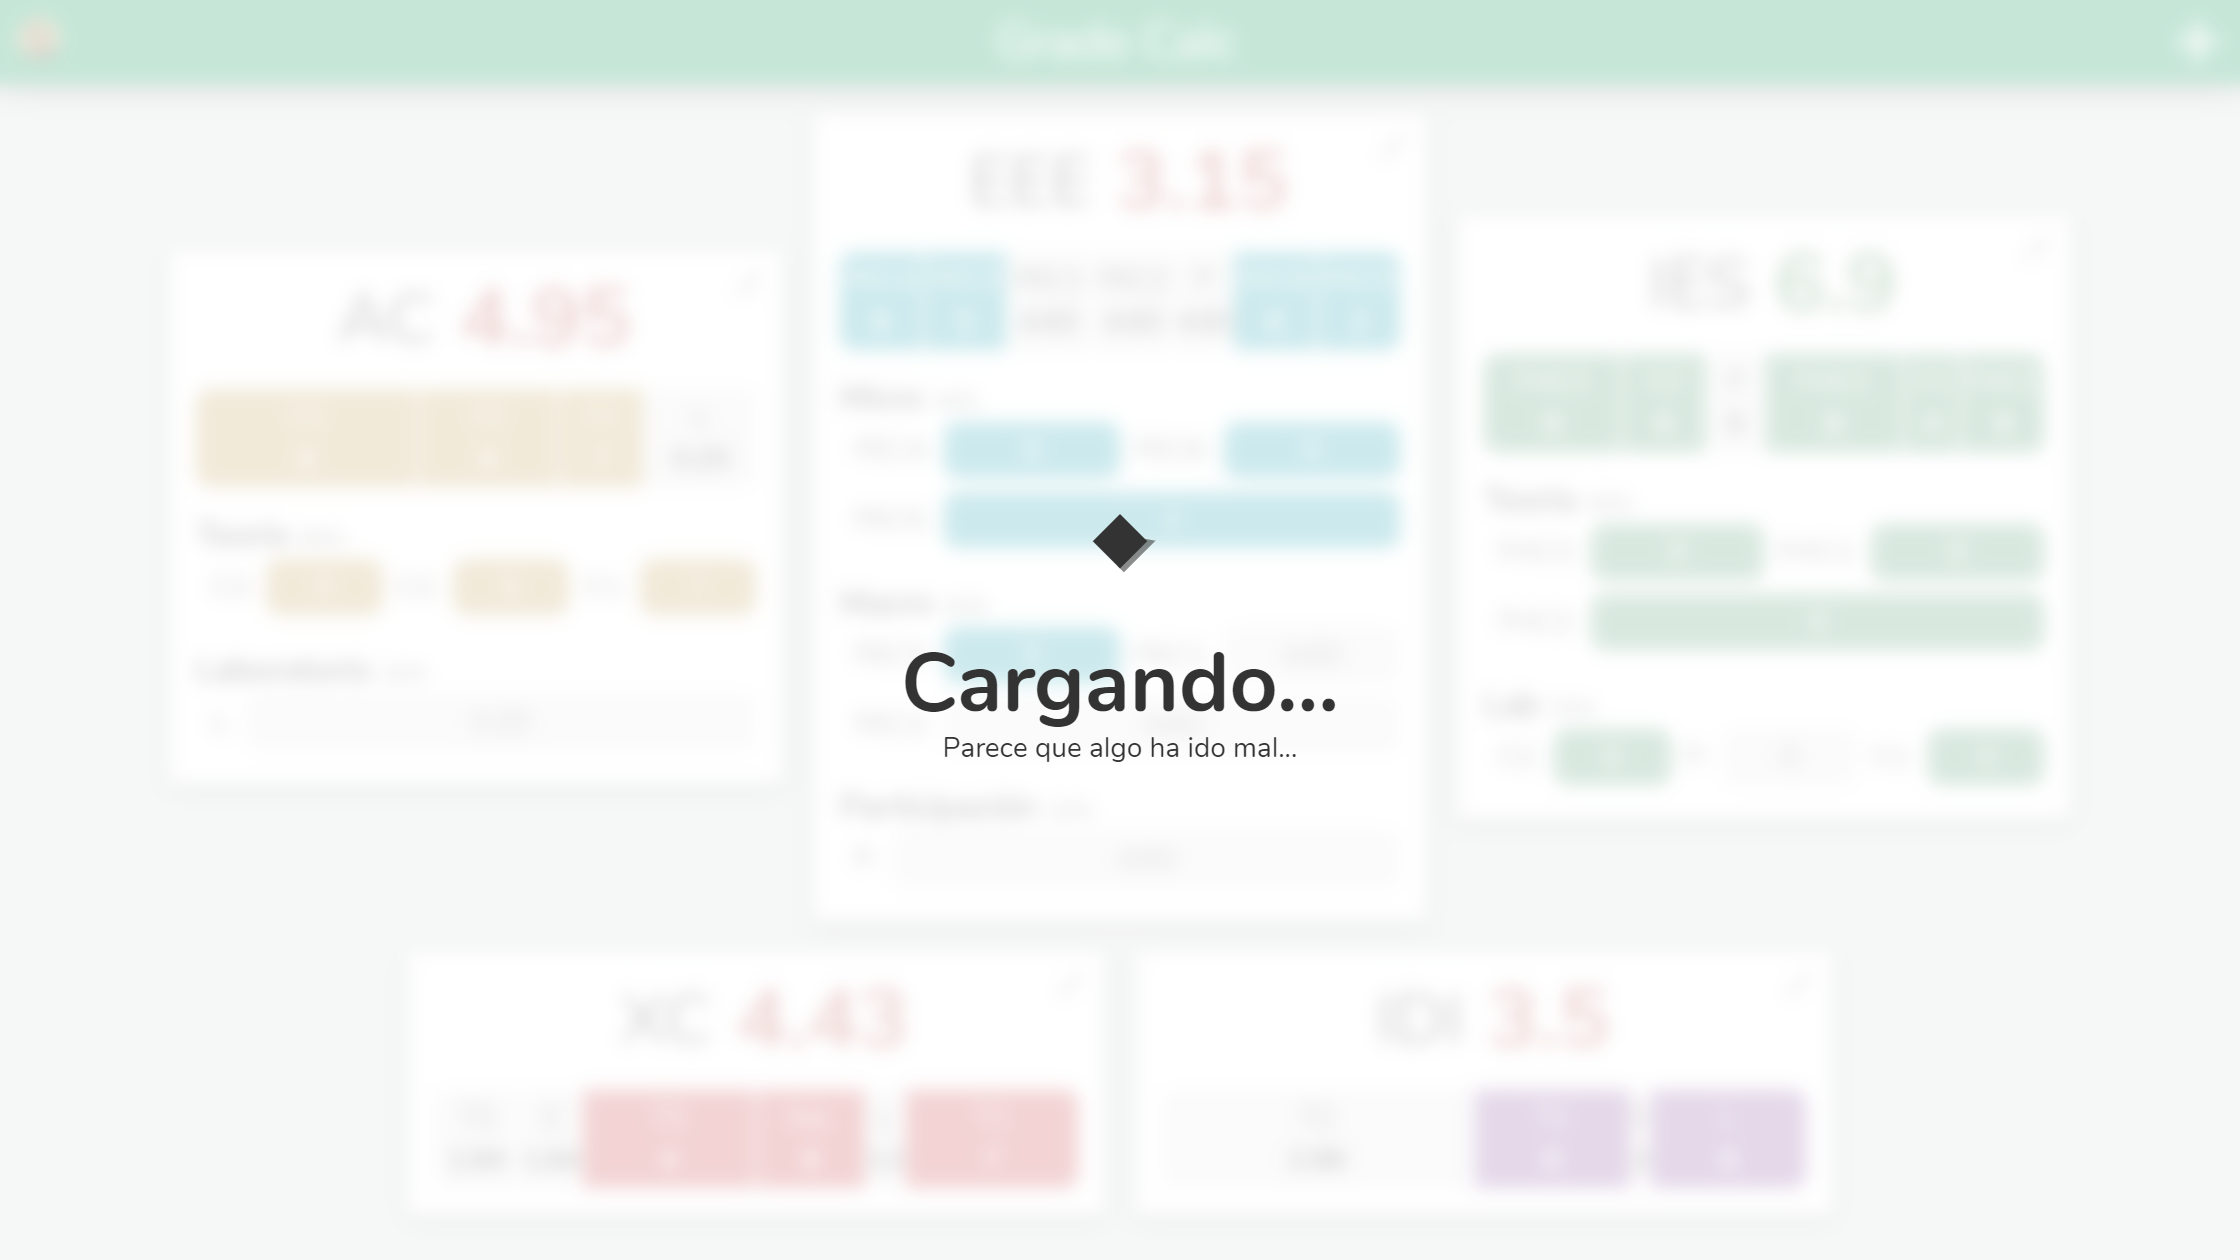
\includegraphics[frame,width=\textwidth]{media/screenshots/screenshot-froozen-long-pc.png}
        \caption{Desktop version}
    \end{subfigure}
    \hfill
    \begin{subfigure}[b]{0.243\textwidth-0.1cm}
        \centering
        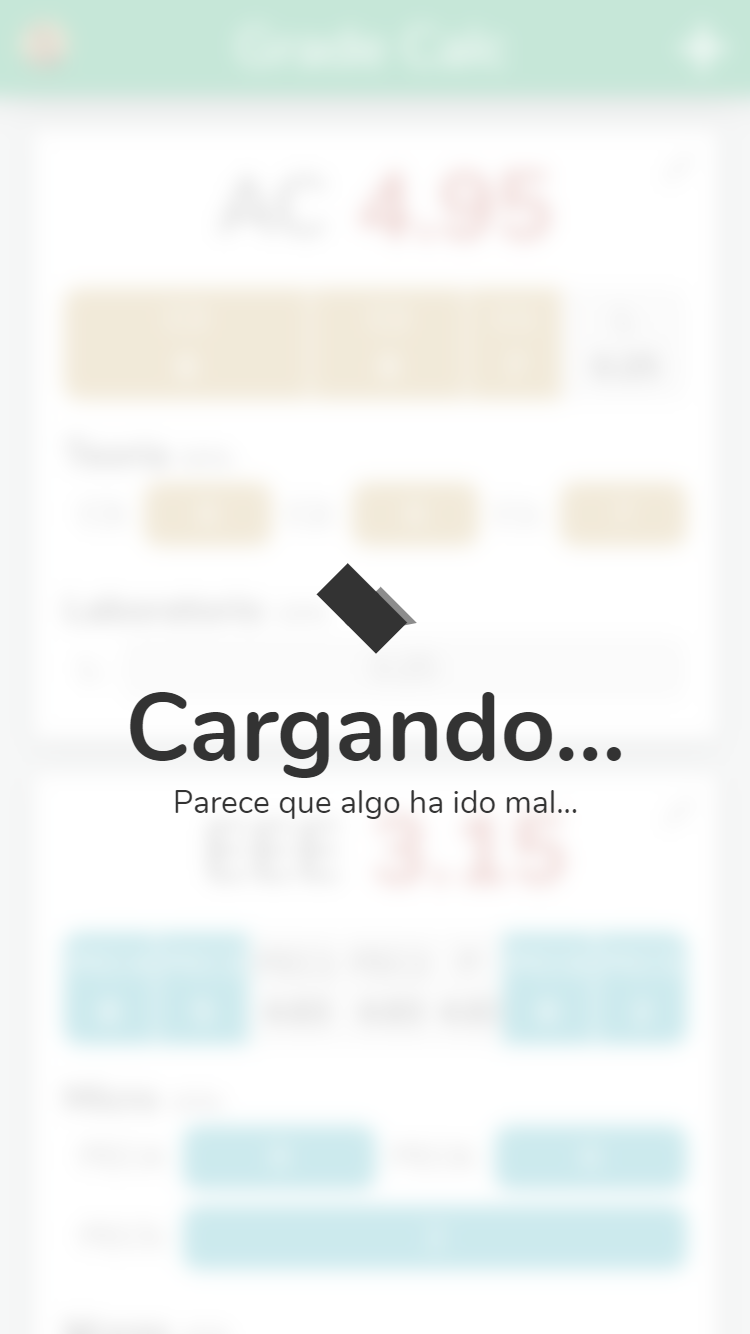
\includegraphics[frame,width=\textwidth]{media/screenshots/screenshot-froozen-long.png}
        \caption{Mobile version}
    \end{subfigure}
    \caption{Blocking spinner taking too much time}
    \label{fig:lading-long}
\end{figure}
\vfill

\clearpage\newpage
\subsubsection{Notifications}

These are notifications in a snackbar\cite{snackbar} style that appears at the bottom of the screen for a short time, the default is 8 seconds. They consist of a text and an optional action. 

In the examples below (Fig. \ref{fig:notifications}) we can see the four most common notifications:
\begin{enumerate}[label=\textbf{(\alph*)},itemsep=0mm]
    \item \textbf{Log-in}: It appears when the app is opened and the user is not logged-in. Its action is the same as the \inlineicon{button-login.png} button.
    \item \textbf{Undo}: It appears when a subject card is deleted. Its action restores the subject. It lets undo a destructive action to prevent unwanted losses of data.
    \item \textbf{Install}: It appears when the app is opened, after the log-in notification, if the app meets the PWA installation criteria\cite{pwa-install-criteria}. Its action shows the install prompt, more details in section \ref{sec:install}.
    \item \textbf{Error}: It appears when there's an error, for example, an invalid value in the edit subject screen (Fig. \ref{fig:edit}).
\end{enumerate}

\vfill
\begin{figure}[ht!]
    \begin{subfigure}[b]{0.25\textwidth-0.1cm}
        \centering
        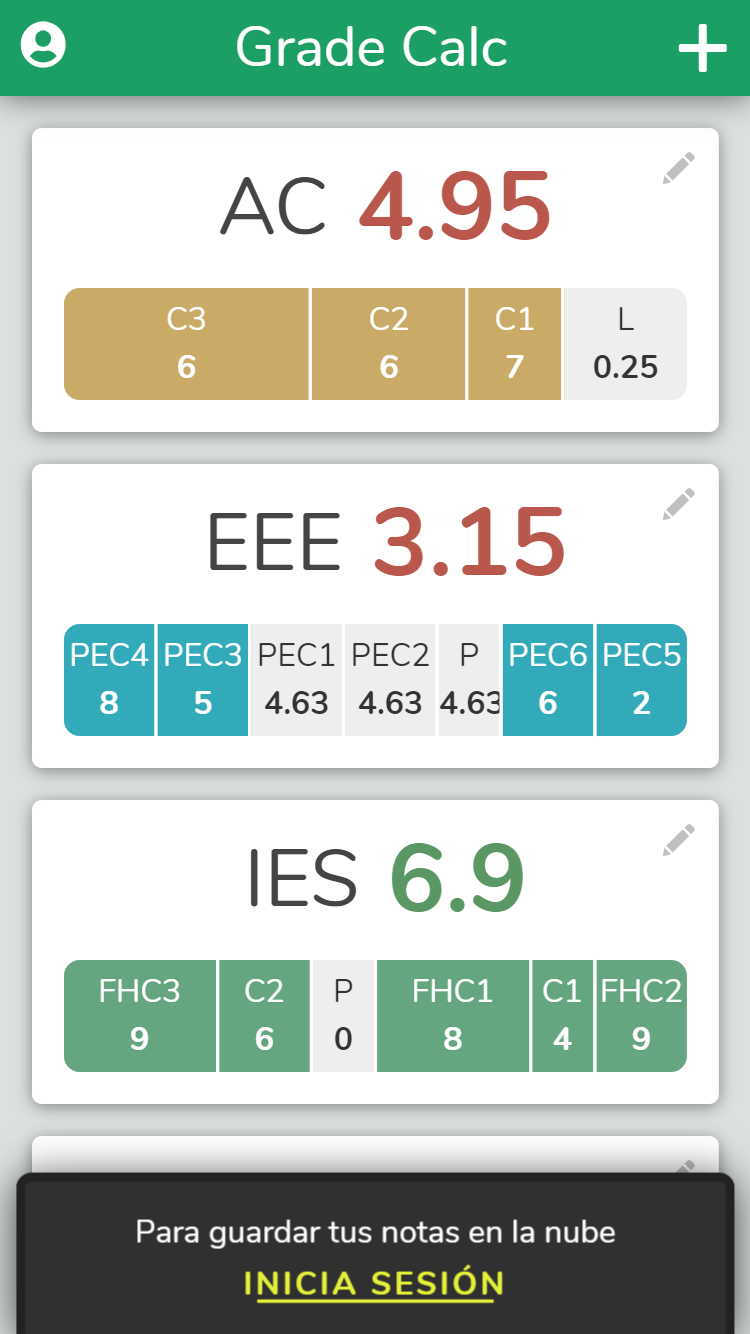
\includegraphics[width=\textwidth]{media/screenshots/screenshot-notification-login.png}
        \caption{Log-in}
    \end{subfigure}
    \hfill
    \begin{subfigure}[b]{0.25\textwidth-0.1cm}
        \centering
        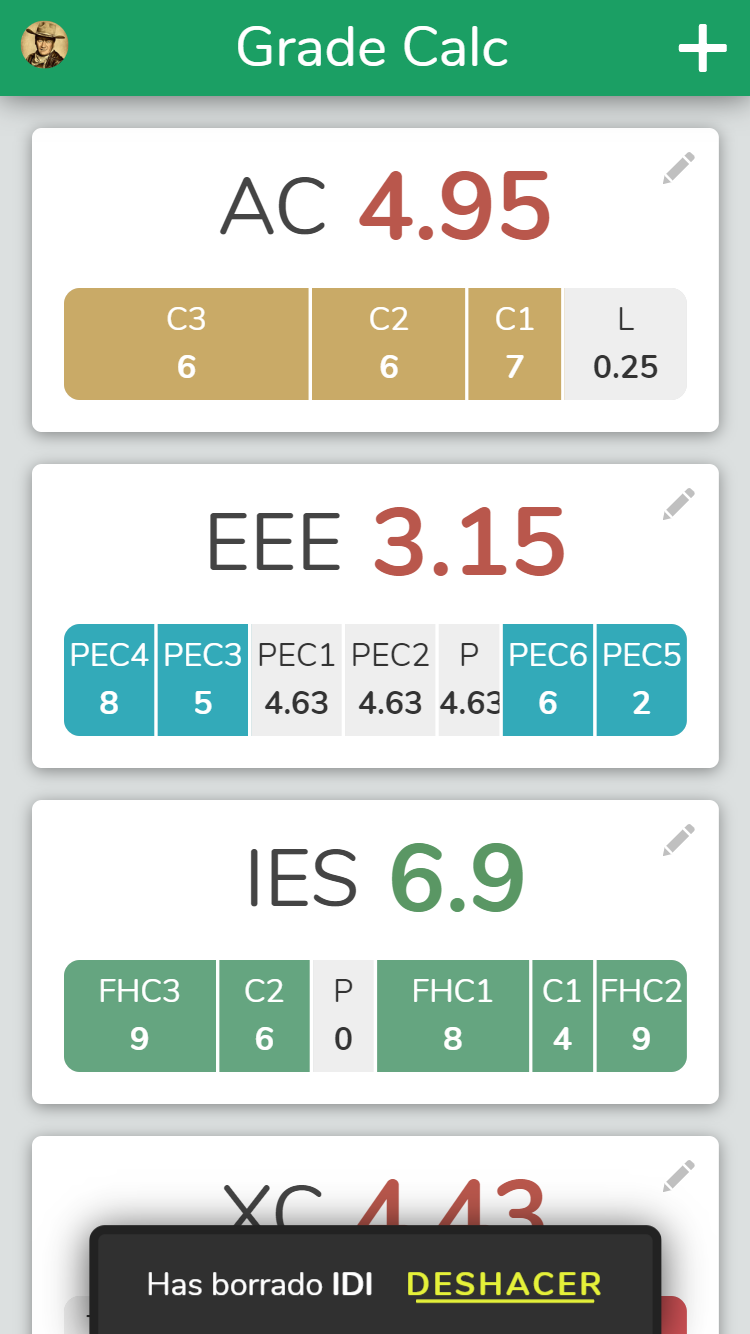
\includegraphics[width=\textwidth]{media/screenshots/screenshot-notification-undo.png}
        \caption{Undo}
    \end{subfigure}
    \hfill
    \begin{subfigure}[b]{0.25\textwidth-0.1cm}
        \centering
        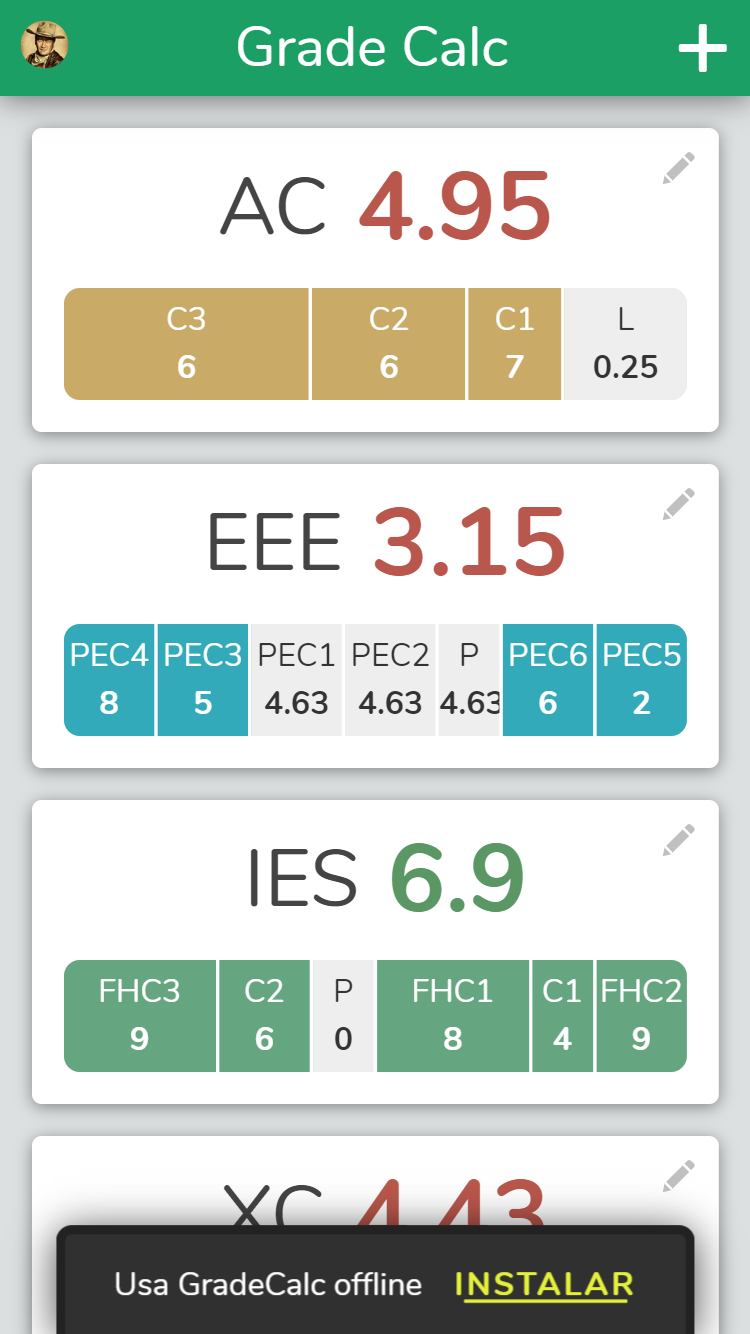
\includegraphics[width=\textwidth]{media/screenshots/screenshot-notification-install.png}
        \caption{Install}
    \end{subfigure}
    \hfill
    \begin{subfigure}[b]{0.25\textwidth-0.1cm}
        \centering
        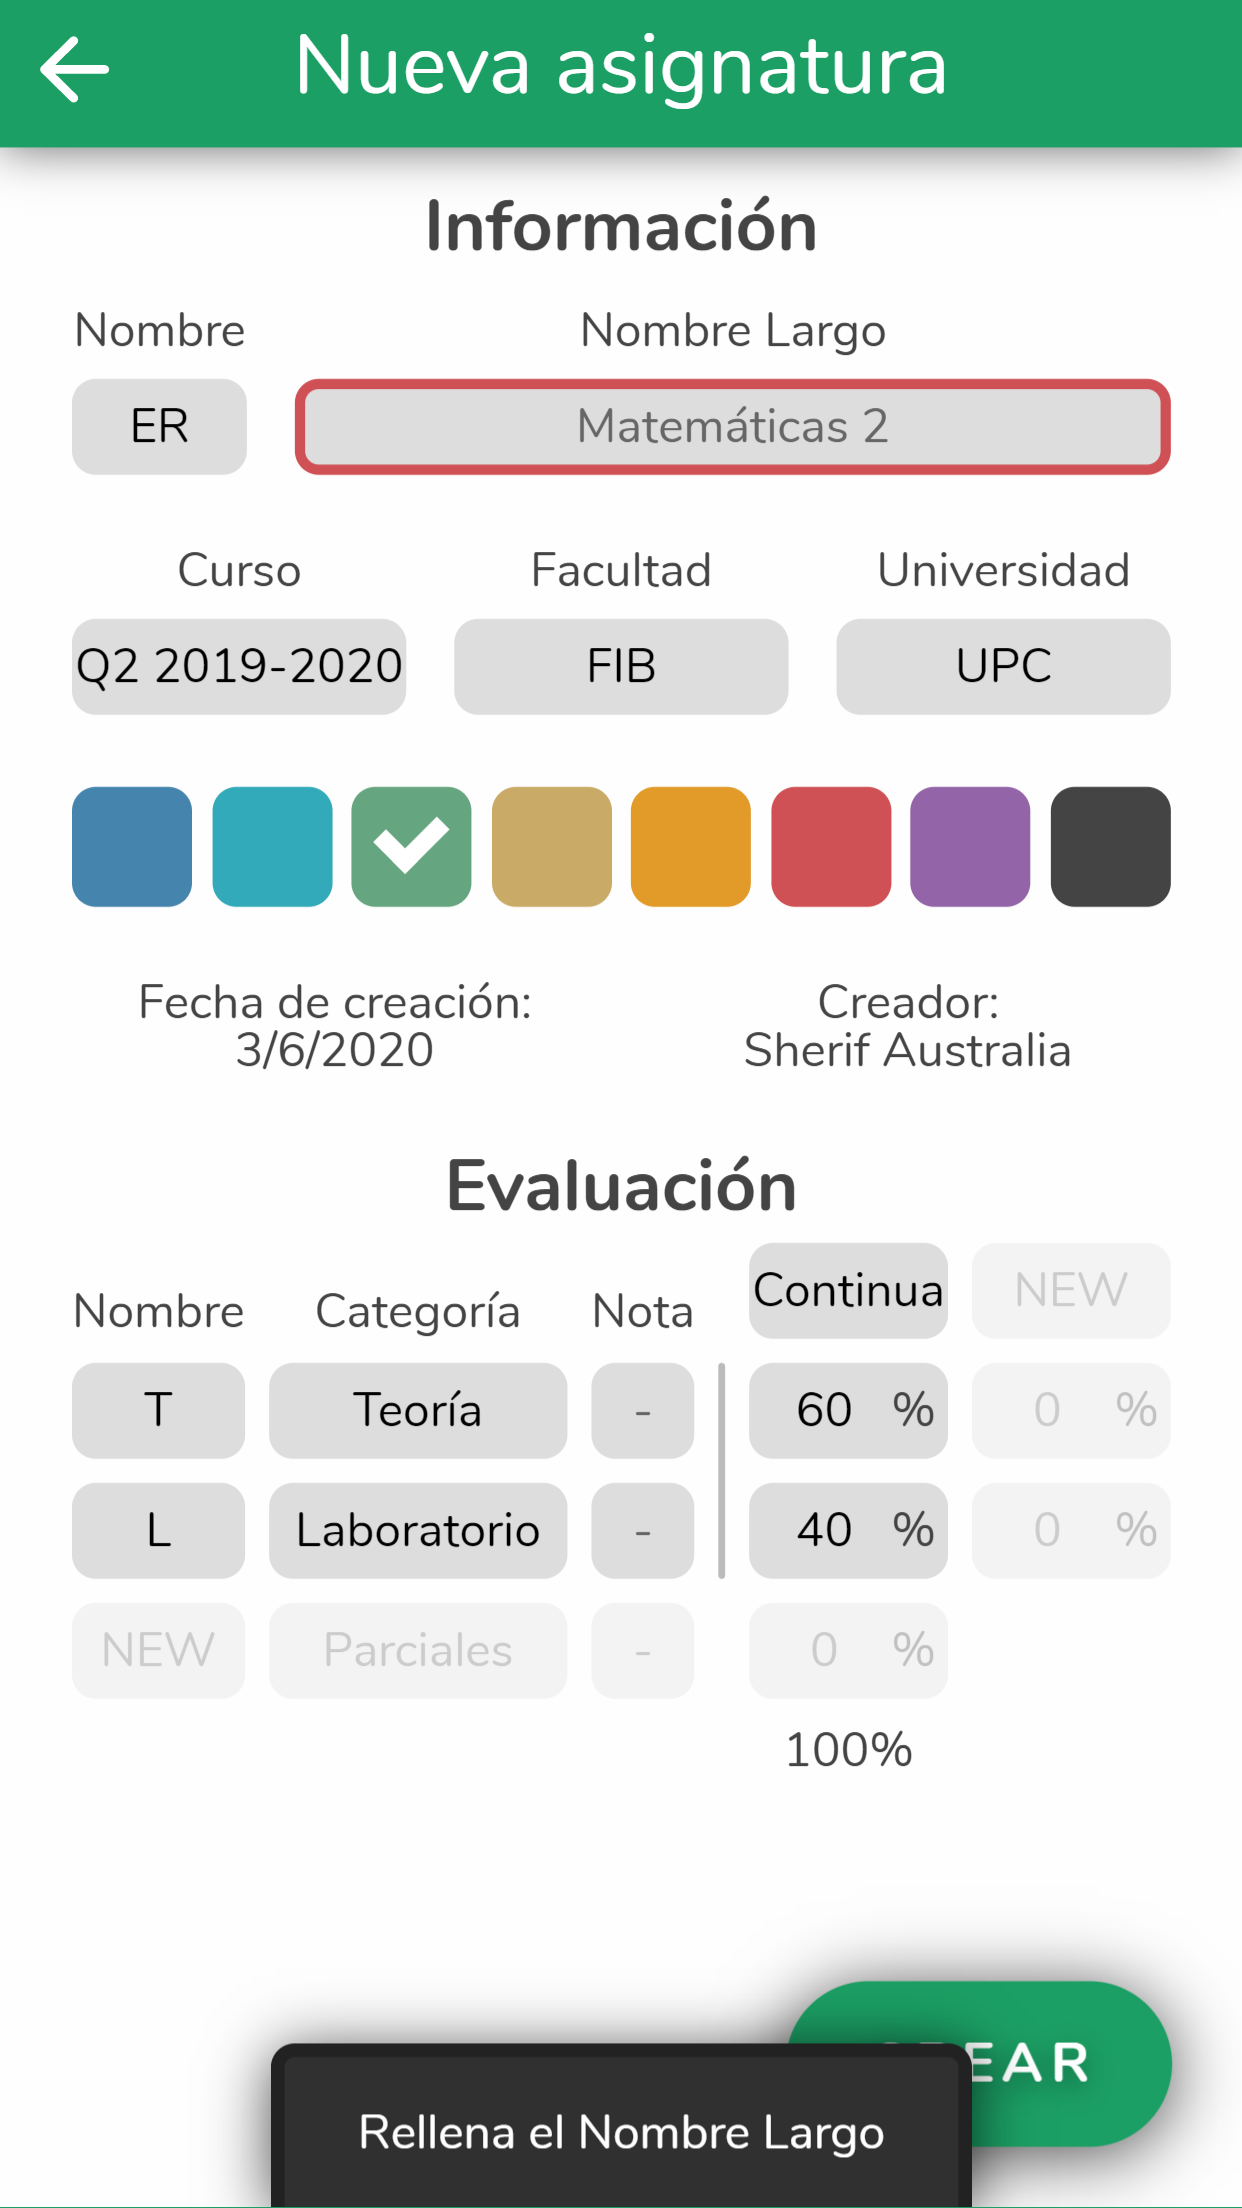
\includegraphics[width=\textwidth]{media/screenshots/screenshot-notification-error.png}
        \caption{Error}
    \end{subfigure}
    \caption{Notifications}
    \label{fig:notifications}
\end{figure}
\vfill

\clearpage\newpage
\subsubsection{Install prompt}
\label{sec:install}

This is the prompt that the operating system shows to confirm the installation of the app (Fig. \ref{fig:install-prompt}). It shows up in these two scenarios:

\begin{itemize}
    \item When the user clicks the action of the install notification (Fig. \ref{fig:install-banner}).
    \item When the user clicks the \textit{Install} button from the browser's UI, its location and label may be different across browsers.
\end{itemize}

Once the app is installed it's icon appears in the device's home screen and the app will open in standalone mode\footnote{The browser UI elements like the address bar and navigation are hidden.}. The icon has 3 versions (Fig. \ref{fig:gradecalc-app-icon}) to comply to each platform design guidelines. 

The app can be installed in: \textit{Android}, \textit{iOS}, \textit{Windows}, \textit{macOS} and \textit{Linux}. The example below (Fig. \ref{fig:install}) is how to installation process looks in Android 10.


\vfill
\begin{figure}[ht!]
    \begin{subfigure}[b]{0.25\textwidth-0.1cm}
        \centering
        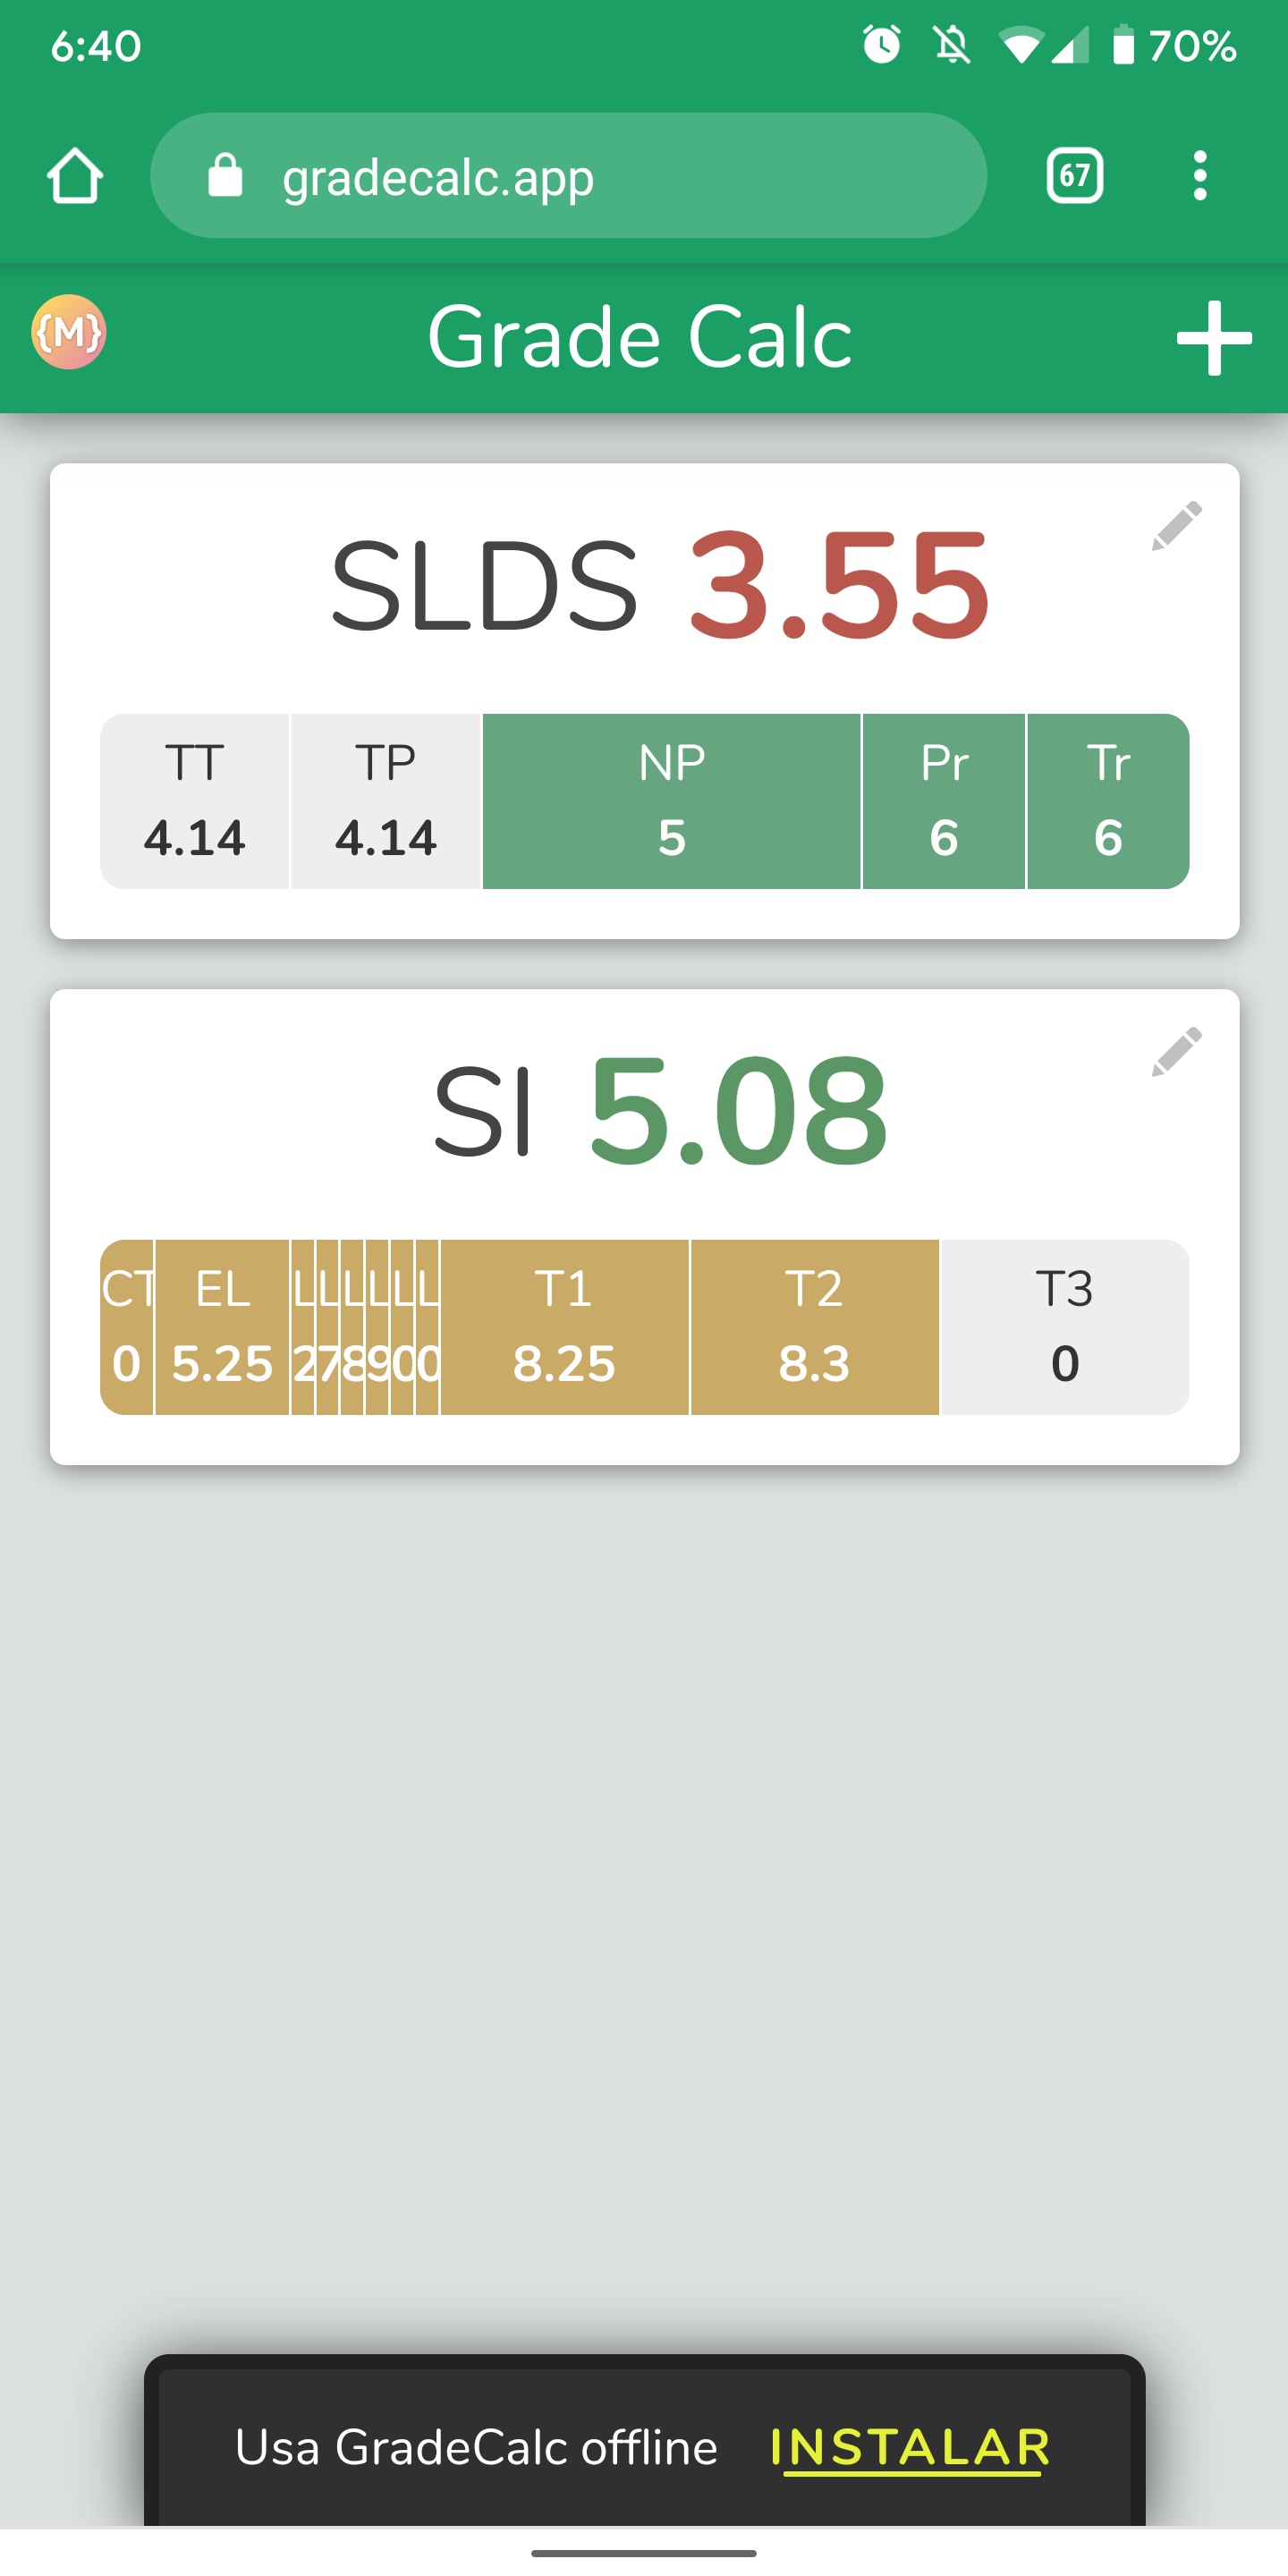
\includegraphics[width=\textwidth]{media/screenshots/screenshot-install-banner.png}
        \caption{Banner}
        \label{fig:install-banner}
    \end{subfigure}
    \hfill
    \begin{subfigure}[b]{0.25\textwidth-0.1cm}
        \centering
        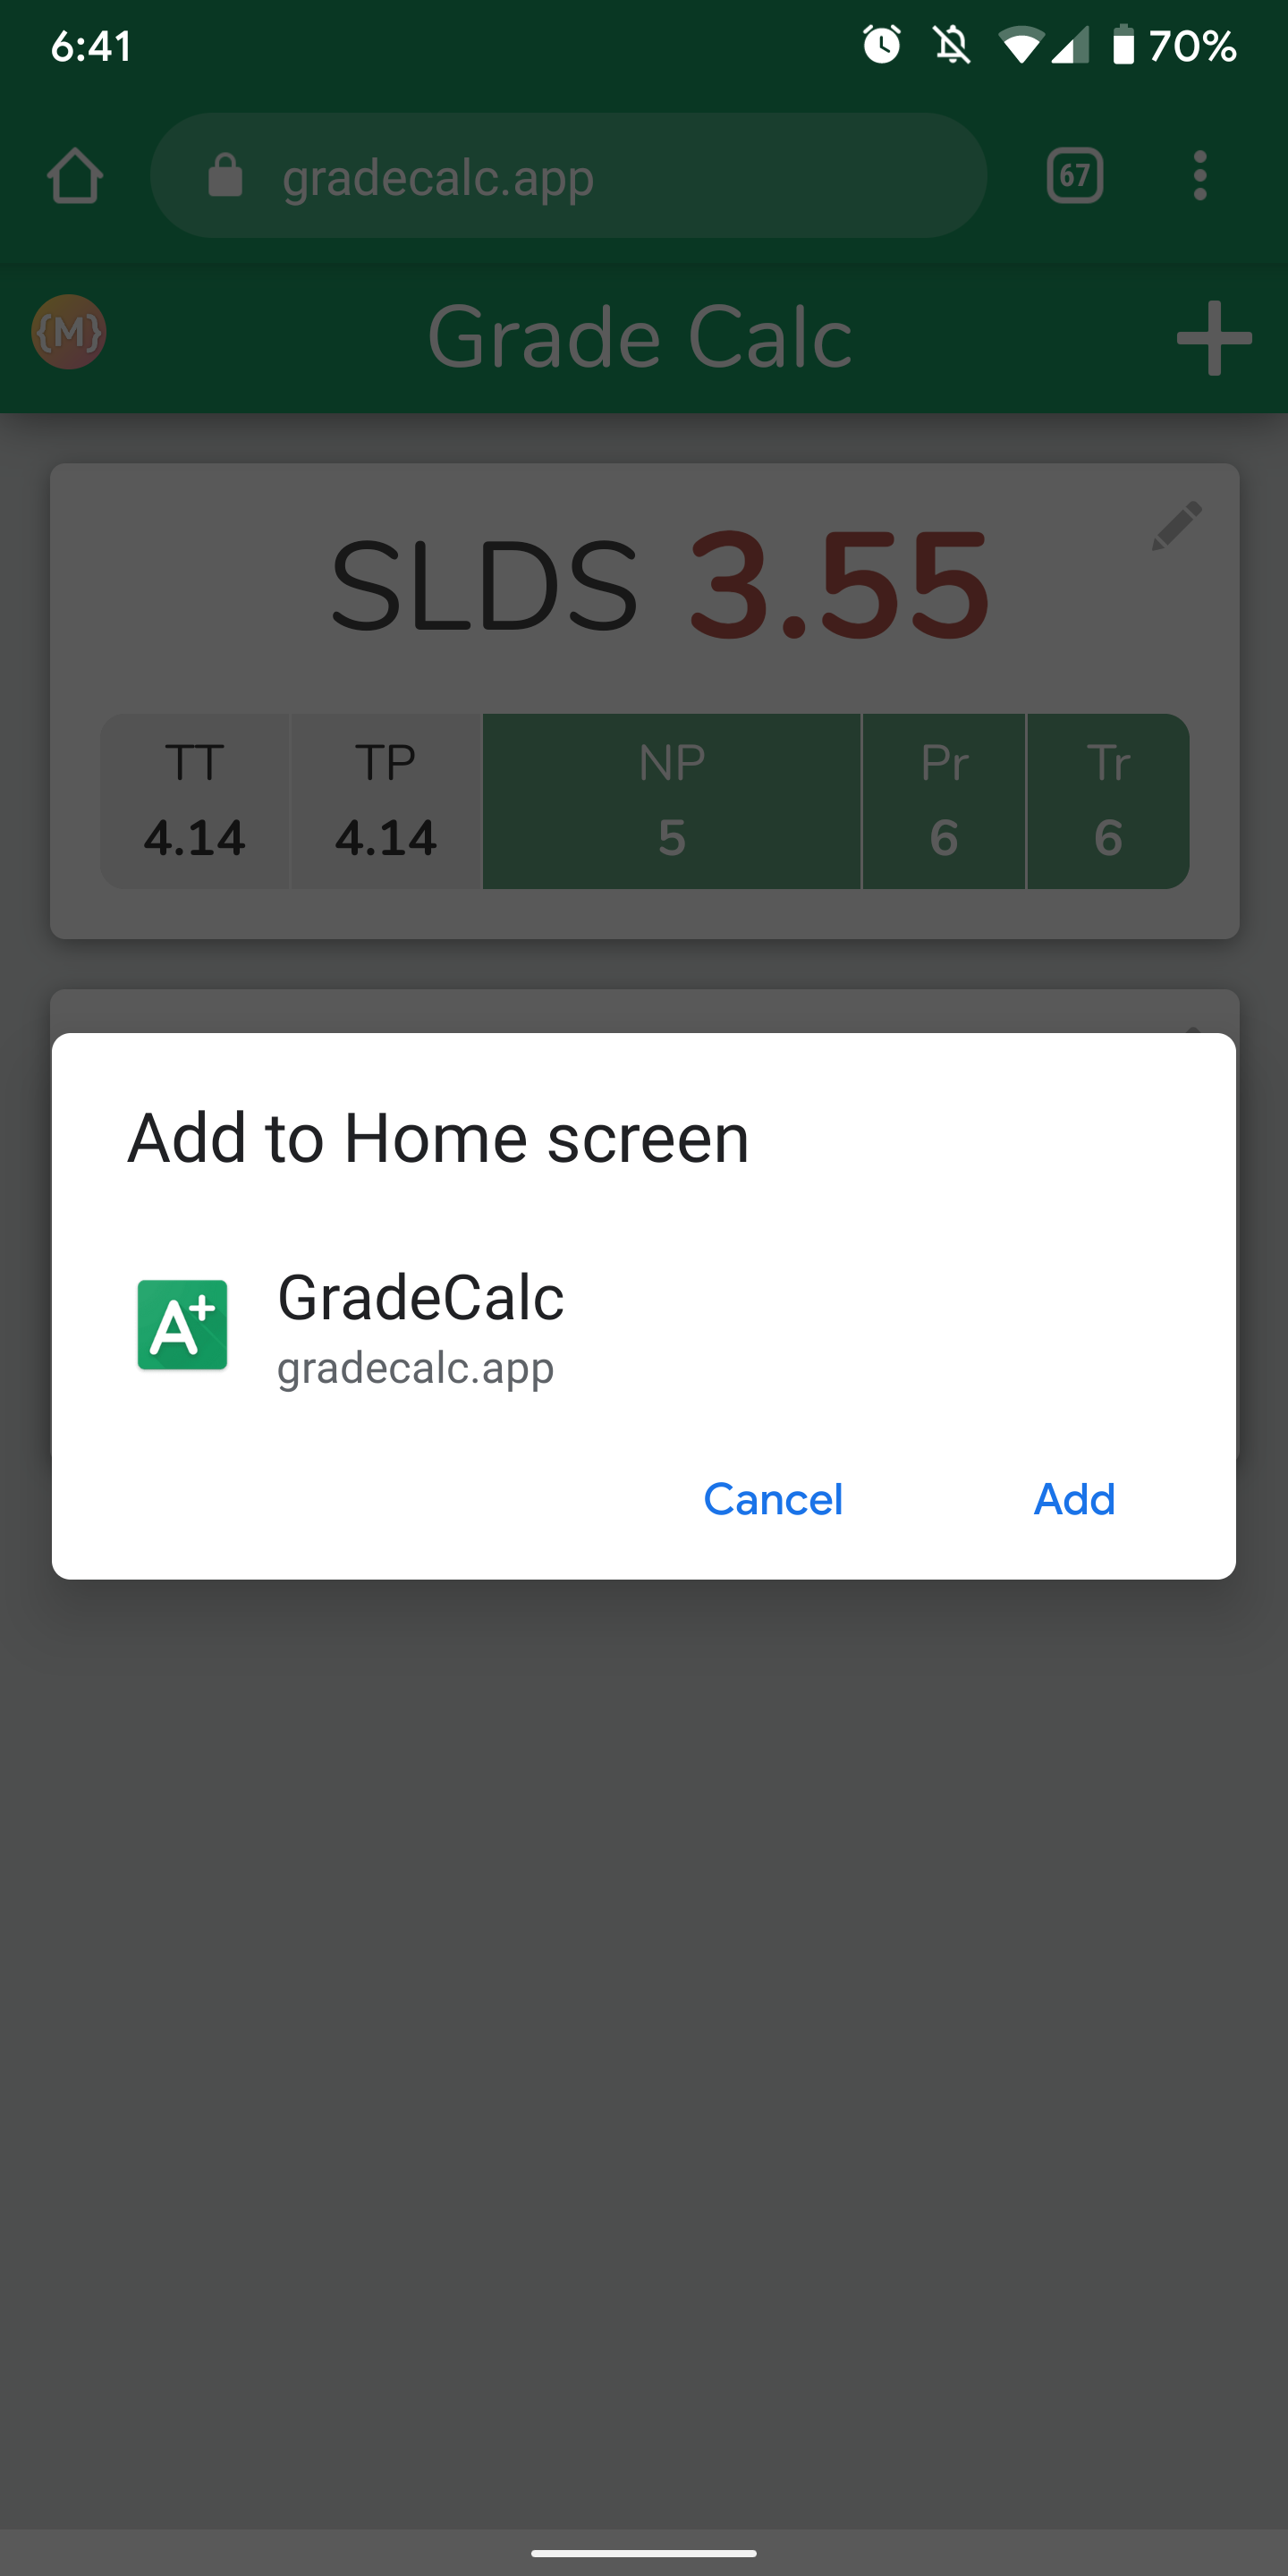
\includegraphics[width=\textwidth]{media/screenshots/screenshot-install-popup.png}
        \caption{Confirmation}
        \label{fig:install-prompt}
    \end{subfigure}
    \hfill
    \begin{subfigure}[b]{0.25\textwidth-0.1cm}
        \centering
        
\includegraphics[width=\textwidth]{media/screenshots/screenshot-install-homescreen.png}
        \caption{Icon}
    \end{subfigure}
    \hfill
    \begin{subfigure}[b]{0.25\textwidth-0.1cm}
        \centering
        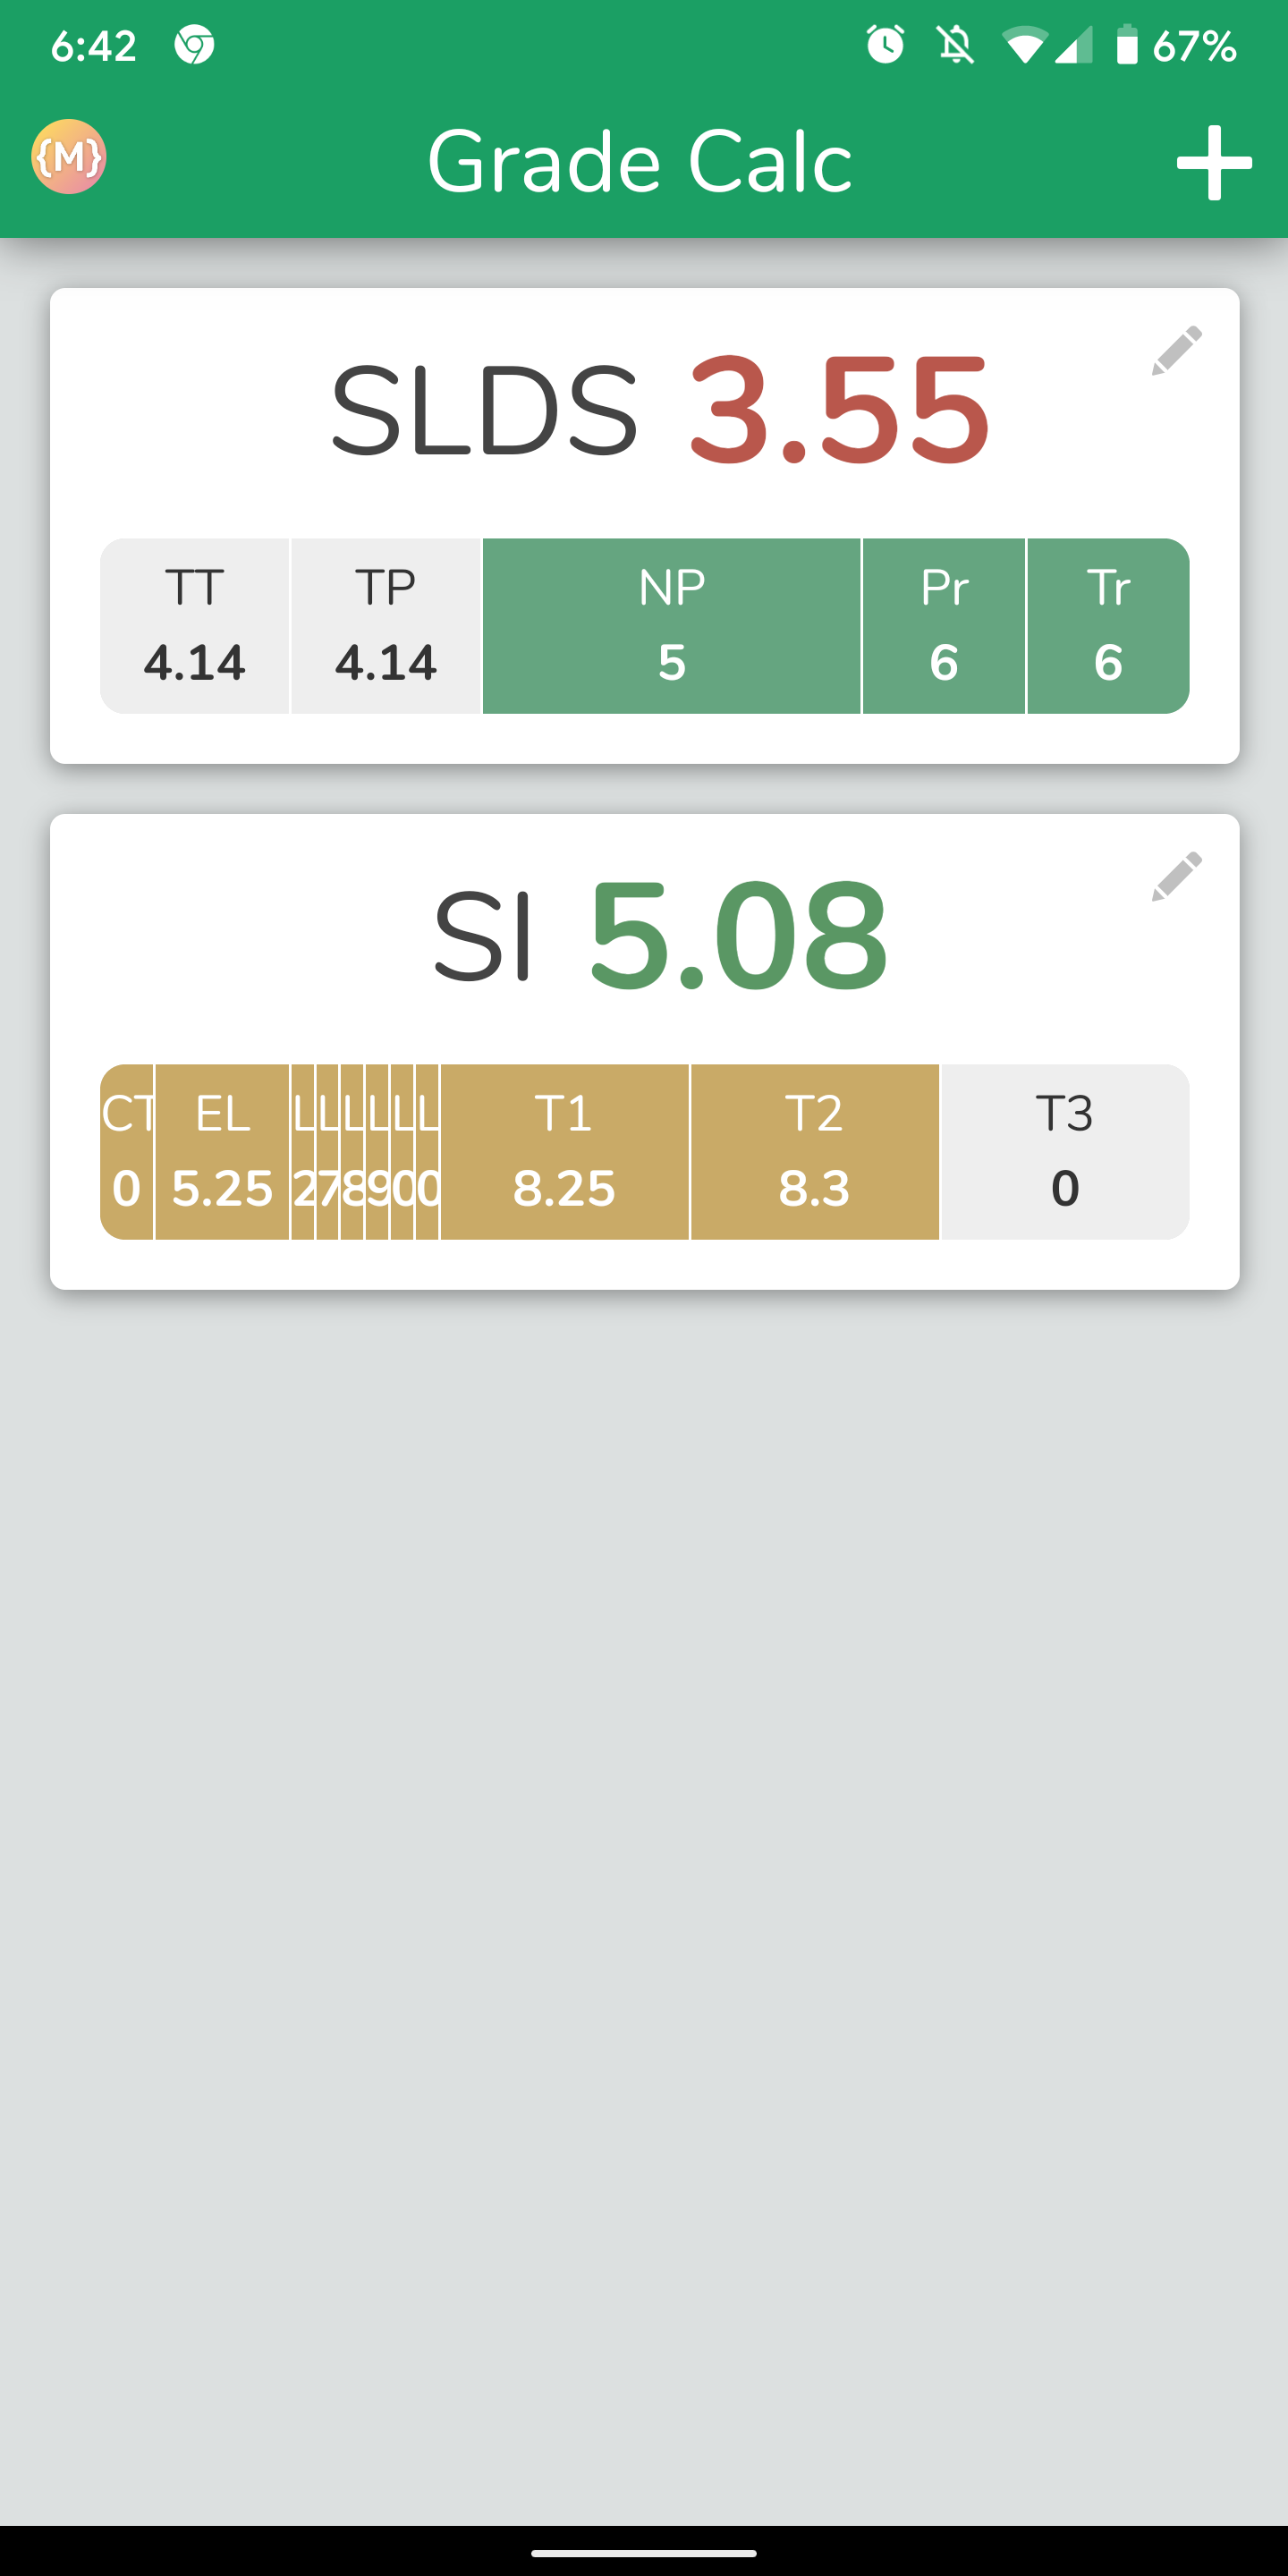
\includegraphics[width=\textwidth]{media/screenshots/screenshot-install-standalone.png}
        \caption{Installed app}
    \end{subfigure}
    \caption{Installation process}
    \label{fig:install}
\end{figure}
\vfill

\clearpage\newpage
\subsubsection{Congratulations}

Finally, there's an \textbf{easter egg}\footnote{An easter egg is a hidden message, or feature in a video game, film, or other, usually electronic, medium.} in the app. To unlock it the student must pass all the subjects in the dashboard. When that happens, a gift appears (Fig. \ref{fig:gift}), with a fancy animation (Fig. \ref{fig:gift-animation}), at the bottom of the dashboard along with a congratulating text. 

% \cite{easter-egg-definition}

\vfill
\begin{figure}[ht!]
    \begin{subfigure}[b]{0.757\textwidth-0.1cm}
        \centering
        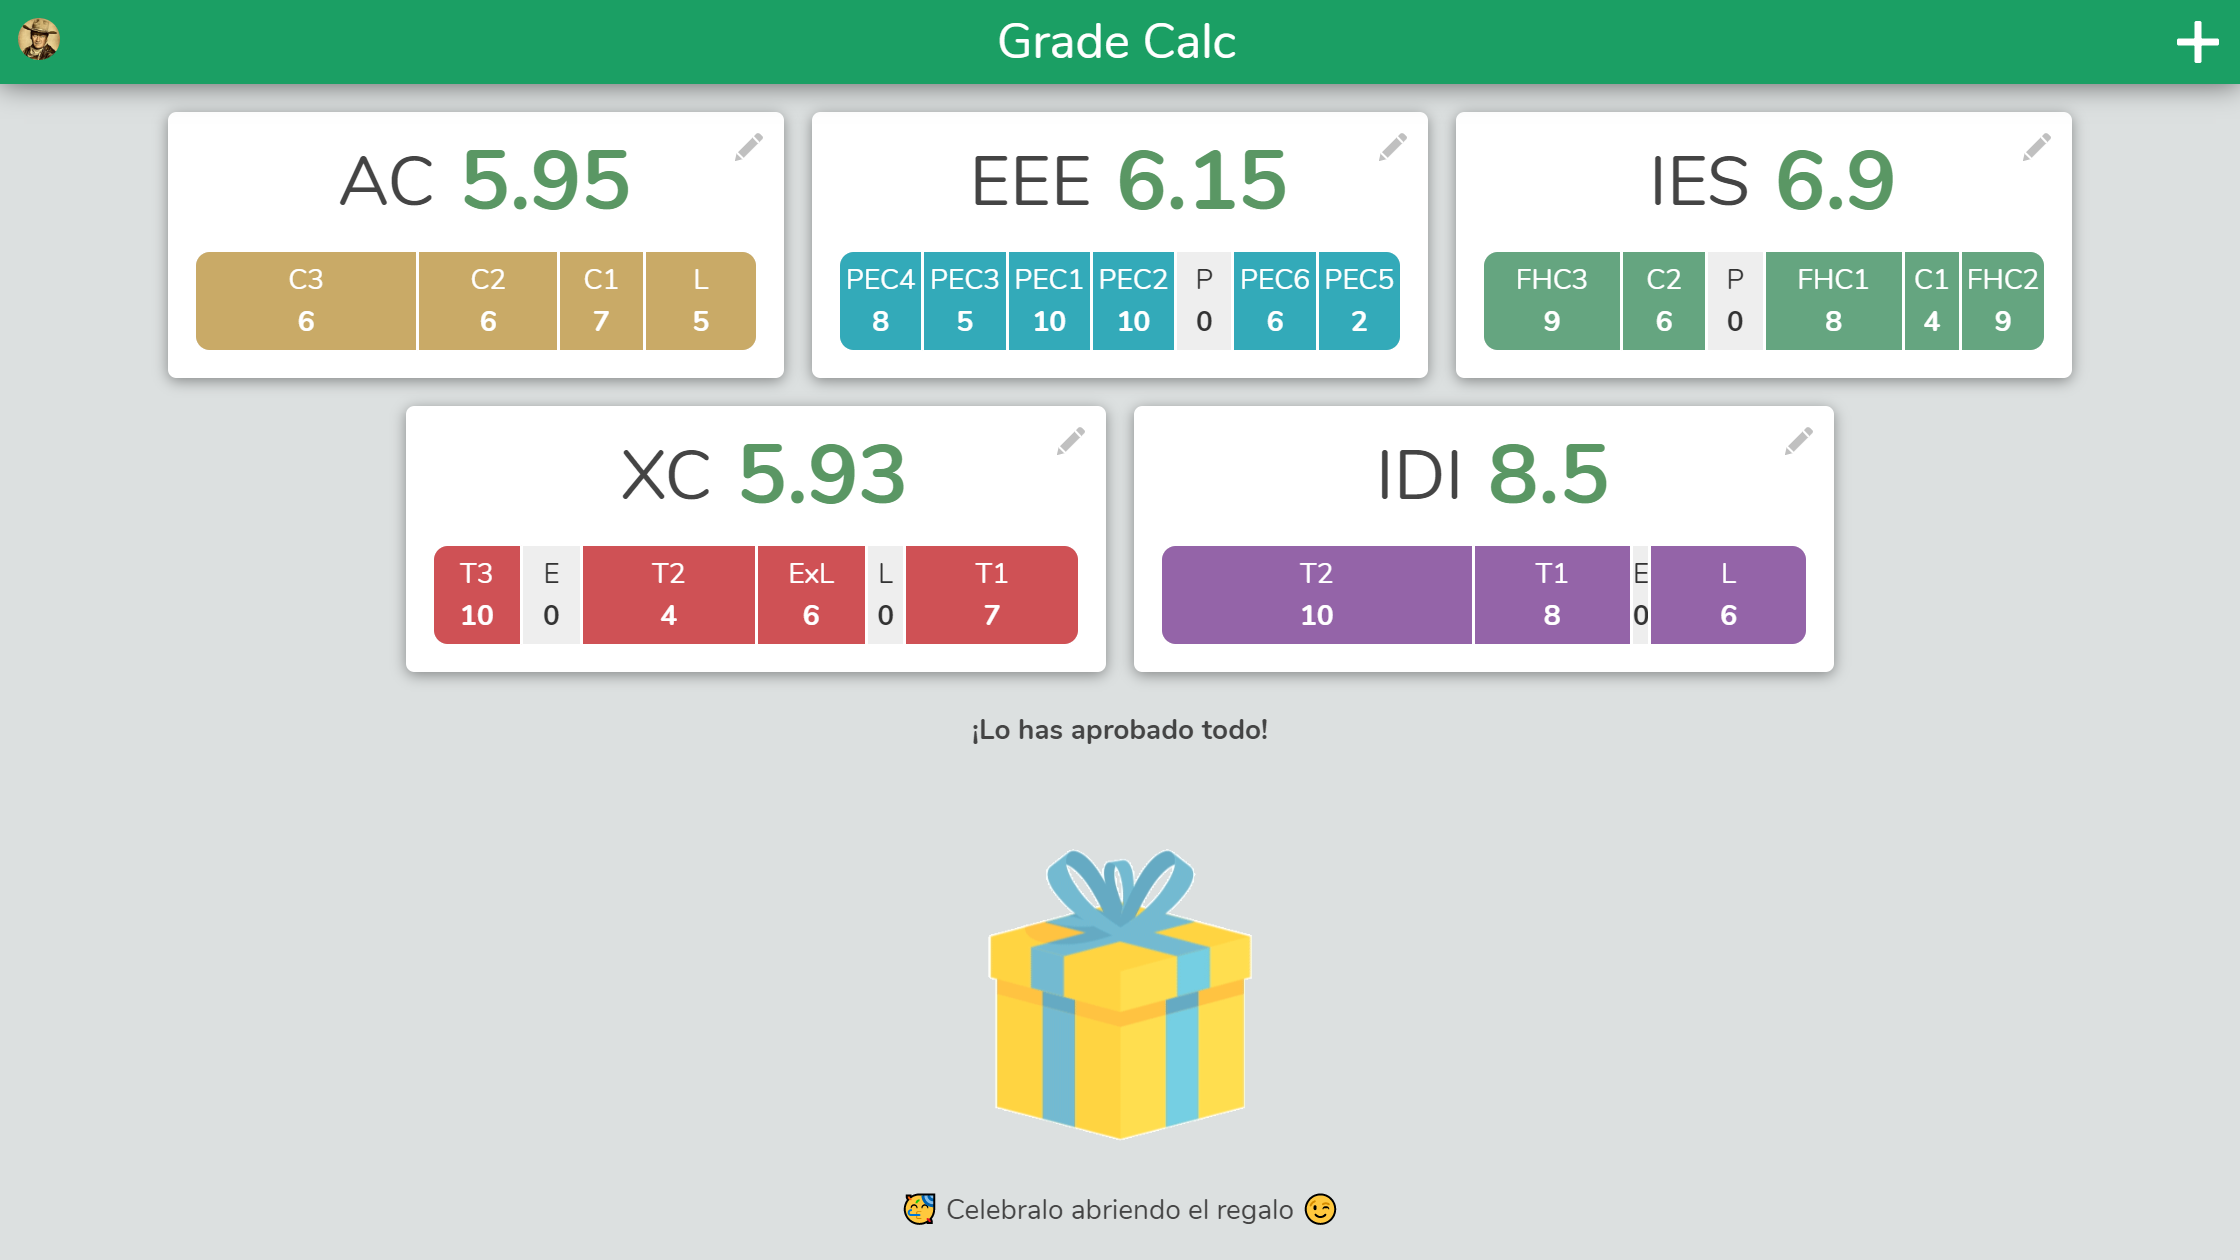
\includegraphics[width=\textwidth]{media/screenshots/screenshot-gift-pc.png}
        \caption{Desktop version}
    \end{subfigure}
    \hfill
    \begin{subfigure}[b]{0.243\textwidth-0.1cm}
        \centering
        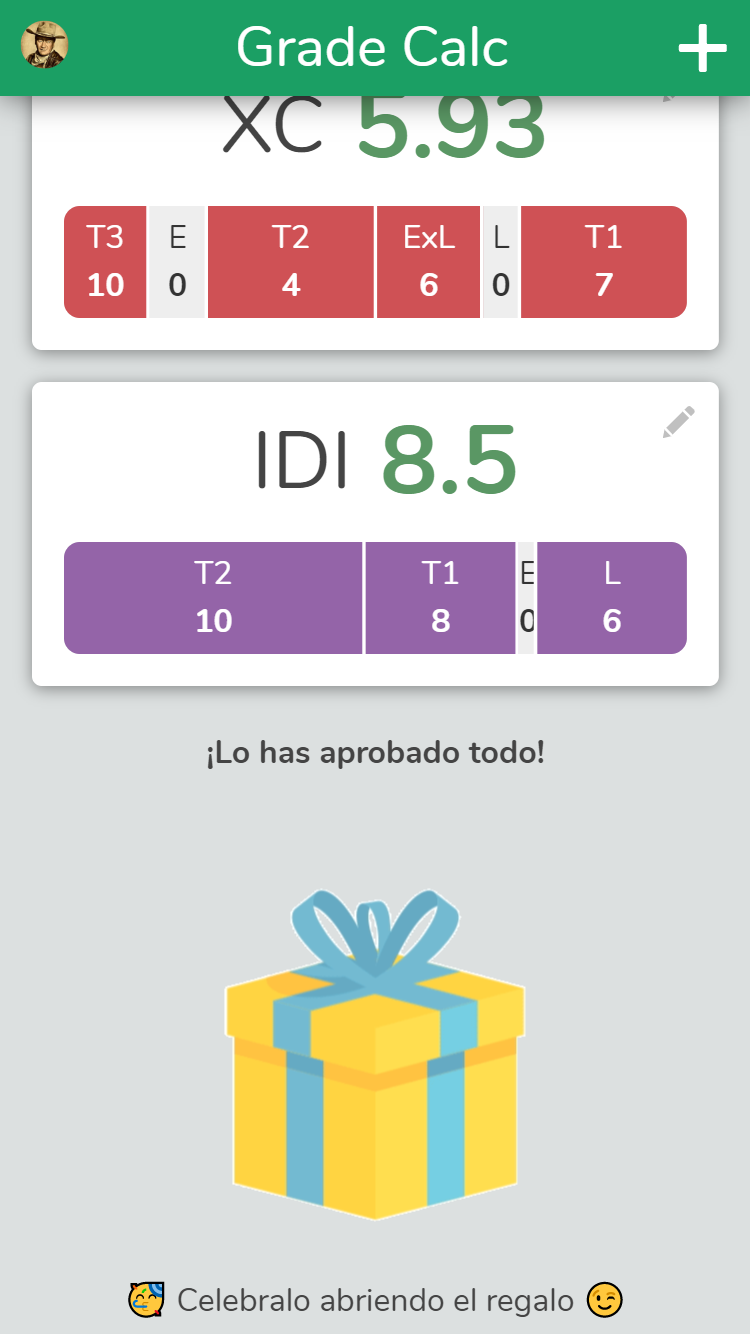
\includegraphics[width=\textwidth]{media/screenshots/screenshot-gift.png}
        \caption{Mobile version}
    \end{subfigure}
    \caption{Surprise gift}
    \label{fig:gift}
\end{figure}

\vfill

\begin{figure}[htbp!]
    \centering
    \begin{subfigure}[b]{0.23\textwidth-0.1cm}
        \centering
        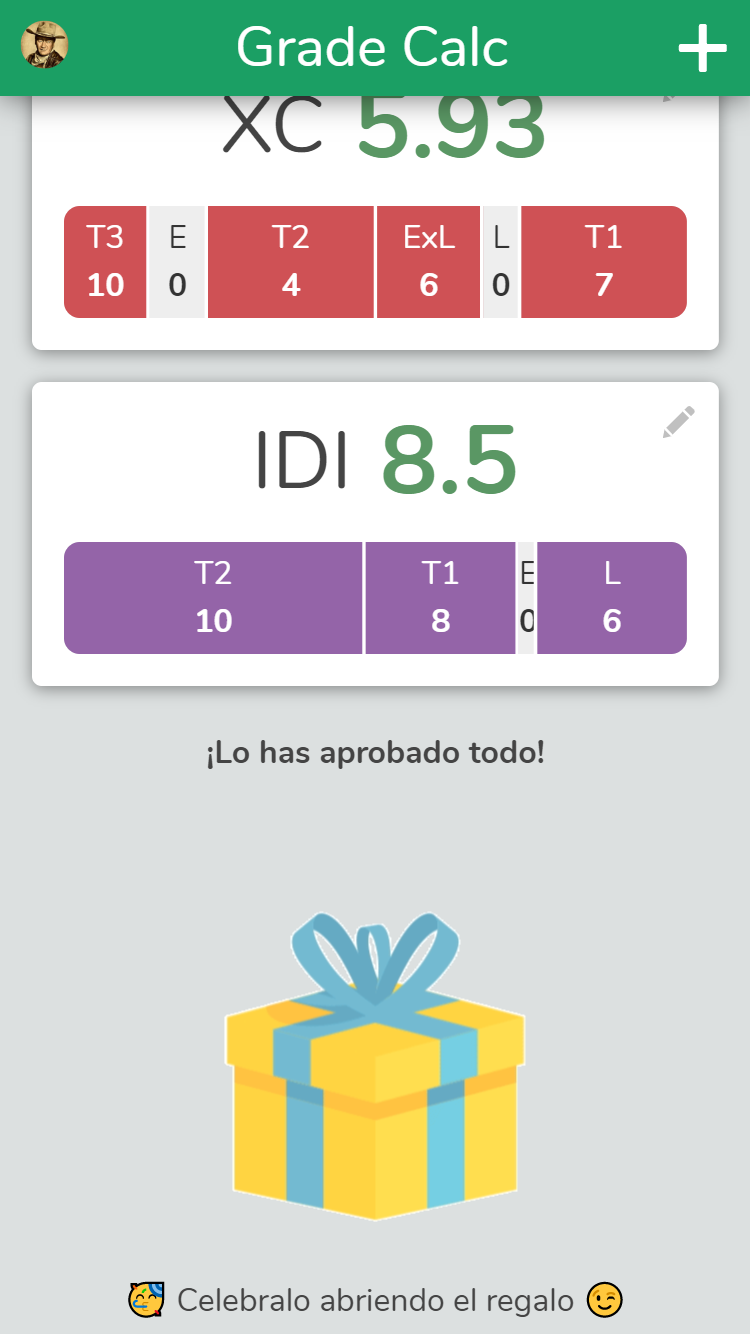
\includegraphics[width=\textwidth]{media/screenshots/screenshot-gift-1.png}
        \caption{Animation 1}
    \end{subfigure}
    \begin{subfigure}[b]{0.23\textwidth-0.1cm}
        \centering
        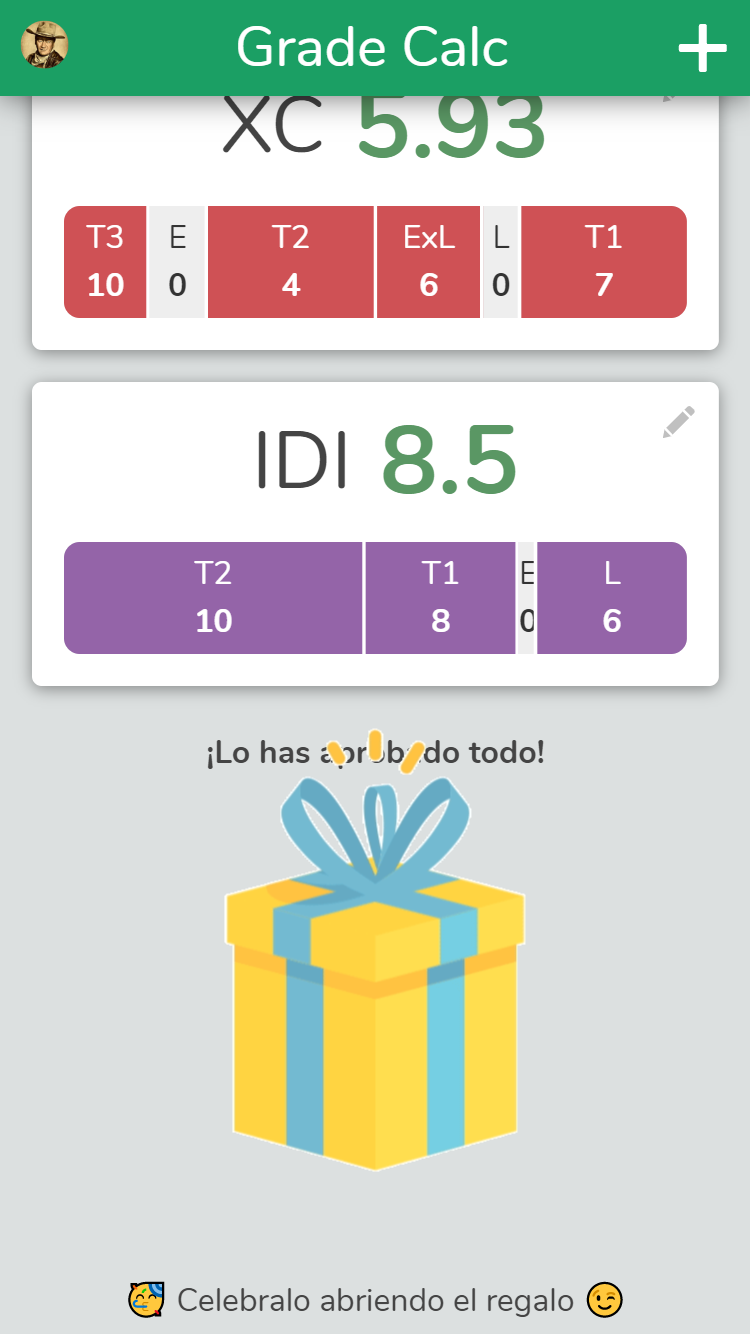
\includegraphics[width=\textwidth]{media/screenshots/screenshot-gift-2.png}
        \caption{Animation 2}
    \end{subfigure}
    \begin{subfigure}[b]{0.23\textwidth-0.1cm}
        \centering
        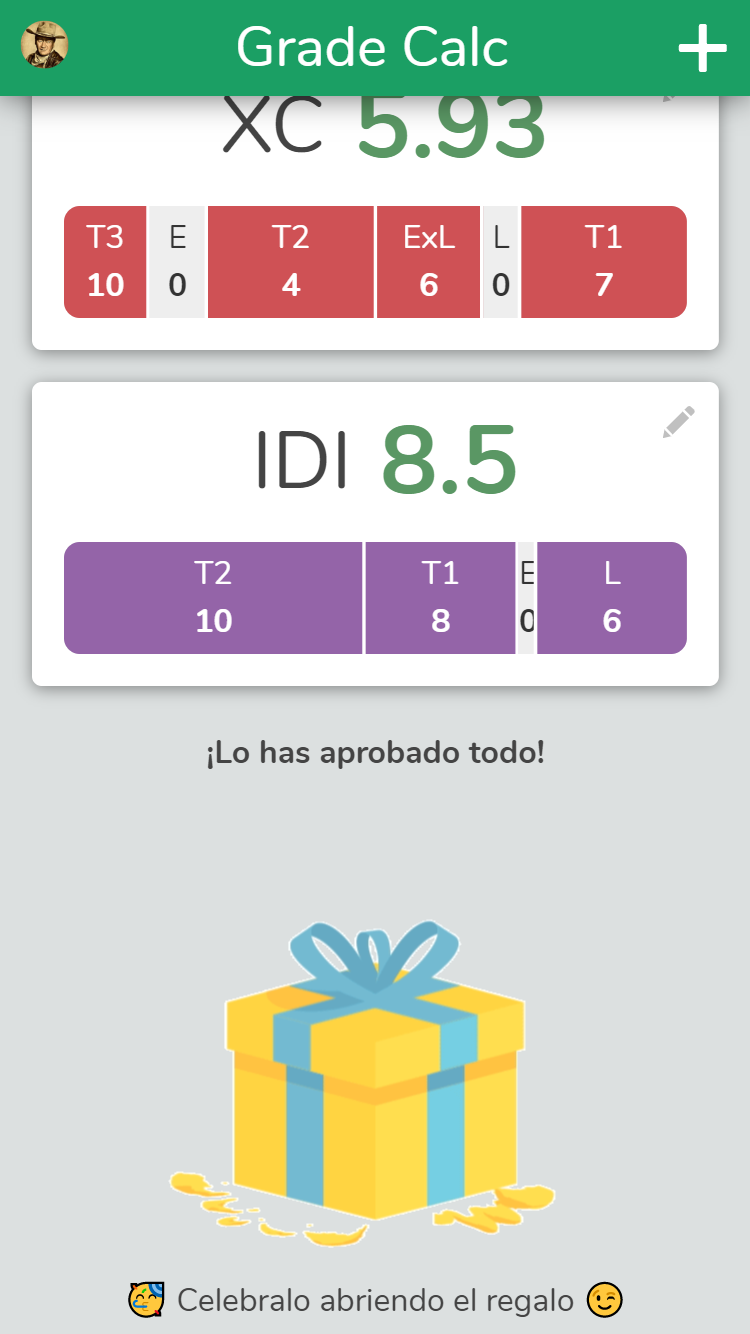
\includegraphics[width=\textwidth]{media/screenshots/screenshot-gift-3.png}
        \caption{Animation 3}
    \end{subfigure}
    \begin{subfigure}[b]{0.23\textwidth-0.1cm}
        \centering
        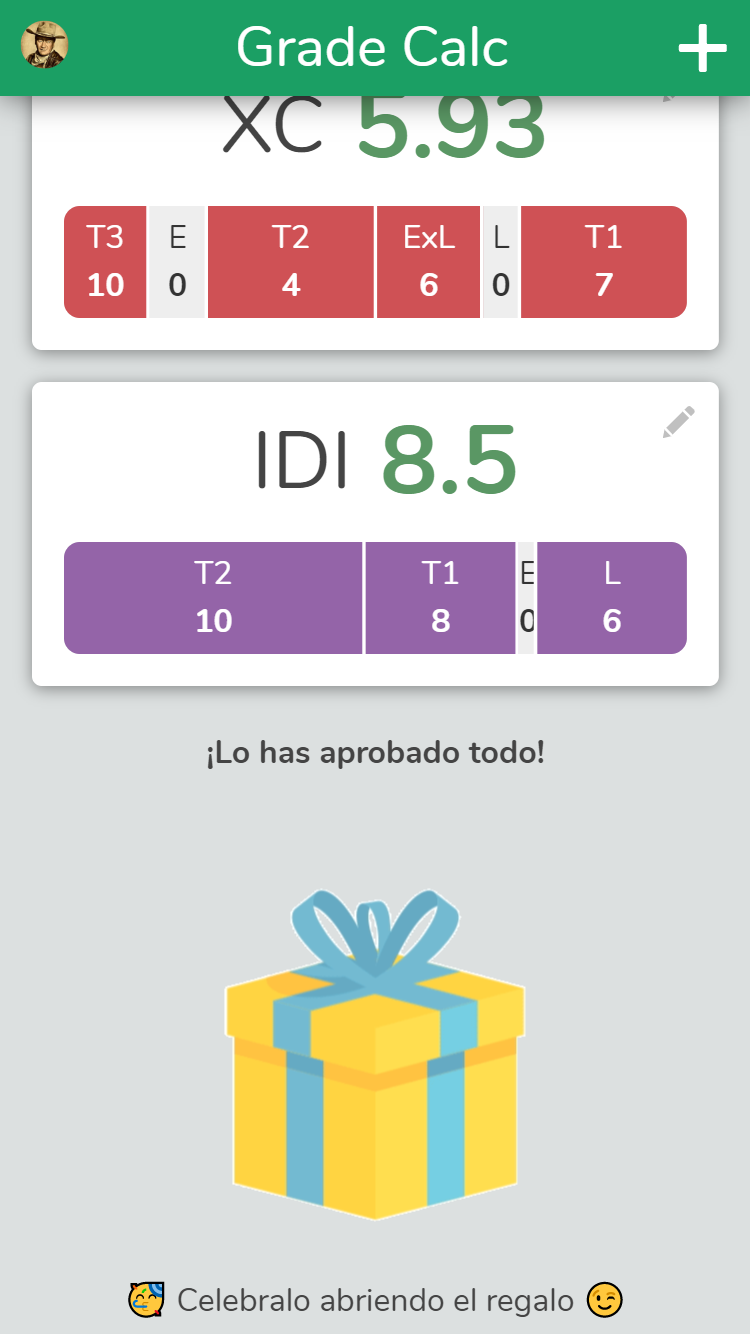
\includegraphics[width=\textwidth]{media/screenshots/screenshot-gift.png}
        \caption{Animation 4}
    \end{subfigure}
    \caption{Surprise gift animation}
    \label{fig:gift-animation}
\end{figure}
\vfill

\clearpage\newpage

When the gift is clicked, the background turns black, recalling a cinema switching off the lights, and a video appears at the bottom of the screen (Fig. \ref{fig:congratulations-video}). The video plays automatically in a loop and it's changed over time, to keep being engaging. The one right now the featured video is the famous \textit{Congratulations!!!!} meme\cite{congratulations}, it's a parody of the EVA\footnote{Neon Genesis Evangelion, an anime and manga series } ending\cite{congratulations-parody}.

Having this feature motivates students to show the app to their friends because they find it funny and interesting. It also engages users to fill their grades to unlock the gift. This is a gamification technique.

\vfill
\begin{figure}[ht!]
    \begin{subfigure}[b]{0.757\textwidth-0.1cm}
        \centering
        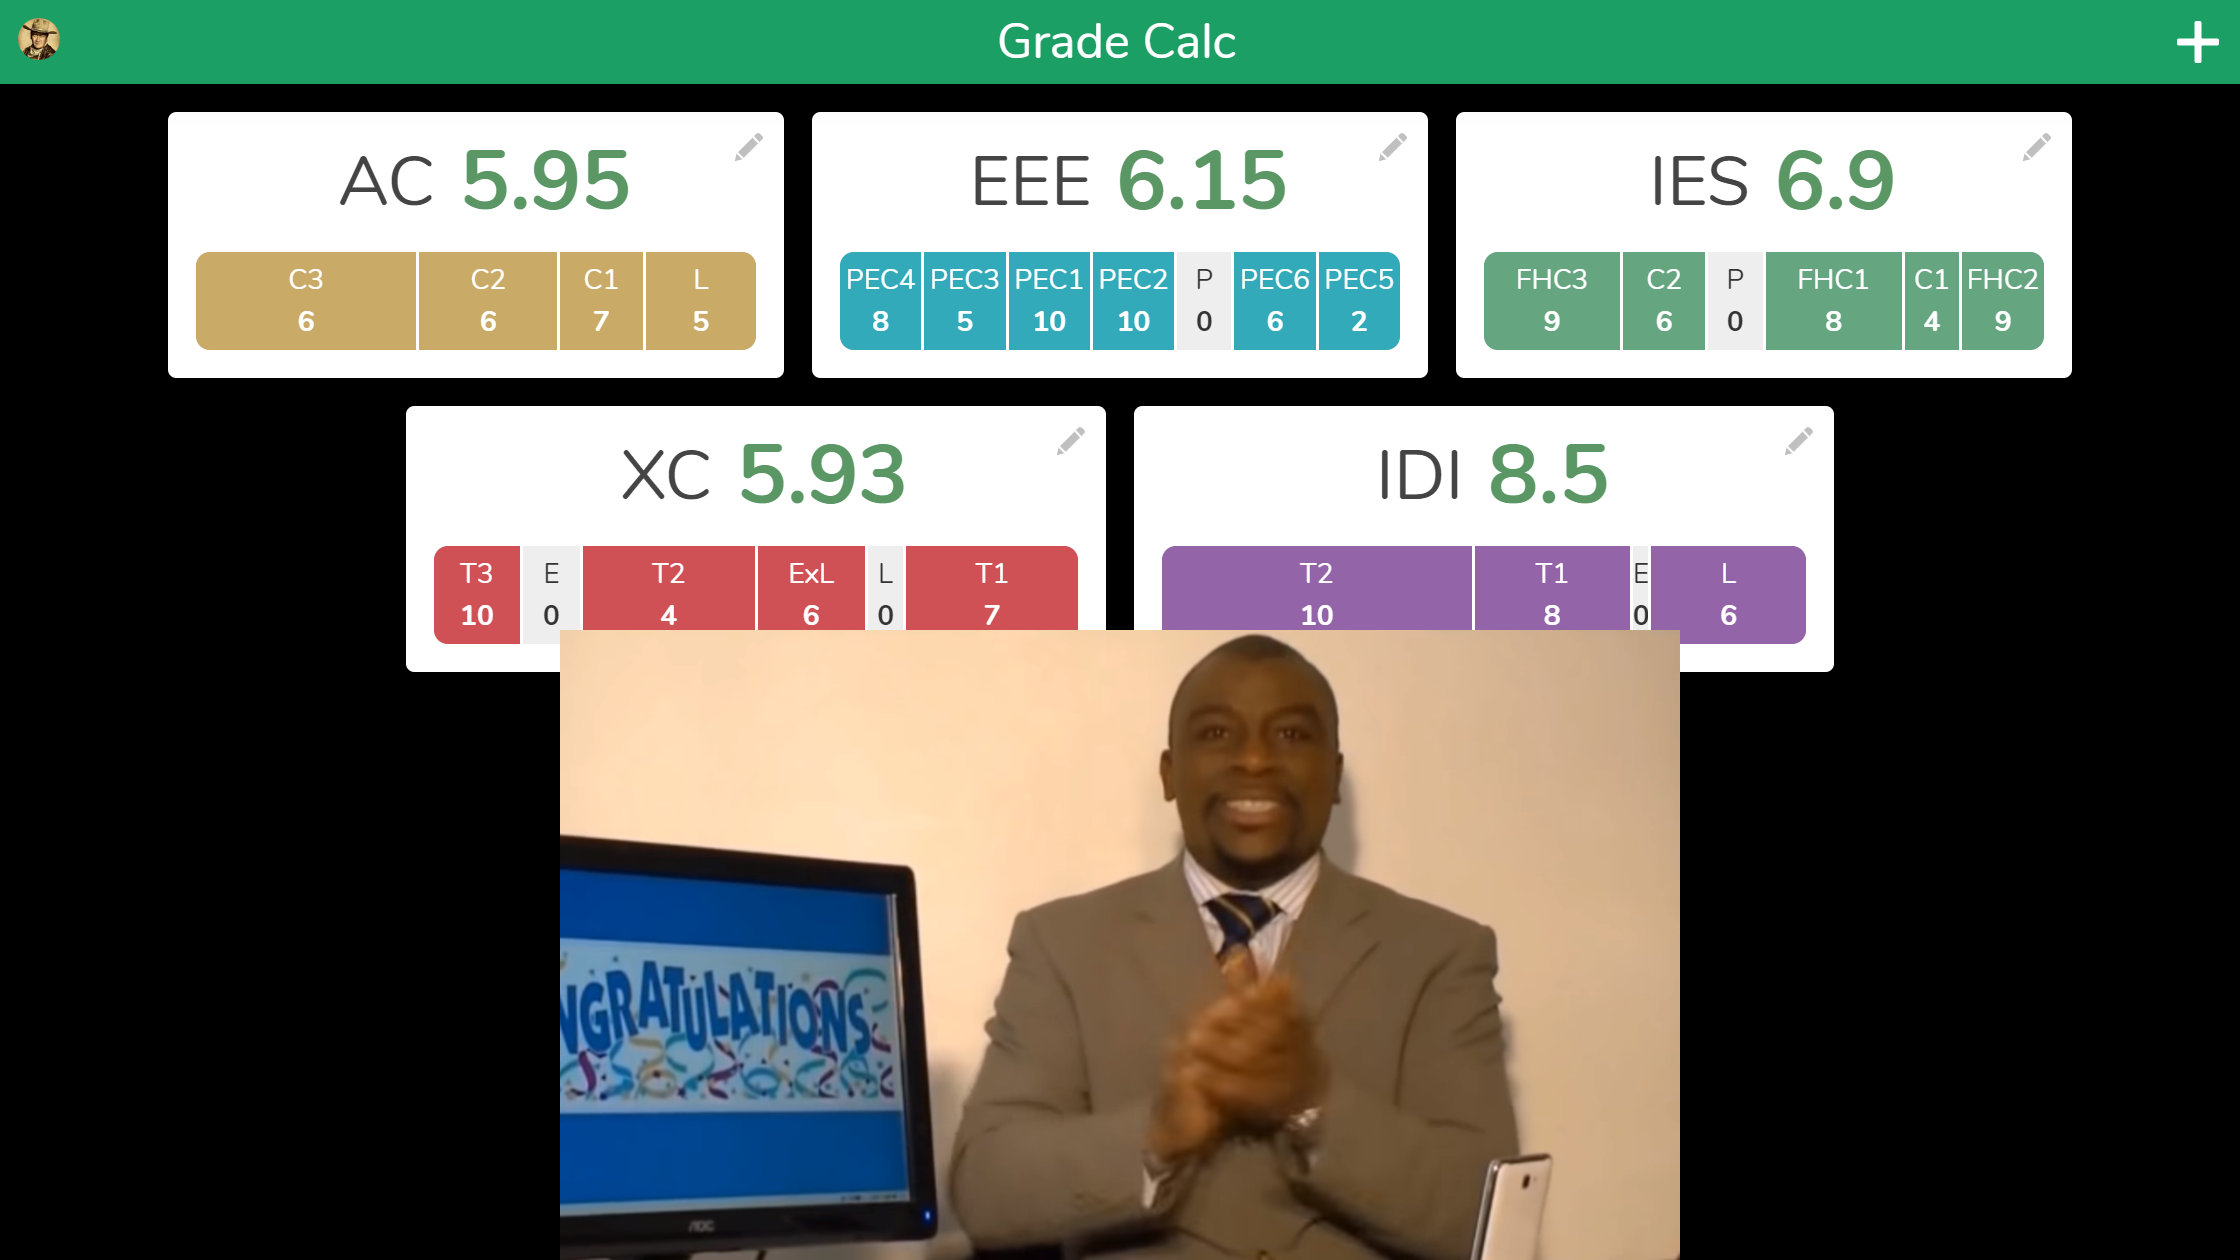
\includegraphics[width=\textwidth]{media/screenshots/screenshot-easter-egg-pc.png}
        \caption{Desktop version}
    \end{subfigure}
    \hfill
    \begin{subfigure}[b]{0.243\textwidth-0.1cm}
        \centering
        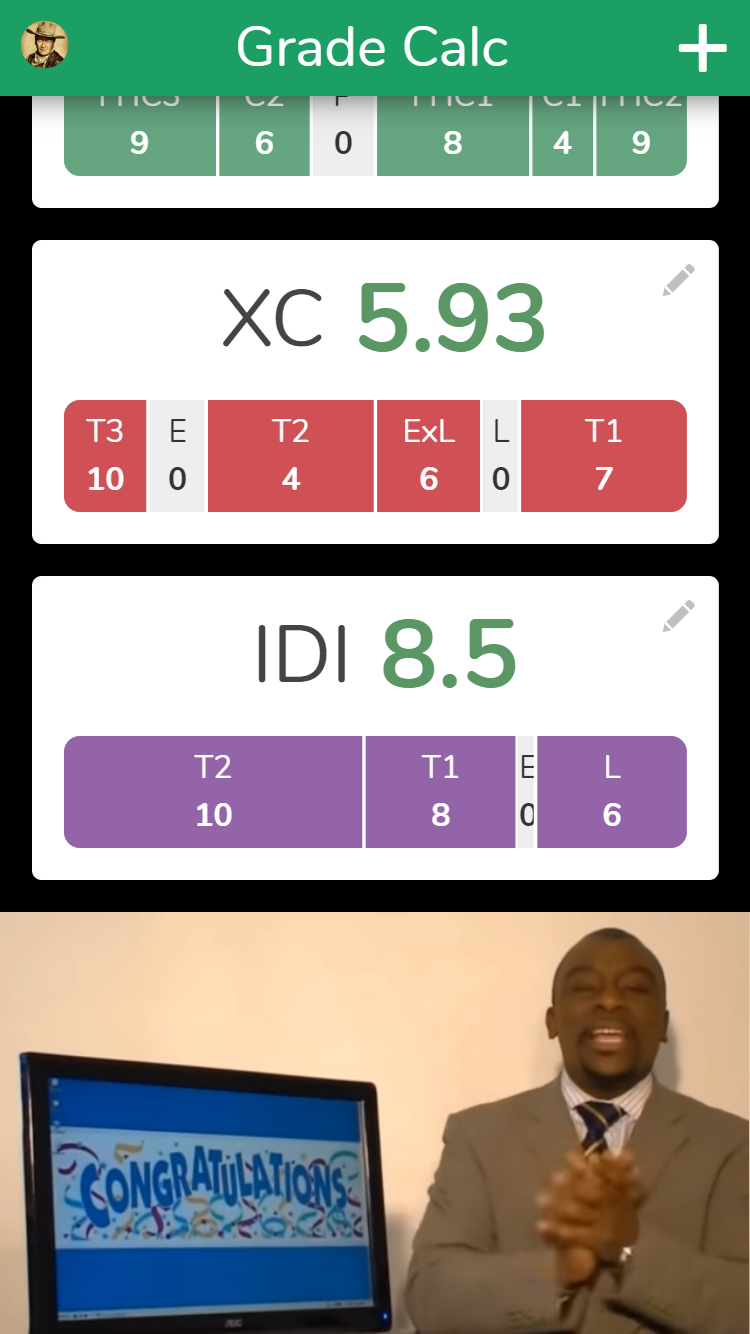
\includegraphics[width=\textwidth]{media/screenshots/screenshot-easter-egg.png}
        \caption{Mobile version}
    \end{subfigure}
    \caption{Congratulations}
    \label{fig:congratulations-video}
\end{figure}
\vfill
